% !TEX program = pdflatex
% !TEX encoding = UTF-8 Unicode

% TFG basado en la plantilla de la clase `scrbook` del paquete
% KOMA-script para la elaboración de un TFG siguiendo las
% directrices del la comisión del Grado en Matemáticas de
% la Universidad de Granada.

% Autor de la plantilla: Francisco Torralbo Torralbo
% miércoles, 29 de abril de 2020

% Autor de la memoria: Blanca Cano Camarero

\documentclass{scrbook}

\KOMAoptions{%
  fontsize=10pt,        % Tamaño de fuente
  paper=a4,             % Tamaño del papel
  headings=normal,      % Tamaño de letra para los títulos: small, normal, big
  % parskip=half,         % Espacio entre párrafos: full (una línea) o half (media línea)
  headsepline=false,    % Una linea separa la cabecera del texto
  cleardoublepage=empty,% No imprime cabecera ni pie en páginas en blanco
  chapterprefix=false,  % No antepone el texto "capítulo" antes del número
  appendixprefix=false,	% No antepone el texto "Apéndice" antes de la letra
  listof=totoc,		    	% Añade a la tabla de contenidos la lista de tablas y figuras
  index=totoc,			    % Añade a la talba de contenidos una entrada para el índice
  bibliography=totoc,	  % Añade a la tabla de contenidos una entrada para bibliografía
  BCOR=5mm,           % Reserva margen interior para la encuadernación.
                        % El valor dependerá el tipo de encuadernado y del grosor del libro.
  DIV=10,             % Cálcula el diseño de página según ciertos
                        % parámetros. Al aumentar el número aumentamos el ancho de texto y disminuimos el ancho del margen. Una opción de 14 producirá márgenes estrechos y texto ancho.
}

% INFORMACIÓN PARA LA VERSIÓN IMPRESA
% Si el documento ha de ser impreso en papel de tamaño a4 pero el tamaño del documento (elegido en \KOMAoptions con la ocpión paper) no es a4 descomentar la línea que carga el paquete `crop` más abajo. El paquete crop se encargará de centrar el documento en un a4 e imprimir unas guías de corte. El procedimiento completo para imprenta sería el siguiente:
% 0. Determinar, según el tipo de encuadernación del documento, el ancho reservado para el proceso de encuadernación (preguntar en la imprenta), es decir, la anchura del área del papel que se pierde durante el proceso de encuadernación. Fijar la varibale BCOR de \KOMAoptions a dicho valor.
% 1. Descomentar la siguiente línea e imprimir una única página con las guías de corte
% 2. Cambiar la opción `cross` por `cam` (o `off`) en el paquete crop y volver a compilar. Imprimir el documento (las guías de corte impresas no inferfieren con el texto).
% 3. Usar la página con las guías impresas en el punto 1 para cortar todas las páginas.

% \usepackage[a4, odd, center, pdflatex, cross]{crop} % Permite imprimir el documento en un a4 (si el tamaño es más pequeño) mostrando unas guías de corte. Útil para imprenta.

% VERSIÓN ELECTRÓNICA PARA TABLETA
% Las opciones siguientes seleccionan un tamaño de impresión similar a una tableta de 9 pulgadas con márgenes estrechos. Útil para producir una versión en pdf para ser leída en una tableta en lugar de impresa.
% Para que la portada quede centrada correctamente hay que editar el
% archivo `portada.tex` y eliminar el entorno `addmargin`

% \KOMAoptions{fontsize=10pt, paper=19.7104cm:14.7828cm, twoside=false, BCOR=0cm, DIV=14}

% ---------------------------------------------------------------------
%	PAQUETES
% ---------------------------------------------------------------------

% CODIFICACIÓN E IDIOMA
% ---------------------------------------------------------------------
\usepackage[utf8]{inputenc} 			    % Codificación de caracteres

% Selección del idioma: cargamos por defecto inglés y español (aunque este último es el idioma por defecto para el documento). Cuando queramos cambiar de idioma escribiremos:
% \selectlanguage{english} o \selectlanguage{spanish}

\usepackage[english, spanish, es-nodecimaldot, es-noindentfirst, es-tabla]{babel}

% Opciones cargadas para el paquete babel:
  % es-nodecimaldot: No cambia el punto decimal por una coma en modo matemático.
  % es-noindentfirst: No sangra los párrafos tras los títulos.
  % es-tabla: cambia el título del entorno `table` de "Cuadro" a "Tabla"

% Otras opciones del paquete spanish-babel:
  \unaccentedoperators % Desactiva los acentos en los operadores matemáticso (p.e. \lim, \max, ...). Eliminar esta opción si queremos que vayan acentuados

% MATEMÁTICAS
% ---------------------------------------------------------------------
\usepackage{amsmath, amsthm, amssymb} % Paquetes matemáticas
\usepackage{mathtools}                % Añade mejoras a amsmath
\mathtoolsset{showonlyrefs=true}      % sólo se numeran las ecuaciones que se usan
\usepackage[mathscr]{eucal} 					% Proporciona el comando \mathscr para
                                      % fuentes de tipo manuscrito en modo matemático sin sobreescribir el comando \mathcal

% TIPOGRAFÍA
% ---------------------------------------------------------------------
% El paquete microtype mejora la tipografía del documento.
\usepackage[activate={true,nocompatibility},final,tracking=true,kerning=true,spacing=true,factor=1100,stretch=10,shrink=10]{microtype}

% Las tipografías elegidas para el documento son las siguientes
% Normal font: 			URW Palladio typeface.
% Sans-serif font: 	Iwona
% Monospace font: 	Inconsolata
% Consultar http://www.tug.dk/FontCatalogue/ para seleccionar otra tipografía.
% Es conveniente elegir aquellas que tienen soporte matemático.
\usepackage[T1]{fontenc}
\usepackage[sc, osf]{mathpazo} \linespread{1.05}
\usepackage[scaled=.95,type1]{cabin} % sans serif in style of Gill Sans
\usepackage{inconsolata}
% \renewcommand{\sfdefault}{iwona}


% Selecciona el tipo de fuente para los títulos (capítulo, sección, subsección) del documento.
\setkomafont{disposition}{\sffamily\bfseries}

% Cambia el ancho de la cita. Al inicio de un capítulo podemos usar el comando \dictum[autor]{cita} para añadir una cita famosa de un autor.
\renewcommand{\dictumwidth}{0.45\textwidth}

\recalctypearea % Necesario tras definir la tipografía a usar.

% TABLAS, GRÁFICOS Y LISTADOS DE CÓDIGO
% ---------------------------------------------------------------------
\usepackage{booktabs}
% \renewcommand{\arraystretch}{1.5} % Aumenta el espacio vertical entre las filas de un entorno tabular

\usepackage{xcolor, graphicx}
% Carpeta donde buscar los archivos de imagen por defecto
\graphicspath{{img/}}

% IMAGEN DE LA PORTADA
% Existen varias opciones para la imagen de fondo de la portada del TFG. Todas ellas tienen en logotipo de la universidad de Granada en la cabecera. Las opciones son las siguientes:
% 1. portada-ugr y portada-ugr-color: diseño con marca de agua basada en el logo de la UGR (en escala de grises y color).
% 2. portada-ugr-sencilla y portada-ugr-sencilla-color: portada únicamente con el logotipo de la UGR en la cabecera.
\usepackage{eso-pic}
\newcommand\BackgroundPic{%
	\put(0,0){%
		\parbox[b][\paperheight]{\paperwidth}{%
			\vfill
			\centering
      % Indicar la imagen de fondo en el siguiente comando
			
\includegraphics[width=\paperwidth,height=\paperheight,%
			keepaspectratio]{portada/portada-ugr-sencilla-color}%
			\vfill
}}}

\usepackage{listings} % Para la inclusión de trozos de código

% CABECERAS
% ---------------------------------------------------------------------
% Si queremos modificar las cabeceras del documento podemos usar el paquete
% `scrlayer-scrpage` de KOMA-Script. Consultar la documentación al respecto.
% \usepackage[automark]{scrlayer-scrpage}

% VARIOS
% ---------------------------------------------------------------------

%\usepackage{showkeys}	% Muestra las etiquetas del documento. Útil para revisar las referencias cruzadas.

% ÍNDICE
% Para generar el índice hay que compilar el documento con MakeIndex. Generalmente los editores se encargan de ello automáticamente.
% ----------------------------------------------------------------------
% \index{} para añadir un elemento
% \index{main!sub} para añadir un elementos "sub" bajo la categoría "main".
% \index{termino|textbf} para dar formato al número de página (negrita).
% \index{termino|see{termino relacionado}} para crear una referencia cruzada

% Ejemplo: \index{espacio homogéneo}, \index{superficie!mínima}, \index{esfera|see{espacio homogéneo}}
\usepackage{makeidx}
%\usepackage{showidx} % Muestra en el margen del documento las entradas añadidas al índice. Útil para revisar el documento. Si está activo el índice no se genera
\makeindex

% ---------------------------------------------------------------------
% COMANDOS Y ENTORNOS
% ---------------------------------------------------------------------
% Cargamos un archivo externo donde hemos incluido todos los comandos
% propios que vamos a usar en el documento.
% DEFINICIÓN DE COMANDOS Y ENTORNOS

% CONJUNTOS DE NÚMEROS

  \newcommand{\N}{\mathbb{N}}     % Naturales
  \newcommand{\R}{\mathbb{R}}     % Reales
  \newcommand{\Z}{\mathbb{Z}}     % Enteros
  \newcommand{\Q}{\mathbb{Q}}     % Racionales
  \newcommand{\C}{\mathbb{C}}     % Complejos

% Otros espacios 
\newcommand{\D}{\mathcal{D}} % Conjunto de datos de entrenamiento

  %%%%%%%%% Mis comandos %%%%%%%%%
% Para escribir código y pseudo código  
\usepackage{minted}
\usemintedstyle{friendly}
\definecolor{sutilGreen}{rgb}{0.850, 0.996, 0.807} % para el fondo del código
\definecolor{sutilBackground}{rgb}{0.933, 0.905, 0.866}
\newminted{code}{
  frame=single,
  framesep=10pt,
  baselinestretch=1.2,
  bgcolor=sutilBackground, 
  %linenos 
}
\newminted{example}{frame=single,
  framesep=10pt,
  baselinestretch=1.2,
  %bgcolor=sutilBackground, 
  %linenos
}
\usepackage{algorithmic}
% Para la definición de redes neuronales de una sola capa 
\newcommand{\Hu}{\mathcal{H}(X,Y)}  % Espacio de las redes neuronales

% Notas en el margen
\usepackage{sidenotes}
  \newcommand{\afines}{\mathcal{A}(\R^d)}
  \newcommand{\pmc}{\mathcal{H}_G(\R^d,\R)}%{\sum ^r (G)}  % Red neurona una capa una salida
  \newcommand{\pmcg}{ \sum \prod^d (G)} % Generalización red neuronal
  \newcommand{\fC}{\mathcal{C}(\R^d)} %conjunto de funciones continuas en R^r -> R
  \newcommand{\fM}{\mathcal{M}(\R^d)} % Conjunto funiones medibles
  \newcommand{\rrnn}{ \mathcal{H}(\R^d,\R)} % Red neuronal  sin subíndice
  \newcommand{\rrnng}{ \sum \prod^d (\psi)} % Red neuronal  generalizado
  \newcommand{\dist}{\rho_{\mu}}     % Distancia de una medida
  \newcommand{\dlp}{\rho_{p}} % Distancia de los espacios Lp
  % Múltiples salidas 
  \newcommand{\fCC}{\mathcal{C}(\R^d ,\R^s)}
  \newcommand{\fMM}{\mathcal{M}(\R^d , \R^s)}
  \newcommand{\rrnnmc}{ \mathcal{H}(\R^d,\R^s)} 
  \newcommand{\rrnnsmn}{ \mathcal{H}_n(\R^d,\R^s)} % Red neuronal salida múltiple con n neuronas
  \newcommand{\rrnngmc}{ \sum \prod^{d,s} (\psi)} 
  %%%%%%%%% Mis comandos %%%%%%%%%5
\usepackage{sidenotes} % Notas en el margen
\newcommand{\margenimagen}{
  \newgeometry{
      left=2.5cm, % Margen izquierdo
    right=5cm, % Margen derecho
    bottom=2.5cm % Margen inferior}
  }
}
\usepackage{caption}
\usepackage{subcaption}

% TEOREMAS Y ENTORNOS ASOCIADOS

  % \newtheorem{theore<m}{Theorem}[chapter]
  \newtheorem*{teorema*}{Teorema}
  \newtheorem{teorema}{Teorema}[chapter]
  \newtheorem{proposicion}{Proposición}[chapter]
  \newtheorem{lema}{Lema}[chapter]
  \newtheorem{corolario}{Corolario}[chapter]

    \theoremstyle{definition}
  \newtheorem{definicion}{Definición}[chapter]
  \newtheorem{ejemplo}{Ejemplo}[chapter]

    \theoremstyle{remark}
  \newtheorem{observacion}{Observación}[chapter]


\DeclareMathOperator{\sign}{signo}
\usepackage[inline]{enumitem}
\usepackage{mathtools}
\usepackage[spanish,onelanguage,linesnumbered,ruled,vlined]{algorithm2e}
\usepackage{listingsutf8}
\lstset{language=Python,
        literate=
          {ó}{{\'o}}1
          {í}{{\'i}}1
          {á}{{\'a}}1
          {ú}{{\'u}}1
          {é}{{\'e}}1
          {ñ}{{\v{n}}}1
}
\usepackage{tocloft}
\setlength{\cftfignumwidth}{2.55em}
\DeclareMathOperator*{\argmin}{arg\,min}

\SetKwRepeat{Struct}{struct \{}{\}}%

% Para las notas del margen 
%Nota los colores seleccionados han sido creados con una paleta inclusiva
% https://palett.es/6a94a8-013e3b-7eb645-31d331-26f27d
\definecolor{darkRed}{rgb}{0.2,1,0.7}%{ 0.149, 0.99, 0.49}%{1,0.1,0.1}
\definecolor{dark_green}{rgb}{0, 0.24, 0.23} %{0.2, 0.7, 0.2}
\definecolor{blue}{rgb}{0.61, 0.98, 0.759} % sobreeescribimos el azul
\newcommand{\smallMarginSize}{1.8cm}
\newcommand{\bigMarginSize}{3cm}
\newcommand{\maginLetterSize}{\scriptsize}%{\footnotesize} %{\scriptsize}%

% Para los iconos 
\usepackage{fontawesome}
% Alias aclaraciones 
% dark_green
\newcommand{\iconoAclaraciones}{\faQuestionCircleO $\quad$} %\faQuestionCircleO
% blue
\newcommand{\iconoProfundizar}{\faSearch  $\quad$}
\newcommand{\iconoClave}{\faLightbulbO  $\quad$} % \faLightbulbO %\faKey

% Contenido original 
\usepackage{lipsum}
\usepackage[%
linewidth=5pt,
outerlinecolor=red,
outerlinewidth=5pt,
innerlinewidth=1pt,
outerlinecolor=red,
roundcorner=5pt
%middlelinecolor= yellow,
middlelinewidth=0.4pt,
%roundcorner=1pt,
topline = false,
rightline = false,
leftline = false,
bottomline = false,
rightmargin=0pt,
skipabove=7pt,
skipbelow=7pt,
leftmargin=-1cm,
backgroundcolor=black!7,
%innerleftmargin=1cm,
%innerrightmargin=0pt,
%innertopmargin=0pt,
%innerbottommargin=0pt,
frametitlebackgroundcolor=yellow!100,
]{mdframed}
 
\newenvironment{aportacionOriginal}
  {\mdfsetup{
    frametitle=\textcolor{white}{\Large Aportación original}
    %frametitle={\colorbox{black!7}{ \textcolor{white}{\Large Aportación original}}},
    %frametitleaboveskip=-\ht\strutbox,
    %frametitlealignment=\center
    }
  \begin{mdframed}%
  }
  {\end{mdframed}}

  % ancho imágenes en tabla
  \newcommand{\coeficienteAncho}{.3}

% Paquetes para citas
\usepackage{csquotes}
\let\oldenquote\enquote
\renewcommand{\enquote}[1]{{\itshape\oldenquote{#1}}}
\usepackage{epigraph} %este es para las que salen a la derecha




% --------------------------------------------------------------------
% INFORMACIÓN DEL TFG Y EL AUTOR
% --------------------------------------------------------------------
\usepackage{xspace} % Para problemas de espaciado al definir comandos

\newcommand{\miTitulo}{Optimización de redes neuronales\xspace}
\newcommand{\miNombre}{Blanca Cano Camarero\xspace}
\newcommand{\miGrado}{Doble Grado en Ingeniería Informática y Matemáticas}
\newcommand{\miFacultad}{Escuela Técnica Superior de Ingenierías Informática y de Telecomunicación \\ Facultad de Ciencias}
\newcommand{\miUniversidad}{Universidad de Granada}
% Añadir tantos tutores como sea necesario separando cada uno de ellos
% mediante el comando `\\\medskip` y una línea en blanco
\newcommand{\miTutor}{
  Juan Julián Merelo Guervós\\ \emph{Arquitectura y tecnología de computadores}
  \\\medskip

  Francisco Javier Meri de la Maza\\ \emph{Análisis matemático}
}
\newcommand{\miCurso}{2021-2022\xspace}

% HYPERREFERENCES
% --------------------------------------------------------------------
\usepackage{xurl}
\usepackage[pagebackref]{hyperref}
% Opciones para el paquete hyperref
%----------------------------------

\hypersetup{%
  % hidelinks,            % Enlaces sin color ni borde. El borde no se imprime
  linkbordercolor=0.8 0 0,
  citebordercolor=0 0.8 0,
  citebordercolor=0 0.8 0,
  colorlinks = true,            % Color en texto de los enlaces. Comentar esta línea o cambiar `true` por `false` para imprimir el documento.
  linkcolor = [rgb]{0.5, 0, 0}, % Color de los enlaces internos
  urlcolor = [rgb]{0, 0, 0.5},  % Color de los hipervínculos
  citecolor = [rgb]{0, 0.5, 0}, % Color de las referencias bibliográficas
	pdftitle={\miTitulo},%
	pdfauthor={\textcopyright\ \miNombre, \miFacultad, \miUniversidad},%
  pdfsubject={Trabajo de fin de Grado},%
	pdfkeywords={},%
	pdfcreator={pdfLaTeX},%
}

% Redefinición del estilo para mostrar las referencias cruzadas en la bibliografía.
\renewcommand*{\backref}[1]{}
\renewcommand*{\backrefalt}[4]{{\footnotesize [%
    \ifcase #1 No citado%
    \or Citado en pág.~#2%
    \else Citado en págs. #2%
    \fi%
]}}

% Etiquetas en español para el comando \autoref
\def\chapterautorefname{Capítulo}
\def\appendixautorefname{Apéndice}
\def\sectionautorefname{Sección}
\def\subsectionautorefname{Subsección}
\def\figureautorefname{Fig.}
\def\tableautorefname{Tabla}

\def\teoremaautorefname{Teorema}
\def\proposicionautorefname{Proposición}
\def\lemaautorefname{Lema}
\def\corolarioautorefname{Corolario}
\def\definicionautorefname{Def.}
\def\observacionautorefname{Observación}
\def\ejemploautorefname{E.j.}

% Pone automáticamente un parántesis para las ecuaciones
\def\equationautorefname~#1\null{Ec.~(#1)\null}

% Extra
\def\algorithmautorefname{Algoritmo}


\begin{document}

% --------------------------------------------------------------------
% FRONTMATTER
% -------------------------------------------------------------------
%\frontmatter % Desactiva la numeración de capítulos y usa numeración romana para las páginas

% \pagestyle{plain} % No imprime cabeceras

% !TeX root = ../libro.tex
% !TeX encoding = utf8

%*******************************************************
% Titlepage
%*******************************************************
\begin{titlepage}
  \AddToShipoutPicture*{\BackgroundPic}
  \phantomsection
  \pdfbookmark[1]{Título}{title}

  % Para que el título esté centrado en la página.
  % Los valores numéricos deberán elegirse de acuerdo con el diseño de
  % página (sobre todo si se cambia la opción BCOR o DIV).
  \begin{addmargin}[2.575cm]{0cm}
  \begin{flushleft}
    \Large
    \hfill\vfil

    \large{\textsf{\miFacultad}}
    \vfill

    {\large\textsc\miGrado} \vfill


    {\large\textsc{trabajo de fin de grado}}

    \vspace*{0.5cm}

    \begingroup
    \centering
    \Huge{\miTitulo}
    \endgroup

    \vfill\vfill\vfill\vfill

    \textsf{\normalsize{Presentado por:}}\\
    {\normalsize\textrm{\miNombre}}
    \bigskip

    \textsf{\normalsize{Tutores:}}\\
    {\normalsize\rmfamily \miTutor}

    \bigskip
    \textsf{\normalsize{Curso académico \miCurso}}
  \end{flushleft}
  \end{addmargin}

\end{titlepage}
\cleardoublepage
\endinput

% !TeX root = ../libro.tex
% !TeX encoding = utf8

%*******************************************************
% Little Dirty Titlepage
%*******************************************************

\thispagestyle{empty}

\begin{center}
  \large

  \vspace*{\stretch{1}}

  \begingroup
  \huge{\miTitulo} \\ \bigskip
  \endgroup

  \textrm{\miNombre}

  \vspace{\stretch{5}}

\end{center}

\newpage
\thispagestyle{empty}

\hfill

\vfill

\noindent\miNombre \textit{\miTitulo}.

\noindent Trabajo de fin de Grado. Curso académico \miCurso.
\\
\\
\begin{minipage}[t]{0.25\textwidth}
  \flushleft
  \textbf{Responsables de tutorización}
\end{minipage}
\begin{minipage}[t]{0.45\textwidth}
  \flushleft
  \miTutor
\end{minipage}
\begin{minipage}[t]{0.30\textwidth}
  \flushright
  \miGrado
  \medskip

  \miFacultad
  \medskip

  \miUniversidad
\end{minipage}
\begin{flushleft}
\end{flushleft}

\endinput

%% !TeX root = ../libro.tex
% !TeX encoding = utf8
%
%*******************************************************
% Declaración de originalidad
%*******************************************************

\thispagestyle{empty}

\hfill\vfill

\textsc{Declaración de originalidad}\\\bigskip

Dña. \miNombre \\\medskip

Declaro explícitamente que el trabajo presentado como Trabajo de Fin de Grado (TFG), correspondiente al curso académico \miCurso, es original, entendida esta, en el sentido de que no ha utilizado para la elaboración del trabajo fuentes sin citarlas debidamente.
\medskip

En Granada a \today
\begin{flushleft}
Fdo: \miNombre

\end{flushleft}

\vfill

\endinput

% !TeX root = ../libro.tex
% !TeX encoding = utf8
%
%*******************************************************
% Resumen
%*******************************************************

% \manualmark
% \markboth{\textsc{Introducción}}{\textsc{Introducción}}

\chapter*{Resumen}\label{ch:resumen}
%\addcontentsline{toc}{chapter}{Resumen}

Existe en la actualidad un desequilibrio entre resultados empíricos 
y teóricos de redes neuronales llegando incluso a contradicción
 (como se comenta en la introducción del capítulo 
 \ref{chapter:Introduction-neuronal-networks}), será por tanto
nuestro primer objetivo construir una teoría sólida
que de cabida a 
 optimizaciones de fundamento teórico; 
una revisión y
 purga de cualquier artificio existente sobre 
 redes neuronales carente de fundamento matemático. 

Como resultado de ello se ha creado e implementado 
un nuevo modelo de red neuronal así como sus 
métodos de aprendizaje y evaluación. 
Además se ha propuesto un criterio de selección de 
funciones de activación y un algoritmo de 
inicialización de pesos que mejora los ya existentes. Todos los resultados han conducido a la creación de 
la biblioteca \textit{OptimizedNeuralNetwork.jl}, que contiene la implementación de nuestros modelos y métodos optimizados. 


La estructura de la memoria es la siguiente: 

\begin{itemize}
    \item \textbf{Capítulo \ref{ch00:methodology}: Descripción de la metodología seguida.} Se ha organizado el proyecto de acorde a una filosofía de desarrollo ágil, basada en la metodología de personas, historias de usuario, hitos y test. Tal método ha conducido e hilado desde el comienzo tanto el desarrollo teórico como el técnico a la par que  salvaguardaba la corrección de cada paso. 
    \item \textbf{Capítulo \ref{chapter:Introduction-neuronal-networks}: Descripción del problema de aprendizaje.} Se introduce las características y tipo de problemas del aprendizaje automático. Además se clarifica cuáles tratan de resolver las redes neuronales. 
    \item \textbf{Capítulo \ref{ch03:teoria-aproximar}: Teoría de la aproximación.} Se muestran los problemas y virtudes que presenta un enfoque clásico  de teoría de la aproximación frente a problemas de aprendizaje. En pos de solventar tales impedimentos,  
    se sitúa esta teoría como el germen de 
    las redes neuronales.
    Concretamente se desarrolla la teoría necesaria hasta demostrar el teorema de \textit{Stone-Weierstrass} y se explicarán las trabas que presentan este tipo de aproximaciones. 
    \item \textbf{Capítulo \ref{chapter4:redes-neuronales-aproximador-universal}: Introducción de las redes neuronales como aproximadores universales.} Se presenta nuestra propuesta de modelo de red neuronal y se compara con los modelos actuales. Se demuestra que nuestra definición actúa como un aproximador universal a cualquier función medible basándonos en el artículo 
    \textit{Multilayer Feedforward Networks are Universal Approximators} (\cite{HORNIK1989359}). Además se demuestran unas serie de resultados sobre cómo es la convergencia en problema de regresión y clasificación. Finalemnte se plantea si en la práctica las redes neuronales 
    verdaderamente son aproximadores universales.
    \item \textbf{Capítulo \ref{chapter:construir-redes-neuronales}: Diseño y construcción de las redes neuronales.} Se describe la implementación de las redes neuronales; esto nos permitirá una comparación  
    más profunda de nuestro modelo frente a los usuales y que nos servirá como justificación del modelo obtenido. Producto de ello son dos resultados originales sobre el sesgo y dominio de la imagen. 
    Una vez determinado el modelo concreto se
    han diseñado un algoritmo de aprendizaje, basado en \textit{Backpropagation} y otro de evaluación de redes neuronales. Además se han comparado los resultados de nuestro modelado con los utilizado usualmente. 
    \item \textbf{Capítulo \ref{funciones-activacion-democraticas-mas-demoscraticas}: Democratización de las funciones de activación.} Se pretende en este capítulo determinar qué funciones de activación son más convenientes que otras, es decir, con cuál se podría tener un menor coste computacional. 
    Para esto, no se ha tenido sólo en cuenta el coste computacional de evaluar cada función; puesto que la imagen de una función de activación repercute 
    en el número de neuronas necesarias para estar por debajo de cierto error, se ha establecido una serie de teoremas propio que determina qué funciones de activación tendrán los mismos resultados.  Gracias a tales resultados se han 
    podido agrupar a las funciones de activación y 
    para cada clase se ha tratado de determinar por medio del test de hipótesis de Wilcoxon cuál es la más rápida, resultando con esto que sin perder precisión se ha reducido el costo y tiempo en evaluación y entrenamiento de las redes neuronal. 
    
    \item \textbf{Capítulo \ref{section:inicializar_pesos}: Algoritmo de inicialización de pesos.} Se propone un algoritmo original de inicialización de los pesos de una red neuronal a 
    partir de un subconjunto de datos de la muestra. Al ser la solución de partida mejor, con este método se pretende reducir el tiempo y coste de aprendizaje de técnicas iterativas, tales como \textit{Backpropagation}.  
    
    En este capítulo se muestran además los 
    requisitos técnicos de la implementación de la biblioteca \textit{OptimizedNeuralNetwork.jl}, 
    ya que para medir la bondad del algoritmo es 
    necesario implementar todas las funcionalidades al completo. Además se han añadido en estas 
    secciones ejemplo de uso de la biblioteca. 
    \item \textbf{Capítulo \ref{ch08:genetic-selection}: Selección genética de las funciones de activación.} El uso de distintas funciones de activación presenta un 
    potencial en cuanto a reducir el error fijado un cierto número de neuronas, sin embargo esto 
    aumenta el espacio de búsqueda y por tanto la complejidad. Es aquí donde nuestro modelo 
    propuesto de red neuronal palía la situación, 
    ya que frente a los modelos convencionales, el nuestro es invariante a la posición de las 
    funciones de activación de las neuronas, lo cual
     reduce el espacio de búsqueda.  
\end{itemize}

\paragraph{PALABRAS CLAVE:}
\begin{itemize*}[label=,itemsep=1em,itemjoin=\hspace{1em}]
  \item redes neuronales
  \item optimización 
  \item funciones de activación 
  \item inicialización de pesos
\end{itemize*}

\endinput

% !TeX root = ../libro.tex
% !TeX encoding = utf8
%
%*******************************************************
% Summary
%*******************************************************

\selectlanguage{english}
\chapter*{Summary}\label{ch:summary}
%\addcontentsline{toc}{chapter}{Summar}

Nowadays experimental research in Neural Networks is more advanced than theoretical
results. 
From this we aim to establish a solid mathematical theory so as to optimize the current neural network models. 


As a result of our study, we have proposed a novel neural 
network model, and adapted and optimized
evaluation and learning methods to it. 
Moreover, we have discovered some theorems that prove the 
equivalence among some activation functions, and hence propose a new
 algorithm to initialize weights of neural networks. Thanks to the
first result, we obtain a criteria to choose the most 
suitable activation function to maintain accuracy and reduce computational costs.
 Thanks to the second one, we might accelerate 
learning convergence methods.

In addition, the models, methods and algorithms have been 
implemented in Julia, resulting in the \textit{OptimizedNeuralNetwork.jl} library. 

All the theory development, designs, decisions and results are 
written in this memory, which have the following structure: 
\begin{itemize}
 \item \textbf{Chapter \ref{ch00:methodology}: Description of the methodology followed.} We have organized our project according to an agile philosophy  based on personas methodology, user stories, milestones and tests. This method has conducted and linked mathematical and technical results and implementations, giving them coherence and validation methods. 

 \item \textbf{Chapter \ref{chapter:Introduction-neuronal-networks}: Description of the learning problem.} We defined the characteristic and type of machine learning problems. We will focus on supervised learning ones. 

 \item \textbf{Chapter \ref{ch03:teoria-aproximar}:  Approximation theory.} In order to establish a solid theory, we will start our work trying to solve machine learning problems by traditional approximation methods.  The main result we prove is the Stone Weierstrass's theorem. As a conclusion of this chapter we will achieve knowledge of the virtues and faults of traditional methods and understanding the necessity of new methods and structures such as neural networks. 

 \item \textbf{Chapter \ref{chapter4:redes-neuronales-aproximador-universal}: Neural networks are universal approximators.}  In this chapter we introduce our neural 
 network model and compare it with the conventional ones. In order to show it is well 
 defined, we will prove the universal convergence of our model to any measurable 
 function. In addition, we will give some results about how our model solves 
 classification and regression problems as its number of neurons rises. Finally, we 
 will argue if all of those math results can actually solve real life problems. The 
 idea behind the debate is the computability representation of real numbers. 

 \item \textbf{Chapter  \ref{chapter:construir-redes-neuronales}: The design and implementation of neural networks.} We will carefully  describe the design and 
 implementation of our model of neural network. Thanks to that we will obtain some 
 mathematical results about bias and classification function. This will be useful to 
 compare our model with the conventional ones and justify 
our selection. Moreover, we will explain, justify and design  learning and evaluation 
methods to our model. These methods are optimized versions of Forward Propagation and 
Backpropagation. 

\item \textbf{Chapter \ref{funciones-activacion-democraticas-mas-demoscraticas}: Democratization of activation functions.} 
We will explain in this chapter if there are better activation functions. In this 
direction we will prove two original results which show that there are families of 
activation functions that with the same conditions will solve problems with the same 
accuracy. As a result, if we compare the computational cost of the members of those 
families and choose the faster one, we will obtain a method to optimize evaluation and 
learning of neural networks without loss of accuracy. We have used the Wilcoxon 
signed-rank test as a statistical hypothesis test so as to give a rigorous study of 
our criteria. 

\item \textbf{Chapter \ref{section:inicializar_pesos}: Weight initializing algorithm.} 
Since the Backpropagation and other iterative  methods are sensitive to the initial 
value of a neural network, we will show an original method to initialize its weights 
from training data. This process not only will produce a better initial step but also 
has lower computational cost than Backpropagation.  To test the potential of this 
method we will use the Wilcoxon signed-rank test again and also, from the experiment's 
requirements we will design and create our OptimizedNeuralNetwork.jl library. In this chapter we 
will also explain every decision done during the design and implementation of the 
library in order to be as efficient as possible.	

\item \textbf{Chapter \ref{ch08:genetic-selection}: Use of genetic algorithm in the selection of activation function.} 
In this chapter we will explain a future work. Given a fixed number of neurons, the 
selection of its activation function may be crucial to reduce the train and test 
error.  However, adding more free params to the search space increases its complexity 
and at same time the cost of finding a solution.  Nevertheless, the result obtained at 
chapter \ref{funciones-activacion-democraticas-mas-demoscraticas} and a property of our neural model will reduce the space complexity.

\item \textbf{Chapter \ref{ch09:conclusion}: Conclusions.}
\end{itemize} 

\paragraph{KEYWORDS:}
\begin{itemize*}[label=,itemsep=1em,itemjoin=\hspace{1em}]
  \item neural networks
  \item optimization
  \item activation functions
  \item weights initializing
  \item machine learning library
\end{itemize*}

% Al finalizar el resumen en inglés, volvemos a seleccionar el idioma español para el documento
\selectlanguage{spanish}
\endinput

%\include{preliminares/dedicatoria}                % Opcional
% !TeX root = ../libro.tex
% !TeX encoding = utf8

%*******************************************************
% Table of Contents
%*******************************************************
\phantomsection
\pdfbookmark[0]{\contentsname}{toc}

\setcounter{tocdepth}{2} % <-- 2 includes up to subsections in the ToC
\setcounter{secnumdepth}{3} % <-- 3 numbers up to subsubsections

% \manualmark
% \markboth{\textsc{\contentsname}}{\textsc{\contentsname}}
\tableofcontents 

%*******************************************************
% List of Figures and of the Tables
%*******************************************************

    % *******************************************************
    %  List of Figures
    % *******************************************************    
    \phantomsection 
    \listoffigures

    %*******************************************************
    % List of Tables
    %*******************************************************
    \phantomsection 
    \listoftables
    
    %*******************************************************
    % List of Algorithms
    %*******************************************************
    \phantomsection
    \listofalgorithms
    
    %*******************************************************
    % List of Listings
    % The package \usepackage{listings} is needed
    %*******************************************************      
	  % \phantomsection 
    % \renewcommand{\lstlistlistingname}{Listados de código}
    % \lstlistoflistings 

\cleardoublepage

            % Opcional

% \pagestyle{scrheadings} % A partir de ahora sí imprime cabeceras

% !TeX root = ../../tfg.tex
% !TeX encoding = utf8
%
%*******************************************************
% Introducción artículo MFNAUA
%*******************************************************
\section{Las redes neuronales son aproximadores universales}  

Tras las definición \ref{sec:redes-neuronales-intro-una-capa} de red neuronal expuesta,
es pertinente la pregunta si tal estructura será 
capaz de aproximar con éxito una función genérica desconocida.   

Aunque las redes neuronales multicapa ya se venían aplicando con anterioridad, 
véase por ejemplo los usos expuestos durante la primera conferencia
internacional de redes neuronales de \cite{4307059} de 1987, 
no fue hasta 1989 que se descubrió formalmente su alcance.
 Tal delimitación se propuso en el artículo 
\textbf{Multilayer Feedforward Networks are Universal Approximators} \cite{HORNIK1989359}
 escrito por Kurt Hornik, Maxwell Stinchcombe y Halber White enunciando: 

\begin{teorema}\textbf{Las redes \textit{feedforward} multicapa son una clase de aproximadores universales } \label{teo:MFNAUA}
    \\
    Una red neuronal \textit{feedforward} multicapa estándar con tan solo una capa oculta y con una función de activación cualquiera es capaz de aproximar cualquier 
    función Borel medible  con dominios y codominios de dimensión finita (no necesariamente iguales) y con el nivel de precisión que se desee siempre y cuando 
    se utilicen suficientes neuronas. En este sentido las redes \textit{feedforward} multicapa son una clase de aproximadores universales.

\end{teorema}

En las secciones siguientes, con el fin de alcanzar una
 comprensión profunda de las redes neuronales,
trataremos de desgranar y profundizar en el artículo y su 
demostración. Primero precisaremos o introduciremos conceptos elementales 
sobre redes neuronales \ref{ch:articulo:sec:defincionesPrimeras}, después 
demostraremos el teorema en el caso real 
\ref{teo:TeoremaConvergenciaRealEnCompactosDefinicionesEsenciales} e iremos refinando y generalizando los resultados hasta probar
el resultado enunciado \ref{teo:MFNAUA} para una capa oculta.

 % Nota margen de denso
 \setlength{\marginparwidth}{\bigMarginSize}
 \marginpar{\maginLetterSize
     \iconoAclaraciones \textcolor{dark_green}{ 
         \textbf{Idea intuitiva conjunto denso.}
     }
     Si $S$ es denso en $T$, 
     se está está diciendo que \textbf{los elementos de $S$ son capaces de aproximar cualquier elemento de $T$
     con la precisión que se desee}. 
 }

 
El esquema general será: 

\begin{align*}
    \rrnn 
        \xRightarrow[]{\ref{teo:2_4_rrnn_densas_M}}  
    \rrnng 
        \xRightarrow[]{\ref{teorema:2_3_uniformemente_denso_compactos}}
    \pmcg
        \xRightarrow[]{\ref{teo:TeoremaConvergenciaRealEnCompactosDefinicionesEsenciales}}     
    \fC    
        \xRightarrow[]{\ref{teo:2_2_denso_función_continua}} 
    \fM.
\end{align*}

   

\begin{itemize}
    \item Las redes neuronales que nosotros hemos modelizado son densas en un espacio más general que hemos denominado \textit{Anillo de aproximación de redes neuronales}
    generado a partir de una función de activación $\psi$. 
    \item Que a su vez es denso en el \textit{Anillo de aproximación de redes neuronales}
    generado a partir de una función medible $G$. 
    \item El espacio \textit{Anillo de aproximación de redes neuronales} es denso en el de las funciones continuas.
    \item Las funciones continuas son densas en el espacio de funciones medibles. 
\end{itemize}

Si quisiéramos situar en este esquema a otras definiciones de redes neuronales las situaríamos entre  nuestro modelo y el espacio \textit{Anillo de aproximación de redes neuronales}; en  el capítulo \ref{chapter:construir-redes-neuronales} se probará tal resultado y analizarán los beneficios de basarnos en un modelo más simple. 





% --------------------------------------------------------------------
% MAINMATTER
% --------------------------------------------------------------------
%\mainmatter % activa la numeración de capítulos, resetea la numeración de las páginas y usa números arábigos
\setpartpreamble[c][0.75\linewidth]{
	\bigskip % Deja un espacio vertical en la parte superior
  Esto es un texto nuevo 
}

%\part{Conceptos previos}\label{part:conceptos-previos}
%% !TeX root = ../libro.tex
% !TeX encoding = utf8
%
%*******************************************************
% Aprendizaje profundo
%*******************************************************

\chapter{Aprendizaje profundo}\label{ch:dl}

El \textbf{aprendizaje profundo} o \emph{deep learning} es un subárea del aprendizaje automático que trata de solucionar problemas complejos mediante las llamadas \textbf{redes neuronales}. El uso de estas redes se ha hecho extremadamente popular en la última década gracias a su facilidad de diseño, gran diversidad de arquitecturas y buenos rendimientos que son aplicables en diferentes dominios de problemas.

Introduciremos primero el origen de estas redes, explicando el funcionamiento completo de la red más básica y visitando el \emph{zoológico} de las arquitecturas generales más usadas en los problemas actuales.

\section{Origen}

\subsection{Neurona de McCulloch-Pitts}

El desarrollo de este campo empieza con la \textbf{bioinspiración} del sistema nervioso humano: una red densa y compleja formada por unidades simples llamadas neuronas. Para comunicarse entre sí, cada neurona procesa los impulsos nerviosos que recibe de otras mediante las dendritas, y devuelve el pulso hacia otras con el axón.

La \textbf{Neurona de McCulloch-Pitts} \cite{mcculloch1943logical} es un modelo basado en este mismo funcionamiento, que sirvió como base para todo el desarrollo en el campo del aprendizaje profundo. Considera un vector de entrada $\textbf{x} = (x_1, \ldots, x_M)^T$ que son los impulsos enviados por otras neuronas y recibidos por las dendritas, teniendo en cuenta que se puede estar recibiendo la señal (1) o no (0). La neurona devuelve un pulso si la suma de señales recibidas supera un cierto umbral de activación $\theta$ (actualmente llamado el término de sesgo o \emph{bias}).

Formalizamos la definición en \autoref{def:neuron-mp} y representamos visualmente en \autoref{fig:neuron-mp}.

\begin{definicion}[Neurona de McCulloch-Pitts]
  Sea un vector de entrada $\textbf{x} \in \{0, 1\}^M$ con $M \in \N$, y $\theta \in \R$ el umbral de activación, la neurona calcula la función $h$ dada por la siguiente expresión:
  $$ h(\textbf{x}) = \sigma\left(\sum \limits^M_{i = 1} x_i - \theta\right),$$
  donde $\sigma$ es la función de activación dada por $$\sigma(t) = \begin{cases} 1, \text{ si } t \geq 0, \\ 0, \text{ si } t < 0. \end{cases}$$
  \label{def:neuron-mp}
\end{definicion}

\begin{figure}[htpb]
  \centering
  %\hspace*{-2.5cm}
  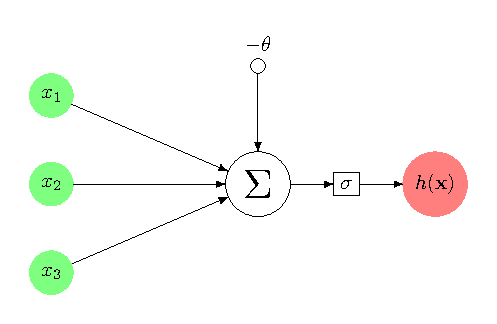
\includegraphics[width=.45\textwidth]{neuron-mp}
  \caption{Neurona McCulloch-Pitts con entrada $\textbf{x}$ y umbral $\theta$.}
  \label{fig:neuron-mp}
\end{figure}

\subsection{Perceptrón}

Con este modelo es posible representar alguna función muy sencilla pero no es útil para aprender funciones con un poco más de complejidad (observamos que el modelo está determinado por $\theta$, un único parámetro libre). Por ello surge una generalización de este modelo llamado el \textbf{perceptrón} \cite{rosenblatt1958perceptron}.

Este modelo incorpora una novedad fundamental: \textbf{pesos} que afectan a las entradas para regular las relaciones y las intensidades de estas. Al establecer conexiones más complejas entre las entradas se consigue que la neurona pueda aprender funciones que no sean tan simples como ocurría con la neurona de McCulloch-Pitts. También se admiten ahora las entradas reales, aumentando el dominio de entrada.

Definimos el perceptrón en \autoref{def:perceptron} y representamos visualmente en \autoref{fig:perceptron} viendo que lo que cambia simplemente son los pesos asociadas a las entradas, que actúan como reguladores de las conexiones.

\begin{definicion}[Perceptrón]
  Sea un vector de entrada $\textbf{x} \in \R^M$ con $M \in \N$, un vector de pesos $\textbf{w} \in \R^n$ y $\theta \in \R$ el umbral de activación, el perceptrón calcula la función $h$ dada por la siguiente expresión:
  $$h(\textbf{x}) = \sigma\left(\sum \limits^M_{i = 1}w_i x_i - \theta\right),$$
  donde $\sigma$ es la función de activación dada por $$\sigma(t) = \begin{cases} 1, \text{ si } t \geq 0, \\ 0, \text{ si } t < 0. \end{cases}$$
  \label{def:perceptron}
\end{definicion}

\begin{figure}[htpb]
  \centering
  %\hspace*{-2.5cm}
  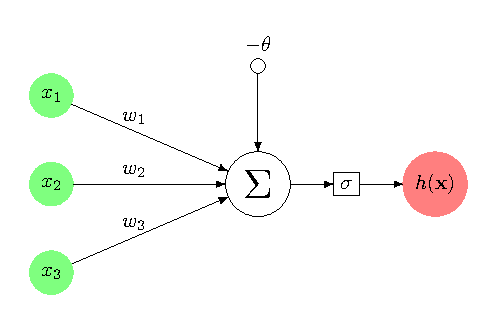
\includegraphics[width=.45\textwidth]{perceptron}
  \caption{Perceptrón con entrada $\textbf{x}$, pesos $\textbf{w}$ y umbral $\theta$.}
  \label{fig:perceptron}
\end{figure}

Considerando $\textbf{x} = (x_1, \ldots, x_M, 1)^T$ y $\textbf{w} = (w_1, \ldots, w_M, -\theta)^T$ podemos compactar la expresión, teniendo entonces $h(\textbf{x}) = \sigma(\textbf{w}^T \textbf{x})$. Observando detenidamente esta expresión vemos que lo que se tiene realmente es un modelo lineal: un \textbf{hiperplano} de $\R^{M}$ al que luego se le aplica una función no lineal.

Sabemos que un hiperplano divide $\R^{M}$ en dos regiones conexas, de manera que la función no lineal lo que está realizando realmente es asignar a cada región un valor distinto. Esta idea tan simple de funcionamiento nos permite pensar que el perceptrón sea capaz de solucionar \textbf{problemas de clasificación binarios}  (\autoref{def:clasbin}).

Estos problemas consisten fundamentalmente en inferir la relación que existe entre los datos de unas variables o \textbf{características} y las \textbf{etiquetas} asociadas a cada dato, que se identifican con una de las dos clases $+1$ o $-1$. Esta relación es la \textbf{función de etiquetado} desconocida $f$ que deseamos aprender, donde sabemos cómo se comporta en una \textbf{muestra} dada y que usaremos para que los modelos puedan aprender una función aproximada $h$. El objetivo entonces se convierte en conseguir que $h \approx f$ (ya veremos adelante como medimos esto).

Como nota adicional si consideramos la muestra extraída $(X, \textbf{y})$, podemos notar que $X \in \mathcal{M}_{N \times M}(\R)$ e $\textbf{y} \in \mathcal{M}_{N \times 1}(\N)$ y que
$$ X = \begin{bmatrix} \textbf{x}_1^T \\ \textbf{x}_2^T \\ \vdots \\ \textbf{x}_N^T \end{bmatrix}, \textbf{y} = \begin{bmatrix} y_1 \\ y_2 \\ \vdots \\ y_{N} \end{bmatrix}.$$

\begin{definicion}[Problema de clasificación binario]
  Sea $M \in \N$ el número de características, y $N \in N$ el número de observaciones, consideramos el espacio $\mathcal{X} \times Y \subseteq R^M \times \{-1, +1\}$ del que obtenemos una muestra $(X, \textbf{y}) \in \mathcal{X}^N \times Y^N$ que sigue una distribución de probabilidad $\mathcal{P}$ desconocida y el espacio de funciones del modelo dado $\mathcal{H}$. El problema consiste en encontrar un $h \in \mathcal{H}$ de tal manera que $h \approx f$, siendo $f$ la función de etiquetado:
  \begin{align*}
    f : \mathcal{X} & \to Y \\
    \textbf{x} & \mapsto f(\textbf{x}) \in \{-1, +1\}.
  \end{align*}
  \label{def:clasbin}
\end{definicion}

Sin más que cambiar los valores de la función de activación $\sigma$ de $\{0, 1\}$ a $\{-1, +1\}$ el perceptrón es capaz de aprender funciones capaces de solucionar estos problemas. De hecho, generalmente en el perceptrón se adopta en vez de la función $\sigma$ anteriormente comentada, la función $\sign$.

Podemos ver que el problema de clasificación binaria es equivalente a encontrar una función que separe dos conjuntos de datos agrupados por la clase, es decir a la separabilidad de dos conjuntos, que es lo que está haciendo el hiperplano $\textbf{w}$ del perceptrón (\autoref{fig:perceptron-ej} \cite{wikipedia2017separ}).

\begin{figure}[htpb]
  \centering
  %\hspace*{-2.5cm}
  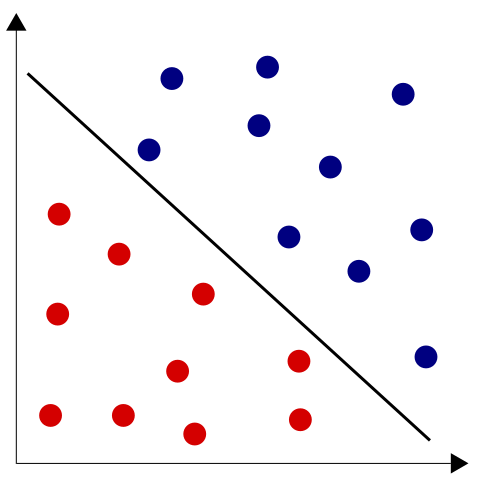
\includegraphics[width=.3\textwidth]{separabilidad}
  \caption{Ejemplo de perceptrón separando linealmente dos conjuntos de datos. Al separar es posible asignar a cada región una etiqueta, siendo equivalente separar a clasificar.}
  \label{fig:perceptron-ej}
\end{figure}

Gracias al Teorema de Convergencia del Perceptrón \cite{novikoff1963convergence} tenemos un resultado fuerte sobre la clase de funciones que puede aprender el perceptrón: se prueba que el modelo es capaz de aprender siempre una función $h$ que separa perfectamente dos conjuntos de datos que sean linealmente separables. Es decir, el perceptrón encuentra una solución muy buena $h \approx f$ ya que coinciden completamente, al menos en la muestra obtenida.

Mediante el \textbf{proceso de aprendizaje} se consigue que el modelo aprenda la función $h$ que buscamos. Este proceso es un método que tiene cada modelo de usar la información de la muestra recogida para poder aprender la función de etiquetado, que en el caso del perceptrón será una simple regla que actualiza los pesos por cada dato de la muestra, dada por
\begin{equation*}
  \textbf{w}_{(t + 1)} =
  \begin{cases}
    \textbf{w}_{(t)}, & \text{si } \sign(\textbf{w}^T_{(t-1)} \textbf{x}_t) \neq y_t, \\
    \textbf{w}_{(t)} + y_t \textbf{x}_t, & \text{en caso contrario.}
  \end{cases}
  \label{eq:percep-rule}
\end{equation*}

A pesar de todo, en cuanto los datos dejan de ser linealmente separables el perceptrón no tiene por qué converger siquiera a una solución. Si bien se puede arreglar quedándose con la mejor solución hasta el momento, las soluciones encontradas no suelen ser muy buenas. Por esta razón se necesitaba encontrar una manera de mejorar este modelo.

\subsection{Perceptrón MultiCapa}

Basándonos \cite{abu2012learning} explicaremos el proceso lógico que se lleva a cabo para poder aumentar la potencialidad del modelo del perceptrón.

Consideremos la siguiente función de la figura (\autoref{fig:xor}, \cite{abu2012learning}) que es bastante simple aunque la función $f$ no se puede aprender con un solo perceptrón (tomando una muestra se ve que los datos no son separables).

\begin{figure}[htpb]
  \centering
  %\hspace*{-2.5cm}
  \includegraphics[width=.35\textwidth]{XOR}
  \caption{Esta $f$ no se puede aprender con un solo perceptrón.}
  \label{fig:xor}
\end{figure}

Usemos dos perceptrones que aprendan cada uno de los hiperplanos separadores (\autoref{fig:dos-percep}, \cite{abu2012learning}) y fijémonos en las áreas de las clases. La función $f$ tiene la clase $+1$ cuando $h_1$ y $h_2$ tienen $(+1, -1)$ ó $(-1, +1)$; y la clase $-1$ cuando $(+1, +1)$ ó $(-1, -1)$. Este comportamiento es análogo a la función booleana $XOR$, por lo que podemos representarla como si lo fuera en base a las salidas de $h_1$ y $h_2$ ($f = XOR(h_1, h_2)$) siendo $+1$ \emph{Verdadero} y $-1$ \emph{Falso}. Usando notación booleana podemos reescribir $f = h_1\overline{h_2} + \overline{h_1}h_2$.

\begin{figure}[htpb]
  \centering
  %\hspace*{-2.5cm}
  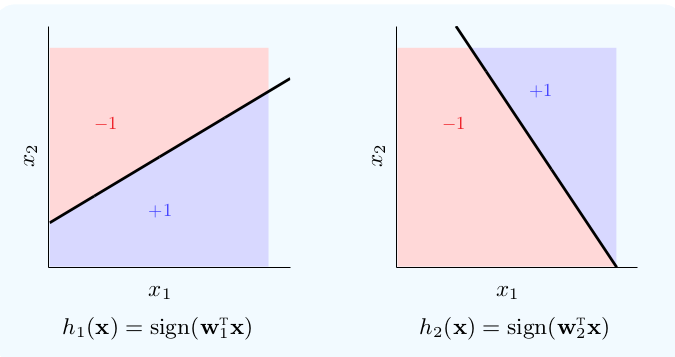
\includegraphics[width=.7\textwidth]{dospercep}
  \caption{Cada perceptrón aprende un hiperplano distinto.}
  \label{fig:dos-percep}
\end{figure}

Como estamos usando funciones $OR (+)$ y $AND (\cdot)$ para obtener $f$, el siguiente paso lógico es intentar expresar estas funciones como perceptrones. Es fácil ver que podemos obtenerlas de la siguiente manera
\begin{align*}
  AND(h1, h2) = \sign(h1 + h2 + 1.5), \\
  OR(h1, h2) = \sign(h1 + h2 - 1.5). \\
  \label{eq:and-or}
\end{align*}

Representamos estas funciones en forma de perceptrones, considerando la forma compacta ($\textbf{x} = (x_1, \ldots, x_M, 1)$, $\textbf{w} = (w_1, \ldots, x_M, -\theta)$ que ya habíamos comentado con la Neurona de McCulloch-Pitts (\autoref{fig:and-or}, \cite{abu2012learning}).

\begin{figure}[htpb]
  \centering
  %\hspace*{-2.5cm}
  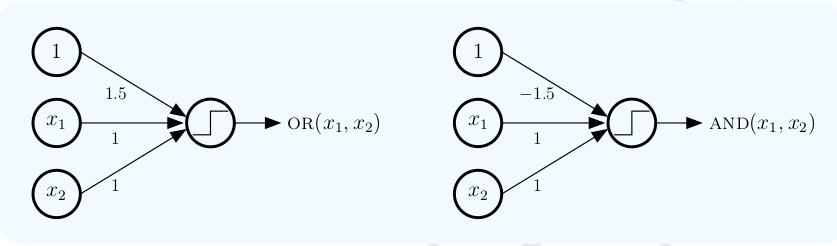
\includegraphics[width=.8\textwidth]{and-or}
  \caption{Funciones $AND$ y $OR$ como perceptrones.}
  \label{fig:and-or}
\end{figure}

Usando estos perceptrones podemos ir implementando poco a poco la función $f$: primero nos encontramos con una $OR$ que tiene como entradas $h_1\overline{h_2}$ y $\overline{h_1}h_2$ (\autoref{fig:or1}, \cite{abu2012learning}).

\begin{figure}[htpb]
  \centering
  %\hspace*{-2.5cm}
  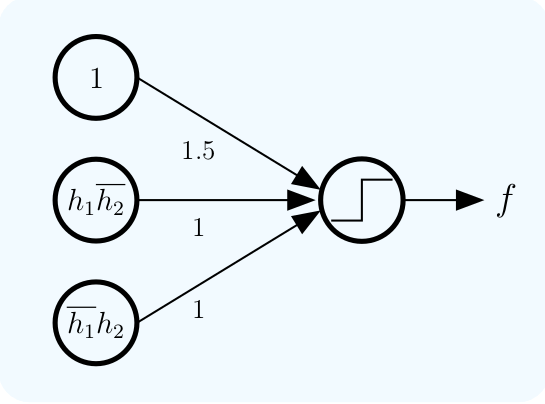
\includegraphics[width=.35\textwidth]{or1}
  \caption{Perceptrón que implementa $AND(h_1\overline{h_2}, \overline{h_1}h_2)$.}
  \label{fig:or1}
\end{figure}

Ahora tendríamos que usar dos perceptrones $AND$ para implementar $h_1\overline{h_2}$ y $\overline{h_1}h_2$. Como ambos perceptrones usarán la misma entrada ($\textbf{h} = (h_1, h_2, 1)$) se pueden representar los dos a la vez mediante dos vectores de pesos distintos (que son lo que determinan al perceptrón). Finalmente hay que tener en cuenta la negación de las entradas que se puede conseguir fácilmente cambiando el signo del peso asociado (\autoref{fig:and2}, \cite{abu2012learning}).

\begin{figure}[htpb]
  \centering
  %\hspace*{-2.5cm}
  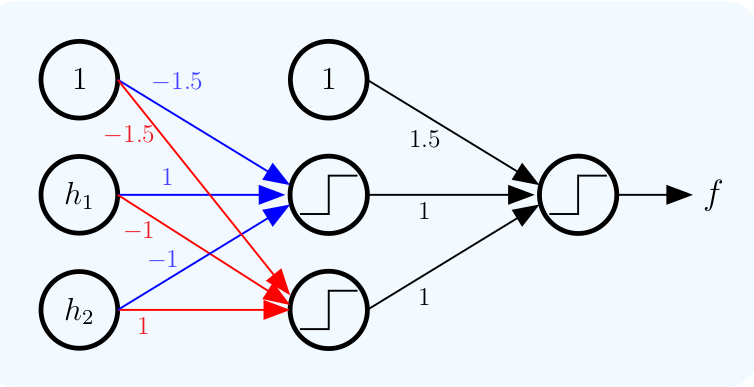
\includegraphics[width=.55\textwidth]{and2}
  \caption{Añadimos dos perceptrones $AND(h_1, \overline{h_2})$ (en azul) y $AND(\overline{h_1}, h_2)$ (en rojo).}
  \label{fig:and2}
\end{figure}

Falta obtener $h_1$ y $h_2$, pero si recordamos que se tenía que $h_1 = \sign(\textbf{w}^T_1 \textbf{x})$ y $h_2 = \sign(\textbf{w}^T_2 \textbf{x})$ que eran los dos perceptrones iniciales. Los incorporamos a nuestro esquema que ya estaría completo (\autoref{fig:mlp}, \cite{abu2012learning}).

\begin{figure}[htpb]
  \centering
  %\hspace*{-2.5cm}
  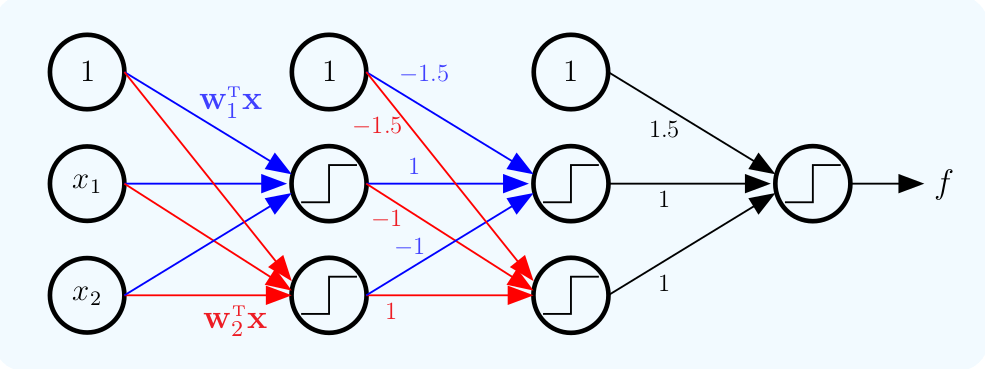
\includegraphics[width=.65\textwidth]{mlp}
  \caption{Los dos perceptrones iniciales $h_1$ (azul) y $h_2$ (rojo).}
  \label{fig:mlp}
\end{figure}

Analizando este modelo vemos que ha sido formado juntando perceptrones, uniendo las salidas de uno con la entrada de otro como si añadiésemos una \textbf{capa} tras otra de perceptrones. Debido a esto, este modelo se conoce como el \textbf{Perceptrón MultiCapa} (\emph{MultiLayer Perceptron}, MLP) \cite{rumelhart1985learning} y es de hecho la primera estructura de red neuronal básica y sobre la que se vertebrará toda la estructura del aprendizaje profundo.

\section{Redes Neuronales Hacia Adelante}

\subsection{Descripción}

Estudiamos las \textbf{redes neuronales hacia delante} (\emph{feedforward neural networks}, FFNN) que son las estructuras de redes neuronales más básicas y funcionales, donde sus procesos de funcionamiento y aprendizaje son el núcleo central de las redes neuronales, por lo que al estudiarlos en detalle nos permitirán entender \emph{a grosso modo} cualquier arquitectura utilizada actualmente.

Como hemos visto, este modelo surge con el perceptrón multicapa que se puede considerar un caso particular de esta aunque también se puede denominar como el mismo tipo de red. Usaremos como base los resultados y explicaciones de \cite{abu2012learning} para detallar exhaustivamente comentando su estructura, algoritmos de cómputo y aprendizaje.

\begin{figure}[htpb]
  \centering
  %\hspace*{-2.5cm}
  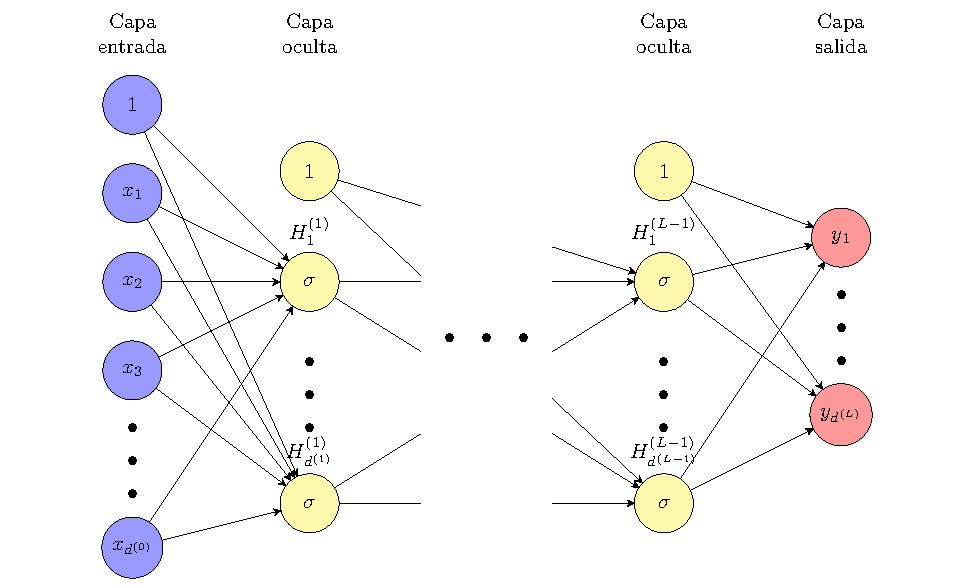
\includegraphics[width=1.\textwidth]{ffnn}
  \caption{Estructura genérica de una FFNN con $L$ capas, dimensiones $d^{(\ell)}$, entrada $\textbf{x}$, salida $\textbf{y}$ y funciones de activación $\sigma$.}
  \label{fig:ffnn}
\end{figure}

\subsection{Estructura}

\subsubsection{Arquitectura}

Veamos primero una estructura general de ejemplo en \autoref{fig:ffnn}. Consideramos una red con $L$ capas, etiquetadas con $\ell = 0, 1, \ldots, L$ donde $\ell = 0$ se corresponde con la capa de \textbf{entrada}, de las variables, que no se suele contar como una capa propia por lo que cuando se dice que una red tiene $L$ capas estamos diciendo que tiene $L-1$ capas intermedias ($0 < \ell < L$), llamadas capas \textbf{ocultas} y la capa $\ell = L$ de \textbf{salida} que es el resultado de la red.

Cada capa tiene una dimensión concreta, que denotaremos por $d^{(\ell)}$ y que indica que la capa $\ell$ tiene $d^{(\ell)} + 1$ nodos o neuronas (incluimos el nodo 1 del sesgo $\theta$) excepto para la capa de salida que se puede obviar. En particular se tiene que $d^{(0)} = M$, el número de variables y que $d^{(L)}$ será la dimensión de la salida, que ya no tiene que ser obligatoriamente un único nodo; de hecho, la salida ya no tiene que tomar valores discretos ya que podemos considerar otras funciones de activación que veremos un poco más adelante.

Observando este diagrama en profundidad notamos que cada neurona de una capa estará conectada por un peso (las conexiones) a todas las neuronas de la siguiente capa, formándose una red \textbf{densa}, nombre por la que también se suele conocer este tipo de capa. Esta estructura de conexiones de entrada a salida, capa por capa, es lo que le da nombre a este tipo de red puesto que los resultados se van pasando \emph{hacia adelante} siempre.

Adicionalmente, tengamos que en cuenta que si cada neurona está asociada con unos pesos, toda la capa $\ell$ que está formada por $d^{(\ell)}$ (sin contar la de sesgo) estará determinada por todos los pesos de cada neurona, que podemos representar como una matriz de la siguiente manera
\begin{equation*}
  W^{(\ell)} = \begin{bmatrix} \textbf{w}^{(\ell)}_{1} \ldots \textbf{w}^{(\ell)}_{d^{(\ell)}} \end{bmatrix} \in \mathcal{M}_{(d^{(\ell - 1)} + 1) \times d^{(\ell)}}(\R).
  \label{eq:pesos}
\end{equation*}

\subsubsection{Función de activación}

Respecto las funciones de activación $\sigma$, también llamadas funciones \textbf{de transformación} ya que son funciones no lineales, se deja de usar la función $\sign()$ en las capas ocultas debido a su discontinuidad en pos de otras funciones aproximadas más \emph{suaves} que realizan una función igual o muy parecida; las más famosas y usadas son las siguientes (funciones dibujadas \autoref{fig:activations}, \cite{moujahid2016activations}):

\begin{enumerate}
  \item Sigmoide: $$\sigma(x) = \dfrac{1}{1 + e^{-x}}.$$
  \item Tangente hiperbólica: $$\tanh(x) = \dfrac{e^x-e^{-x}}{e^{x}+e^{-x}}.$$
  \item ReLU (REctifier Linear Unit): $$ReLU(x) = x^+ = max(0, x).$$
\end{enumerate}

\begin{figure}[htpb]
  \centering
  %\hspace*{-2.5cm}
  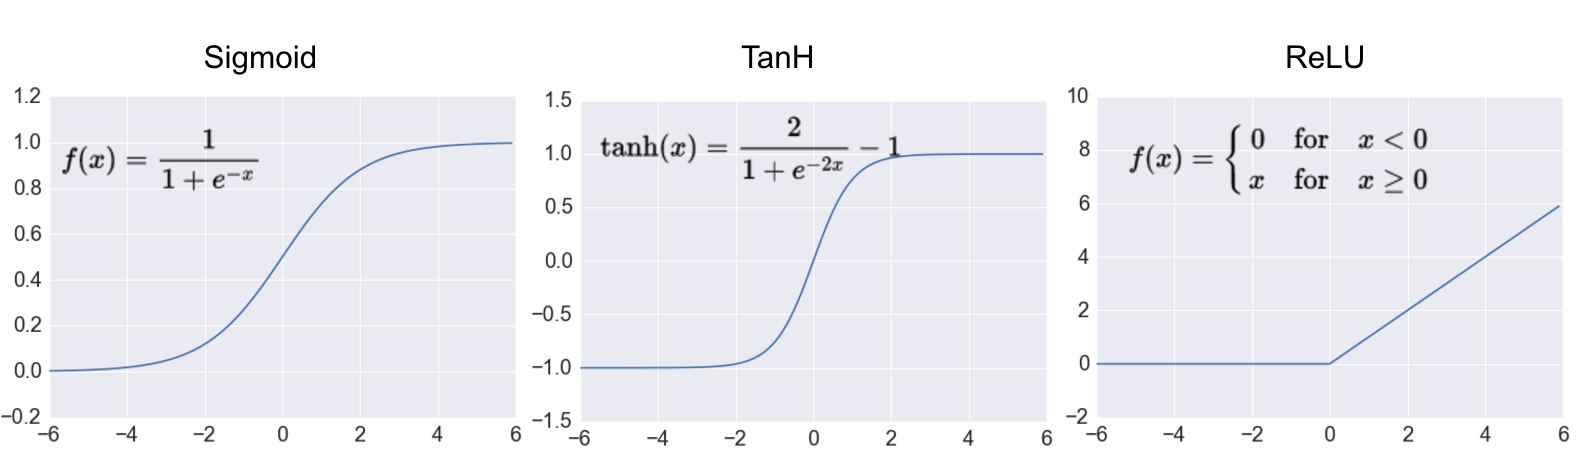
\includegraphics[width=1.\textwidth]{activations}
  \caption{Funciones de activación.}
  \label{fig:activations}
\end{figure}

Donde sí podremos usar $\sign()$ será en la capa de salida cuando queramos obtener un resultado respecto una clase, sin embargo recordemos que ahora podemos tener una dimensión de salida cualquiera y no estamos limitados a aprender funciones discretas. De hecho, si consideramos otras capas de activación para la salida podemos aprender distintos tipos de funciones según el problema que tengamos entre manos.

Por ejemplo, para los problemas de \textbf{regresión} que son simplemente problemas de clasificación donde la $f$ pasa de ser discreta a continua ($f: \mathcal{X} \to Y$, $Y \subseteq \R^n$) podemos usar directamente la función identidad ($f(x) = x$); para los problemas de \textbf{regresión logística}, que considera una función que en vez de asignar una clase directamente asigna la \textbf{probabilidad} ($\mathcal{X} \to Y$, $Y \subseteq [0, 1]$), se puede usar la función $\tanh()$ o \emph{sigmoide}.

De hecho, cuando tenemos un problema de clasificación con $n$ clases en vez de calcular una clase directamente se calcula la probabilidad \textbf{asociada} a cada clase y cuando se hace una clasificación de una única clase se toma la de mayor probabilidad. Esto es posible utilizando en la capa de salida la función de activación \textbf{softmax} \autoref{def:softmax}, que toma un vector real de tamaño $n$ y lo normaliza en una distribución de probabilidad.

\begin{definicion}[Softmax]
  La función softmax es una función $\sigma : \R^n \to \R^n$ definida de la siguiente forma:
  $$\sigma(\textbf{x}) = \sum \limits^n_{i = 1} e^{x_i} \begin{pmatrix} e^{x_1} \\ \vdots \\ e^{x_n}\end{pmatrix}.$$
  \label{def:softmax}
\end{definicion}

En cualquier caso, el modelo $\mathcal{H}_{nn}$ queda determinado por la \textbf{arquitectura} de la red neuronal, es decir, especificar el número de capas y la dimensión de cada capa: fijar $L$ y $\textbf{d} = [d^{(0)}, d^{(1)}, \ldots, d^{(L)}]$. Por tanto cada función de hipótesis $h \in \mathcal{H}_{nn}$ estará representada por los pesos de las conexiones entre las capas que representaremos con matrices: $\textbf{W} = \{W^{(1)}, W^{(2)}, \ldots, W^{(L)}\}$.

\subsection{Propagación hacia adelante}

Antes de explicar el algoritmo de cálculo de $h(\textbf{x})$, indiquemos una breve notación: sea $\ell \in \{1, 2, \ldots, L\}$, consideramos la capa $\ell$ que recibe el el resultado $\textbf{s}^{(\ell)} \in \mathcal{M}_{d^{(\ell)} \times 1}(\R)$ de la multiplicación de la capa anterior mediante la expresión
\begin{equation*}
  \textbf{s}^{(\ell)} = (W^{(\ell)})^T \textbf{x}^{(\ell-1)},
  \label{eq:fp1}
\end{equation*}
usando los datos de entrada $\textbf{x}^{(\ell-1)} \in \mathcal{M}_{(d^{(\ell-1)} + 1) \times 1}(\R)$ con la matriz de pesos $W^{(\ell)} \in \mathcal{M}_{(d^{(\ell-1)} + 1) \times d^{(\ell)}}(\R)$ a los que le aplica la función de activación $\sigma$ obteniendo la salida $\textbf{x} \in \mathcal{M}_{d^{(\ell) \times 1}}(\R)$ dada por
\begin{equation*}
  \textbf{x}^{(\ell)} = \begin{bmatrix} 1 \\ \sigma(\textbf{s}^{(\ell)})\end{bmatrix}.
  \label{eq:fp2}
\end{equation*}

La \textbf{propagación hacia adelante} (\emph{forward propagation}) es el algoritmo para poder calcular el resultado de la red $h(\textbf{x})$. A partir de los datos de entrada $\textbf{x}^{(0)}$ se calcula la siguiente salida de la capa que se \textbf{propaga} a la siguiente capa y así hasta llegar al final siguiendo la siguiente cadena
\begin{equation}
  \textbf{x} = \textbf{x}^{(0)} \xrightarrow[]{W^{(1)}} \textbf{s}^{(1)} \xrightarrow[]{\sigma} \textbf{x}^{(1)} \xrightarrow{W^{(2)}} \ldots \xrightarrow{\sigma} \textbf{x}^{(L)} = h(\textbf{x}).
  \label{eq:cadena-fp}
\end{equation}

Formalizamos este proceso mediante el algoritmo \autoref{alg:fp} \cite{abu2012learning}. Aunque en principio solo necesitamos la última salida $h(\textbf{x}) = \textbf{x}^{(L)}$ devolvemos todas las entradas $\textbf{x'}$ y salidas $\textbf{s}$ ya que los necesitaremos más adelante.

\begin{algorithm}[htbp]
\SetAlgoLined
 \tcp{Inicializamos con la entrada}
 $\textbf{x}^{(0)} \gets \textbf{x}$\;
 \tcp{Propagamos para cada capa}
 \For{$\ell = 1, \ldots, L$} {
  \tcp{Calculamos la entrada de la capa}
  $\textbf{s}^{(\ell)} \gets (W^{(\ell)})^T \textbf{x}^{(\ell - 1)}$\;
  \tcp{Se devuelve la salida de la capa}
  $\textbf{x}^{(\ell)} \gets \begin{bmatrix} 1 \\ \sigma(\textbf{s}^{(\ell)})\end{bmatrix}$\;
 }
 \tcp{Devolvemos las entradas y salidas}
 $\textbf{x'} \gets \left[\textbf{x}^{(0)}, \ldots, \textbf{x}^{(L)}\right]$\;
 $\textbf{s} \gets \left[\textbf{s}^{(1)}, \ldots, \textbf{s}^{(L)}\right]$\;
 \KwResult{$\textbf{x'}$, $\textbf{s}$}
 \caption{$ForwardPropagation(\textbf{x})$)}
 \label{alg:fp}
\end{algorithm}

\subsection{Descenso en gradiente}

Lo último que nos falta para poder empezar a usar estos modelos es un mecanismo de aprendizaje, el algoritmo para que la red pueda aprender la función $f$ mediante la muestra de datos que tenemos, es decir buscar una $h \in \mathcal{H}_{nn}$ tal que $h \approx f$, o lo que es lo mismo $h(\textbf{x}) \approx f(\textbf{x}), \; \forall \textbf{x} \in \mathcal{X}$.

Está claro que cuanto más se aproxime $h$ a $f$ mejor será, aunque necesitamos una manera de formalizar esta similitud para poder trabajarla. Recordemos que tenemos una muestra que podemos suponer que es suficientemente grande y representativa de la distribución subyacente que se puede usar para poder valorar la diferencia entre $h$ y $f$. La idea que surge es valorar con una función de \textbf{error} o \textbf{pérdida} las diferencias entre $f$ y $h$ para todos los valores de la muestra, dando un valor indicativo con el que podemos trabajar.

Este tipo de funciones generalmente son de la forma $E_{\mathcal{D}} : \mathcal{H} \to \R^+_0$ que toman una función del conjunto de hipótesis del modelo y se valora en base a un criterio impuesto según el problema que se quiera resolver usando la muestra $\mathcal{D}$; por ejemplo para problemas de regresión uno querría usar el conocido \textbf{error cuadrático medio}. Fijando una función de error, como queremos la función $h$ que menor $E_{\mathcal{D}}(h)$ tenga el problema de aprendizaje se ha convertido en un problema de \textbf{minimización}, teniendo en cuenta que para que la función sea de variable real tomaremos la representación de $h$ por los pesos $\textbf{w}$ (veremos cómo extenderlo a $\textbf{W}$).

Es importante entender que se puede imponer una función de error para minimizar en un modelo pero que luego el problema original que se quiere resolver sea distinto, de manera que la \textbf{valoración} del modelo se realizará de otra manera; concretamente usaremos las \textbf{métrica} para valorar la bondad de los modelos, que veremos con detalle más adelante en \autoref{ch:metricas}.

Nuestro problema de aprendizaje se ha convertido en un problema de minimización donde para resolverlo podemos recurrir a los métodos numéricos existentes como el \textbf{Descenso en Gradiente} (\emph{Gradient descent}, GD). \cite{curry1944method}.

El descenso en gradiente (\autoref{def:gd}) es un método de minimización cuya idea principal se basa en ir moviéndose hacia el mínimo \emph{bajando} poco a poco tomando la dirección contraria (negativa) del gradiente (\autoref{fig:gd}, \cite{molala2019sd}). Como la dirección del gradiente indica donde aumenta la función localmente, al tomar la dirección contraria después de suficientes iteraciones, esperamos idealmente llegar al menos a un mínimo local (pudiera acabar en puntos de silla) aunque lo deseable será llegar al global si lo hubiera. Bajo ciertas condiciones podemos asegurar la convergencia de este método, por ejemplo si la función es convexa y el gradiente es lipschiziano \cite{shalev2014understanding}.

\begin{figure}[htpb]
  \centering
  %\hspace*{-2.5cm}
  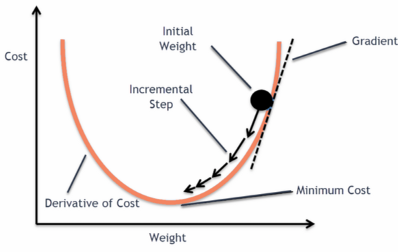
\includegraphics[width=.5\textwidth]{gd}
  \caption{Ejemplo del Descenso en Gradiente en una parábola.}
  \label{fig:gd}
\end{figure}

\begin{definicion}[Descenso en grandiente]
  Sea $E : \R^m \to \R$ una función diferenciable, un punto inicial $\textbf{w}_{(0)}$ y la tasa de aprendizaje $\mu \in \R^+$. El descenso en gradiente es un método iterativo de primer orden para encontrar mínimos que sigue la siguiente regla de actualización:
  $$\textbf{w}_{(t)} = \textbf{w}_{(t-1)} - \mu \nabla E(\textbf{w}_{(t-1)}), \; \forall t \in \N.$$
  \label{def:gd}
\end{definicion}

El establecer un valor para la \textbf{tasa de aprendizaje} (\emph{learning rate}) no es una tarea para nada trivial, de hecho en \autoref{fig:lr} podemos ver las implicaciones de no escoger una tasa adecuada: si es muy baja puede resultar en una convergencia \textbf{muy lenta}, y si es alta puede que \textbf{no converga} o lo haga saltándose mínimos \textbf{mejores}, también podría pasar que el error \emph{explote} (diverge) \cite{ruder2016overview}.

\begin{figure}[htpb]
  \centering
  %\hspace*{-2.5cm}
  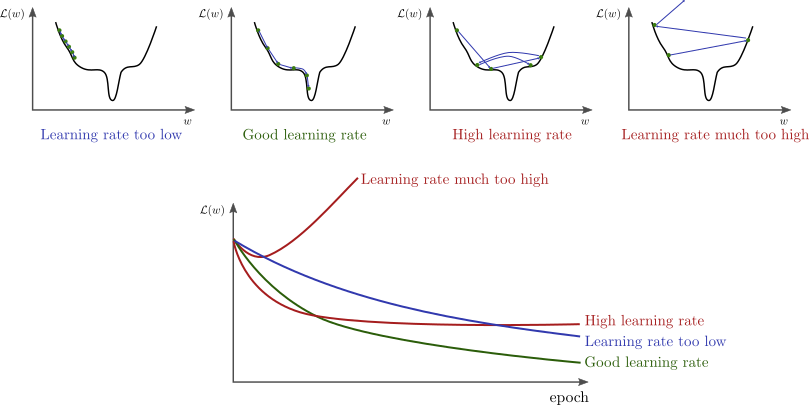
\includegraphics[width=.9\textwidth]{lr}
  \caption{Diferentes resultados según la tasa de aprendizaje $\mu$.}
  \label{fig:lr}
\end{figure}

En principio ya tendríamos un método para poder intentar que nuestra red pueda aprender pero tenemos un problema general a la hora de calcular $\nabla E_\mathcal{D}$: si nuestra muestra de datos $\mathcal{D}$ es muy grande esto puede provocar que el cálculo sea muy costoso en tiempo e incluso supere los tamaños de memoria del \emph{hardware} y esto solo para un paso, por lo que para realizar las múltiples iteraciones necesarias para la convergencia resulte completamente inviable \cite{ruder2016overview}.

La solución a esto la aporta el \textbf{Descenso en Gradiente Estocástico} (\emph{Stochastic Gradient Descent}, SGD) \cite{robbins1951stochastic} que es igual que el Descenso en Gradiente, solo que en vez de tomar todo el conjunto de datos de golpe $\mathcal{D}$ se hace una partición en subconjuntos de tamaño $n$ llamados \textbf{lotes} o \emph{batches} y se actualizan los pesos para cada \emph{batch}. La aleatoriedad que se introduce al escoger los \emph{batches} es interesante ya que nos puede ayudar en la búsqueda de mínimos, aportándonos un poco de exploración para encontrar mejores mínimos en la función.

Técnicamente se llama SGD cuando $n=1$, es decir, cuando actualizamos la red dato a dato, cuando $1 < n < N$ se suele llamar al método \textbf{Descenso en Gradiente con Mini-lotes} (\emph{Mini-batch Gradient Descent}) aunque también se usa SGD indistintivamente.

Respecto al tamaño del \emph{batch} $n$, el rango de valores típico de suele estar en $[32, 256]$ aunque dependerá del modelo y problema concretos que se esté considerando, se suele probar con los valores típicos y se van adaptando para obtener un buen funcionamiento.

En principio ya estaríamos listos para que nuestra red aprendiera, pero merece la pena mencionar que en la actualidad se utilizan métodos derivados más complejos que intentan mejorar el funcionamiento del SGD para una convergencia más rápida y encontrar mejores mínimos. Listamos unos cuantos de los más conocidos y populares: \textbf{Adadelta}, \textbf{RMSprop}, \textbf{Adam}, \textbf{AdaMax} y \textbf{Nadam} \cite{ruder2016overview}. No existe un método absoluto que gane a todos, de hecho SGD sigue siendo una opción viable, por lo que dependiendo del problema se puede decidir escoger uno y otro; aun así uno de los optimizadores más populares y que se suele escoger para las redes neuronales es \textbf{Adam}.

\subsection{Propagación hacia atrás}

\subsubsection{Sensibilidades}

Vamos a aplicar SGD para que nuestro modelo aprenda, para ello necesitamos $\nabla E_{\mathcal{D}} (\textbf{w})$ pero aquí $\textbf{w} = \{W^{(1)}, \ldots, W^{(L)}\}$ por lo que hay que calcular las derivadas parciales respecto \textbf{todas las matrices}. Considerando que el error en la muestra no es más que la media de los errores de cada dato podemos reescribir como
\begin{equation*}
  E_{\mathcal{D}}(\textbf{w}) = \dfrac{1}{N} \sum \limits_{d \in \mathcal{D}} E_d(\textbf{w}) = \dfrac{1}{N} \sum \limits^N_{i = 1} e_i.
  \label{eq:esample}
\end{equation*}

Por tanto las derivadas parciales del error respecto cada matriz de $\textbf{w}$ serán como
\begin{equation*}
  \dfrac{\partial E_{\mathcal{D}}}{\partial W^{(\ell)}} = \dfrac{1}{N} \sum \limits^N_{i = 1} \dfrac{\partial e_i}{\partial W^{(\ell)}}.
  \label{eq:ederiv}
\end{equation*}

Es posible usar métodos numéricos para obtener cada $\dfrac{\partial e}{\partial W^{(\ell)}}$ pero la complejidad del algoritmo para la derivada respecto cada peso sería de $O(Q^2)$ siendo $Q$ el número de pesos, que se hace computacionalmente inviable. Surge así el algoritmo de la \textbf{propagación hacia atrás} (\emph{backpropagation}) que nos permite calcular estas derivadas eficientemente con una complejidad de $O(Q)$.

Este algoritmo se basa en la \textbf{regla de la cadena} para expresar las derivadas parciales de la capa $\ell$ en base a las de la capa $(\ell + 1)$. Para describir el funcionamiento, definamos primero el \textbf{vector de sensibilidad} (\autoref{def:sensibilidad}) que trata de medir como cambia $e$ respecto $\textbf{s}^{\ell}$.

\begin{definicion}[Vector de sensibilidad]
  Sea $\ell \in \N$, el vector de sensibilidad de la capa $\ell$ notado por $\pmb{\delta}^{(\ell)}$, es el gradiente del error $e$ respecto la señal de entrada en la capa $\textbf{x}^{(\ell)}$, es decir:
  $$\pmb{\delta}^{(\ell)} = \dfrac{\partial e}{\partial \textbf{s}^{(\ell)}}.$$
  \label{def:sensibilidad}
\end{definicion}

Usando la regla de la cadena, y recordando que $\textbf{s}^{(\ell)} = (W^{(\ell)})^T \textbf{x}^{(\ell-1)}$ expresamos las derivadas parciales con la sensibilidad de la siguiente forma \cite{abu2012learning}
\begin{equation*}
  \dfrac{\partial e}{\partial W^{(\ell)}} = \dfrac{\partial e}{\partial \textbf{s}^{(\ell)}} \cdot \dfrac{\partial \textbf{s}^{(\ell)}}{\partial W^{(\ell)}} = \textbf{x}^{(\ell - 1)}(\pmb{\delta}^{(\ell)})^T.
  \label{eq:senpar}
\end{equation*}

Además, considerando que $\textbf{x}^{(\ell)} = \sigma(\textbf{s}^{(\ell)})$ y volviendo a aplicar la regla de la cadena podemos obtener la sensibilidad de la capa $(\ell)$ en función de la de $(\ell + 1)$ para cada coordenada
\begin{equation*}
  \delta_i^{(l)} = \dfrac{\partial e}{\partial s_i^{(l)}} =  \sum \limits^{d^{(\ell)}}_{j = 1} \left(\dfrac{\partial e}{\partial s_j^{(\ell + 1)}} \cdot \dfrac{\partial s_j^{(\ell + 1)}}{\partial x_i^{(\ell)}} \right) \cdot \dfrac{\partial x_i^{(\ell)}}{\partial s_i^{(\ell)}} = \sum \limits^{d^{(\ell)}}_{j = 1} \left(\delta^{(\ell)}_i w_{ij}^{(\ell)}\right) \sigma'(s_i^{(\ell)}),
  \label{eq:senpar2}
\end{equation*}
que extendemos al vector entero \cite{abu2012learning}
\begin{equation*}
  \pmb{\delta}^{(\ell)} = \sigma'(\textbf{s}^{(\ell)}) \otimes \left[W^{(\ell + 1)} \pmb{\delta}^{(\ell + 1)}\right]^{d^{(\ell)}}_1,
  \label{eq:senpar3}
\end{equation*}
donde $\otimes$ denota la multiplicación componente a componente y $\left[\empty\textbf{v}\right]^{d^{(\ell)}}_{1}$ indica que se toman las componentes $1, \ldots, d^{(\ell)}$ del vector $\textbf{v}$ que simplemente indica que no contamos la componente del nodo de sesgo (el nodo 1).

Recapitulando: las salidas $\textbf{x}^{(\ell)}$ se pueden obtener simplemente calculando el resultado de la red (propagación hacia adelante), lo que resta por calcular son las sensibilidades $\pmb{\delta}^{(\ell)}$. Replicamos el algoritmo de la propagación hacia adelante con modificaciones: en vez de ir obteniendo y propagando las salidas hacia adelante (se usa $\textbf{x}^{(\ell)}$ para $\textbf{x}^{(\ell + 1)}$), lo haremos con las sensibilidades propagándolas \emph{hacia atrás} (se usa $\pmb{\delta}^{(l+1)}$ para $\pmb{\delta}^{(\ell)}$).

Empezaremos calculando $\pmb{\delta}^{(L)}$ directamente con la definición y después iremos propagando hacia atrás las sensibilidades. Por ejemplo, si consideramos el error cuadrático medio con un modelo cuya salida sea un único valor tendríamos $e(\textbf{x}; h) = (h(\textbf{x}) - y)^2$ y podemos calcular la sensibilidad fácilmente como
\begin{equation*}
  \pmb{\delta}^{(L)} = \dfrac{\partial e}{\partial \textbf{s}^{(L)}} = \dfrac{\partial}{\partial \textbf{s}^{(L)}} (\textbf{x}^{(L)} - y)^2 = 2(\textbf{x}^{(L)} - y) \dfrac{\partial \textbf{x}^{(L)}}{\partial \textbf{s}^{(L)}} = 2(\textbf{x}^{(L)} - y)\sigma'(\textbf{s}^{(L)}).
  \label{eq:delta-ele}
\end{equation*}

Después habrá que calcular la derivada de la función de activación elegida, por ejemplo para $\sigma(s) = \tanh(s)$ tenemos que $\sigma'(\textbf{s}^{(L)}) = 1 - \sigma(\textbf{s}^{(L)})^2$; para la lineal (la identidad) $\sigma(\textbf{s}^{(L)}) = \textbf{s}^{(L)}$ se tendrá simplemente que $\sigma'(\textbf{s}^{(L)}) = 1$.

Describimos el método de \emph{backpropagation} por el cual calculamos las sensibilidades $\pmb{\delta}^{(\ell)}$ en \autoref{alg:bp}.

\begin{algorithm}[htbp]
\SetAlgoLined
 \tcp{Hacemos propagación hacia adelante para obtener $\textbf{x}$ y $\textbf{s}$}
 $\left[\textbf{x}^{(0)}, \ldots, \textbf{x}^{(L)}\right], \left[\textbf{s}^{(1)}, \ldots, \textbf{s}^{(L)}\right] \gets ForwardPropagation(\textbf{x})$\;
 \tcp{Inicializamos las sensibilidades}
 $\pmb{\delta} \gets \dfrac{\partial e}{\partial \textbf{s}^{(L)}}(\textbf{x}, y)$\;
 \tcp{Propagamos hacia atrás}
 \For{$\ell = L-1, \ldots, 1$} {
  \tcp{Calculamos la sensibilidad}
  $\pmb{\delta}^{(\ell)} \gets \sigma'(\textbf{s}^{(\ell)}) \otimes \left[W^{(\ell + 1)}\pmb{\delta}^{(\ell + 1)}\right]^{d^{(\ell)}}_1$
 }
 \tcp{Devolvemos las sensibilidades}
 $\pmb{\delta} \gets \left[\pmb{\delta}^{(1)}, \ldots, \pmb{\delta}^{(L)}\right]$\;
 \KwResult{$\pmb{\delta}$}
 \caption{$BackPropagation(\textbf{x}, y)$}
 \label{alg:bp}
\end{algorithm}

\subsubsection{Aprendizaje}

Por fin podemos definir el algoritmo SGD \autoref{alg:sgd-nn} por el cual podemos hacer que la red aprenda: solo necesitamos pasar como parámetros la muestra $(X, \textbf{y})$, la tasa de aprendizaje $\mu$ y el tamaño de los mini-\emph{batches} $tam_{batch}$. Obviamente se habrá fijado la arquitectura de la red junto a la función de error a minimizar y las funciones de activación.

\begin{algorithm}[htbp]
\SetAlgoLined
  \tcp{Inicializamos los pesos aleatorios}
  $\left[ W^{(1)}, \ldots, W^{(L)}\right] \gets PesosAleatorios()$\;
  \tcp{Iteramos hasta que se cumpla el criterio de parada}
  \Repeat{$CondicionParada()$}{
    \tcp{Dividimos aleatoriamente en mini-\emph{batches} de tamaño $tam_{batch}$}
    $n_{batches} \gets M \, // \, tam_{batch}$\;
    $\left[(X_{1}, \textbf{y}_1), \dots, (X_{n_{batches}}, \textbf{y}_{n_{batches}})\right] \gets ParticionAleatoria(X, \textbf{y})$\;
    \tcp{Por cada mini-\emph{batch} actualizamos los pesos}
    \For{$i = 1, \ldots, n_{batches}$}{
      \tcp{Inicializamos los gradientes a 0}
      $\left[G^{(\ell)}, \ldots, G^{(L)}\right] \gets 0 \cdot \left[W^{(1)}, \ldots, W^{(L)}\right]$\;
      \tcp{Calculamos el gradiente de todo el mini-\emph{batch}}
      \For{$(\textbf{x}, y) \in (X_{i}, \textbf{y}_i)$}{
        \tcp{Forwardpropagation y backpropagation}
        $\left[\textbf{x}^{(0)}, \ldots, \textbf{x}^{(L)}\right] \gets ForwardPropagation(\textbf{x})$\;
        $\left[\pmb{\delta}^{(1)}, \ldots, \pmb{\delta}^{(L)}\right] \gets BackPropagation(\textbf{x}, y)$\;
        \tcp{Actualizamos el gradiente de cada capa}
        \For{$\ell = 1, \ldots, L$}{
          $G^{(\ell)}(\textbf{x}) \gets \textbf{x}^{(\ell-1)}(\pmb{\delta}^{(\ell)})^T$\;
          $G^{(\ell)} \gets G^{(\ell)} + \dfrac{1}{tam_{batch}}G^{(\ell)}(\textbf{x})$\;
        }
      }
      \tcp{Actualizamos los pesos de cada capa}
      \For{$\ell = 1, \ldots, L$}{
        $W^{(\ell)} \gets W^{(\ell)} - \mu G^{(\ell)}$\;
      }
    }
  }
 \tcp{Devolvemos los pesos}
 $\textbf{w} \gets \left[ W^{(1)}, \ldots, W^{(L)}\right]$\;
 \KwResult{$\textbf{w}$}
 \caption{$AprendizajeRed(X, \textbf{y}, \mu, tam_{batch})$}
 \label{alg:sgd-nn}
\end{algorithm}

Esta es la base completa de las redes neuronales, las distintas arquitecturas que se han desarrollado a lo largo de los últimos años no cambian demasiado en los aspectos fundamentales por lo que sabiendo todo lo que hemos visto podemos hacernos una idea de cómo se extiende a los casos más complejos.

\subsection{Error y sobreajuste}

También tenemos que comentar que a la hora de entrenar las redes neuronales hay que tener en cuenta un aspecto fundamental en el aprendizaje automático: el \textbf{compromiso} entre el \textbf{sesgo} (\emph{bias}) y la \textbf{varianza} (\emph{variance}).

Cuando hablamos de sesgo estamos generalmente hablando del error del modelo en el conjunto de nuestra muestra, notado típicamente por $E_{in}$ y en principio es el error que queremos reducir en el proceso de aprendizaje de nuestros modelos. Sin embargo tenemos un problema, si intentamos ajustarnos perfectamente a los datos casi anulando efectivamente el sesgo pudiera ser que en otra muestra distinta de datos observemos que el modelo no ajusta bien estos nuevos datos.

Este efecto es el conocido \textbf{sobreajuste} (\emph{overfitting}) que se da cuando el error de entrenamiento $E_{in}$ no coincide (generalmente es mucho más bajo) con $E_{out}$ que es el error del modelo fuera de nuestra muestra. Este efecto ocurre debido al término de la \textbf{varianza} del error, que para nuestro modelo probablemente sea muy alta, y que nos indica generalmente el grado de variabilidad del error para una muestra distinta de datos.

Cuanto más queramos bajar el sesgo, más nos ajustaremos a los datos y provocaremos que aumente la varianza y por tanto tengamos sobreajuste; si no bajamos el sesgo a costa de no aumentar la varianza entonces el modelo pudiera estar mal ajustado (\emph{underfitting}). Tenemos que encontrar un \textbf{compromiso} entre ambos términos, un equilibrio adecuado para poder alcanzar un buen modelo que resuelva nuestro problema; podemos ver un ejemplo de lo que hablamos en una problema de regresión \autoref{fig:overfitting} \cite{bhande2018overfitting}.

\begin{figure}[htpb]
  \centering
  %\hspace*{-2.5cm}
  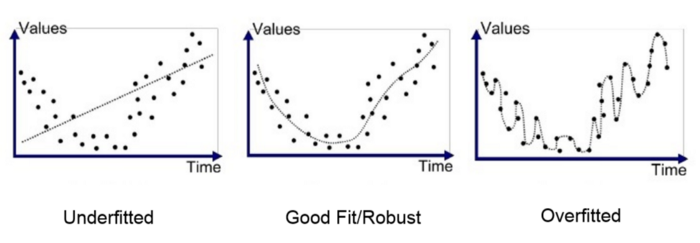
\includegraphics[width=.9\textwidth]{overfitting}
  \caption{Efecto del \emph{overfitting} y \emph{underfitting}.}
  \label{fig:overfitting}
\end{figure}

El proceso del sobreajuste está relacionado con la \textbf{complejidad} del modelo, que nos indica la capacidad del conjunto de hipótesis $\mathcal{H}$ para aprender funciones, siendo una medida común
la \textbf{Dimensión de Vapnik-Chervonenkis} (dimensión VC) $d_{VC}$ \cite{vapnik2015uniform}.  La idea principal es que cuanto más alta es esta dimensión, el modelo es capaz de aprender funciones más complejas y por tanto es capaz de ajustar bien los datos; sin embargo si la complejidad es mucho mayor que la de la función entonces es cuando se produce el efecto del sobreajuste.

Para evitar esto utilizamos técnicas de \textbf{regularización} que se encargan de imponer condiciones sobre el modelo reduciendo así el conjunto de hipótesis $\mathcal{H}$ considerado y disminuyendo su complejidad, que se traduce a un decremento de la varianza a costa de un pequeño aumento del sesgo.

Dentro de este campo hay muchas técnicas que podemos aplicar a las redes neuronales: reducción de la dimensión en profundidad y/o anchura, parada temprana (\emph{early stopping}) que trata de parar el entrenamiento bajo ciertas condiciones, \emph{dropout} \cite{hertz2018introduction, hinton2012improving} que desactiva aleatoriamente algunas neuronas de las capas mientras la red se entrena, o añadir términos de penalización al error (\emph{weight decay}) siendo los más conocidos la regularización L1 (Lasso)
\begin{equation*}
  E_{reg} = E_{in} + \dfrac{\lambda}{N} \sum \limits^{L}_{\ell = 1} ||W^{(\ell)}||_1, \; \lambda \in \R,
  \label{eq:l1}
\end{equation*}
y L2 \cite{krogh1992simple}
\begin{equation*}
  E_{reg} = E_{in} + \dfrac{\lambda}{N} \sum \limits^{L}_{\ell = 1} ||W^{(\ell)}||_2^2, \; \lambda \in \R.
  \label{eq:l2}
\end{equation*}

Para acabar, en las redes neuronales generalmente se deja una muestra de datos que no se usa para entrenar para obtener una estimación del error fuera de la muestra $E_{out}$ que se llama conjunto de \textbf{validación} $E_{val}$ o de \textbf{test} $E_{test}$ y que podemos usar para comprobar si tenemos sobreajuste o no. Si vamos dibujando $E_{in}$ y $E_{val}$ conforme vamos entrenando la red (cada época) podemos observar cuando hay sobreajuste y parar en ese momento (\autoref{fig:overfitting-nn} \cite{julien2018overfitting}).

\begin{figure}[htpb]
  \centering
  %\hspace*{-2.5cm}
  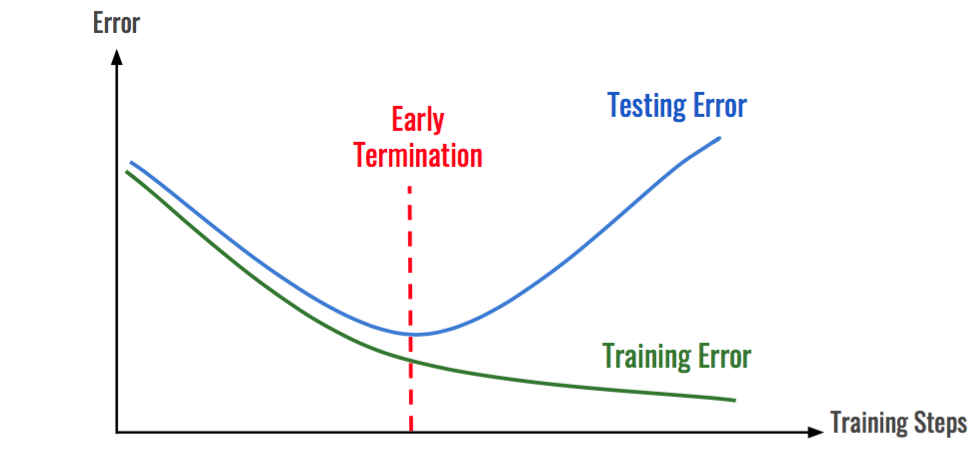
\includegraphics[width=.6\textwidth]{overfitting-nn}
  \caption{Sobreajuste entrenando una red neuronal, tenemos que parar antes de que las curvas diverjan.}
  \label{fig:overfitting-nn}
\end{figure}

\subsection{Teorema de aproximación universal}

Finalmente veamos un resultado matemático que nos permite afirmar con seguridad la fuerte capacidad de las redes neuronales para aprender funciones: el \textbf{teorema de aproximación universal}.

Este teorema tiene dos versiones: el caso de anchura indeterminada, que es la forma clásica, \cite{cybenko1989approximation} y el de profundidad indeterminada \cite{lu2017expressive}.

El caso de anchura arbitraria (\autoref{th:aproxuni-anchura}) nos dice que \textbf{cualquier función continua} en un subconjunto compacto de $R^k$ se puede aproximar con tanta precisión como se quiera con una red neuronal \emph{feed-forward} con una capa oculta y función de activación sigmoide aunque de anchura libre.

\begin{teorema}[Teorema de aproximación universal (anchura indeterminada)]
  Sea $\sigma : \R \to \R$ una función no constante, acotada y continua a la que llamamos función de activación, $I_n$ el hipercubo unidad $n-$dimensional $[0, 1]^n$. Dado un $\epsilon > 0$ y cualquier función $f \in C(I_n)$ entonces $\exists N \in \N$ entero, $\exists \alpha_i, \theta_i \in \R$ constantes reales y $\exists \textbf{w}_i \in \R^n$ vectores reales para $i = 1, \ldots, N$ tal que la función definida como:
  $$F(\textbf{x}) = \sum \limits^N_{i = 1} \alpha_i \sigma \left(\textbf{w}^T_i \textbf{x} + \theta_i \right),$$
  es una realización aproximada de la función $f$, es decir:
  $$|F(\textbf{x}) - f(\textbf{x})| < \epsilon, \; \forall \textbf{x} \in I_n.$$
  En otras palabras, las funciones de la forma $F(\textbf{x})$ son densas en $C(I_n)$. Este resultado también se cumple sustituyendo $I_n$ con cualquier subconjunto compacto de $\R^n$.
  \label{th:aproxuni-anchura}
\end{teorema}

Esta es la versión clásica donde en principio la función $\sigma$ debe ser sigmoide, pero en \cite{leshno1993multilayer} se demuestra que el teorema es cierto para cualquier función $\varphi$ no polinómica. El teorema también se puede extender a cualquier red con profundidad fijada, es decir, con un número de capas ocultas fijo, pero con anchura indeterminada.

Para probar este teorema, primero necesitamos definir cuando una función es \textbf{discriminatoria} \autoref{def:discriminatoria} \cite{cybenko1989approximation}.

\begin{definicion}[Función discriminatoria]
  Sea $M(I_n)$ el espacio de las medidas con signo regulares finitas en $I_n$, una función $\sigma: \R \to \R$ es \textbf{discriminatoria} para una medida $\mu \in M(I_n)$ si:
  $$\int_{I_n} \sigma(\textbf{w}^T \textbf{x} + \theta) d\mu(x) = 0, \; \forall \textbf{w} \in \R^n, \, \forall \theta \in \R \implies \mu = 0.$$
  \label{def:discriminatoria}
\end{definicion}

Ahora probamos el Teorema 1 de \cite{cybenko1989approximation} que es igual que \autoref{th:aproxuni-anchura} pero considerando que $\sigma$ es una función discriminatoria continua.

\begin{teorema}
  Sea $\sigma : \R \to \R$ una función discriminatoria no constante. Dado cualquier $\epsilon > 0$, $f \in C(I_n)$ entonces $\exists N \in \N$ entero, $\exists \alpha_i, \theta_i \in \R$ constantes reales y $\exists \textbf{w}_i \in \R^n$ vectores reales para $i = 1, \ldots, N$ tal que la función definida como:
  $$F(\textbf{x}) = \sum \limits^N_{i = 1} \alpha_i \sigma \left(\textbf{w}^T_i \textbf{x} + \theta_i \right),$$
  es una realización aproximada de la función $f$, es decir:
  $$|F(\textbf{x}) - f(\textbf{x})| < \epsilon, \; \forall \textbf{x} \in I_n.$$
  En otras palabras, las funciones de la forma $F(\textbf{x})$ son densas en $C(I_n)$.
  \label{th:uni1}
\end{teorema}

\begin{proof}
  Sea $S \subset C(I_n)$ el conjunto de funciones de la forma de $F(\textbf{x})$, es trivial que $S$ es un subespacio lineal de $C(I_n)$. Querremos demostrar que la clausura de $S$ es $C(I_n)$.

  Probemos esto por contradicción: supongamos que $R := \overline{S} \neq C(I_n)$ entonces R es un subespacio cerrado propio de $C(I_n)$. Por consecuencia del Teorema de Hahn-Banach (Proposición 3.5 \cite{rudin1973functional}), existe un funcional lineal acotado $L$ en $C(I_n)$ tal que $L \neq 0$ pero $L(R) = L(S) = 0$.

  Por el Teorema de Representación de Riesz \cite{rudin2006real}, este funcional lineal acotado es de la forma
  $$L(h) = \int_{I_n} h(\textbf{x}) d\mu(\textbf{x}), \; \forall h \in C(I_n), \, \mu \in M(I_n).$$

  En particular, como $\sigma(\textbf{w}^T \textbf{x} + \theta)$ está en $R$, $\forall \textbf{w} \in \R^n$, $\forall \theta \in \R$ se debe cumplir que
  $$\int_{I_n} \sigma(\textbf{w}^T \textbf{x} + \theta) d\mu(\textbf{x}) = 0, \; \forall \textbf{w} \in \R^n, \, \forall \theta \in \R.$$

  Sin embargo $\sigma$ era discriminatoria, así que tendríamos que $\mu = 0$  y por tanto $L = 0$ llegando a contradicción. Por tanto, el espacio $S$ debe ser denso en $C(I_n)$.
\end{proof}

Finalmente veamos el Lema 1 de \cite{cybenko1989approximation} que nos dice que las funciones sigmoides continuas son discriminatorias.

\begin{lema}
  Cualquier función sigmoide acotada y medible $\sigma$ es discriminatoria. En particular, cualquier función sigmoide es discriminatoria.
  \label{lema:uni1}
\end{lema}

La demostración de \autoref{th:aproxuni-anchura} queda así demostrada uniendo \autoref{th:uni1} y \autoref{lema:uni1}.

En la otra versión del teorema, de profundidad indeterminada (\autoref{th:aproxuni-prof}), prueba que para toda función Lebesgue-integrable en el espacio de entrada $n$-dimensional respecto la distancia $L^1$ puede ser aproximada por una red neuronal de dimensiones de capa fija $n + 4$ (anchura fija) y función de activación ReLU pero con número de capas ocultas libre.

\begin{teorema}[Teorema de aproximación universal (profundidad indeterminada)]
  Para cualquier función Lebesgue-integrable $f: \R^n \to R$ y cualquier $\epsilon > 0$ existe una red neuronal hacia adelante con función de activación ReLU y anchura $d_m \leq n + 4$ tal que la función $F$ que representa satisface que

  $$\int_{\R^n} |f(\textbf{x}) - F(\textbf{x})| d\textbf{x} < \epsilon.$$
  \label{th:aproxuni-prof}
\end{teorema}

Finalmente cabe añadir que en ambos casos solo se prueba la existencia, no se da una manera para poder construir los pesos ni del tamaño, por lo que el teorema solo nos indica la potencia del espacio de funciones del modelo de las redes neuronales.

\section{Clasificación}

Veamos cómo podemos clasificar las redes neuronales en función del tipo de problema que resuelven o de la arquitectura principal que tienen integrada.

\subsection{Aprendizaje}

Por ser el aprendizaje profundo una subárea del aprendizaje automático, cualquier modelo de red neuronal se puede clasificar atendiendo al tipo de problema que resuelve, donde existen tres ramas principales:

\begin{itemize}
  \item Aprendizaje \textbf{supervisado}: cuando el problema que queremos resolver tiene asociado a los datos unas \textbf{etiquetas}. Se pretende aprender la $f$ desconocida que asigna los datos con las etiquetas mediante la minimización de alguna función de error. Los problemas que ya hemos visto de clasificación y regresión son típicos de aprendizaje supervisado.
  \item Aprendizaje \textbf{no supervisado}: cuando no hay etiquetas, solo nos dan los datos. En este tipo de problemas generalmente se busca patrones y relaciones en los datos, por ejemplo el \textbf{agrupamiento} o \emph{clustering} es un problema típico de aprendizaje no supervisado ya que intenta agrupar los datos en distintos tipos.
  \item Aprendizaje \textbf{por refuerzo}: distinto de los dos anteriores, en estos problemas se intenta enseñar a un modelo como realizar una tarea recompensando o penalizando las acciones que realiza. Crear IAs capaces de jugar al ajedrez, Go o incluso videojuegos entraría dentro de esta categoría.
\end{itemize}

\subsection{Arquitectura}

Veamos aquí distintas arquitecturas con capas más complejas y variadas que han ido surgiendo para intentar abordar problemas de distintos dominios con otros enfoques muy ingeniosos. Obviamos las redes neuronales clásicas que ya hemos explicado y que en cierto sentido podrían considerarse como la red más básica.

\subsection{Redes Neuronales Convolucionales}

Las \textbf{Redes Neuronales Convolucionales} (\emph{Convolutional Neural Networks}, CNN) \cite{lecun1995convolutional} es un tipo de arquitectura orientada al \textbf{tratamiento de imágenes} por lo que se suele usar bastante en problemas cuyos datos sean imágenes de cualquier tipo, en particular prolifera su uso en problemas supervisados de clasificación de imágenes.

Esta arquitectura se basa fundamentalmente en el uso de las \textbf{convoluciones discretas} \autoref{def:convolucion} con las imágenes y un \textbf{tensor} (que puede ser 2D o 3D) denominado \textbf{núcleo} (\emph{kernel}).

\begin{definicion}[Convolución $N$-D discreta]
  Sean dos funciones discretas $f, g : \Z^N \to \R$ definimos la convolución $N$-D discreta de $f$ con $g$ en el punto $\textbf{n} = (n_1, \ldots, n_N)$ como
  $$(f * g)(\textbf{n}) = (f * g)(n_1, \ldots, n_N) = \sum \limits^{+\infty}_{m_1 = -\infty} \ldots \sum^{+\infty}_{m_N = -\infty} f(m_1, \ldots, m_N)g(n_1 - m_1, \ldots, n_M - m_N).$$
  \label{def:convolucion}
\end{definicion}

Esta idea surge de la aplicación de filtros a las imágenes, que se consiguen aplicando estos núcleos convolucionados con la imagen. Los pesos tradicionales que estábamos aprendiendo en las redes se convierten en los valores del núcleo, y lo que se intenta es que la red clasifique imágenes (por ejemplo saber que es un gato o no) \textbf{extrayendo características} que se obtienen al aplicar estos filtros.

Un ejemplo de convolución 2D lo tenemos en \autoref{fig:convolucion-2d} (\cite{pelatrion2020conv}), donde observamos como la convolución realmente es pasar, una matriz en este caso, por la imagen multiplicando coordenada a coordenada y sumando todo el resultado. Esto es extensible fácilmente al caso 3D (\autoref{fig:convolucion-3d} \cite{bansal2018conv}) que es el más usado debido a que las imágenes vienen en 3 canales (RGB) y por tanto pasan de ser matrices (2D) a tensores 3D.

\begin{figure}[htpb]
  \centering
  %\hspace*{-2.5cm}
  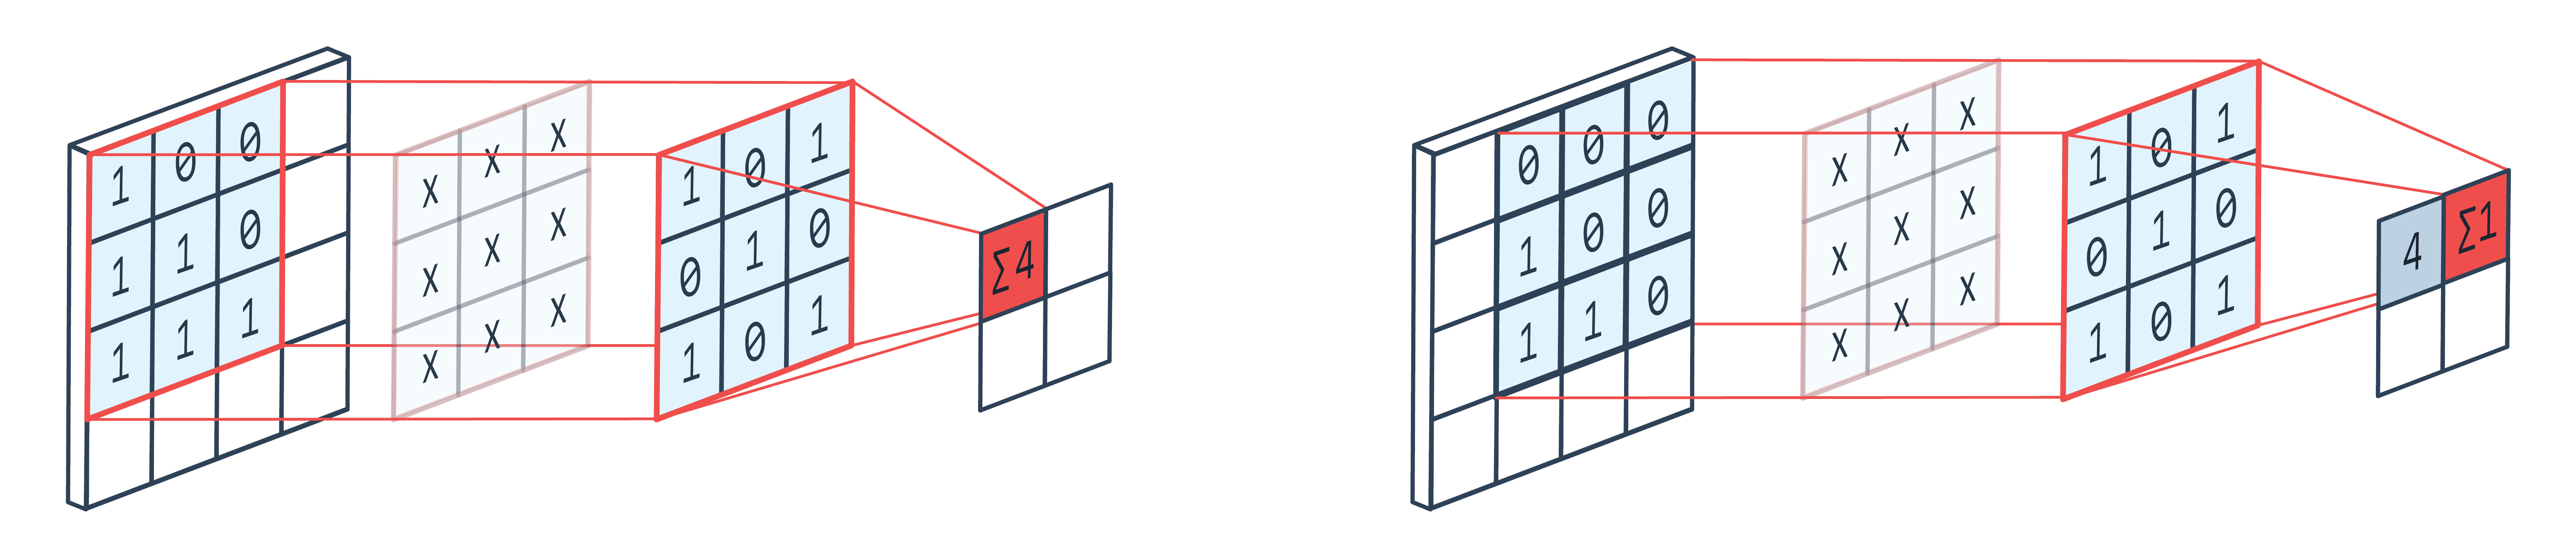
\includegraphics[width=.9\textwidth]{convolucion-2d}
  \caption{Ejemplo de aplicación de convolución 2D.}
  \label{fig:convolucion-2d}
\end{figure}

\begin{figure}[htpb]
  \centering
  %\hspace*{-2.5cm}
  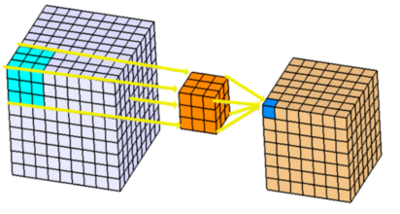
\includegraphics[width=.4\textwidth]{convolucion-3d}
  \caption{Ejemplo de aplicación de convolución 3D.}
  \label{fig:convolucion-3d}
\end{figure}

Notamos que si las imágenes son muy grandes al aplicar diversas capas de filtros el número de pesos puede elevarse bastante y hacerse computacionalmente inviable, por lo que se suele aplicar una técnica de discretización/reducción de dimensión llamada \emph{max-pooling} o \emph{average-pooling }\cite{graham2014fractional}. Esta técnica es igual que aplicar un filtro con $1$ solo que en vez de hacer la suma se toma o bien el máximo o la media de los valores, conseguiendo reducir la dimensión de la imagen tomando representantes de cada área a la que se le aplica; un ejemplo de esto está en \autoref{fig:pooling} \cite{yani2019application}.

\begin{figure}[htpb]
  \centering
  %\hspace*{-2.5cm}
  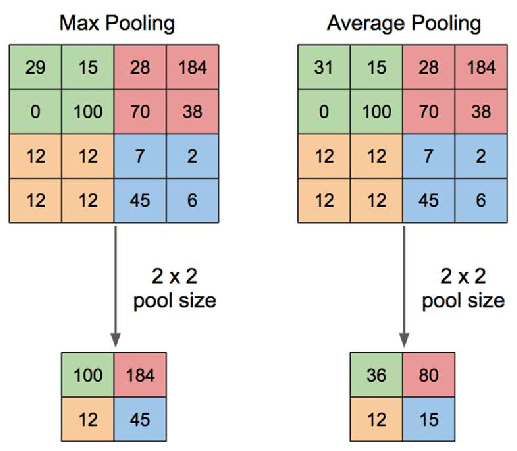
\includegraphics[width=.45\textwidth]{pooling}
  \caption{Ejemplo de \emph{max-pooling} y \emph{average-pooling}.}
  \label{fig:pooling}
\end{figure}

Generalmente la estructura de una CNN tiene dos partes: la primera parte se corresponde al \textbf{extractor de características} que obtiene estas características aplicando filtros mediante el uso de convoluciones con \emph{pooling}, y la segunda es el \textbf{clasificador} que es una red densa (como si fuese una \emph{feed-forward neural network}) que utiliza las características extraídas anteriormente para clasificar las imágenes.

Un ejemplo de esta estructura para clasificar imágenes de dígitos lo tenemos en \autoref{fig:ejemplo-cnn} \cite{saha2018cnn}.

\begin{figure}[htpb]
  \centering
  %\hspace*{-2.5cm}
  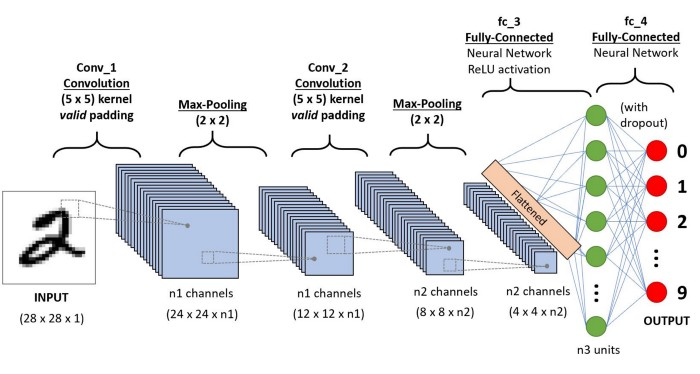
\includegraphics[width=.8\textwidth]{ejemplo-cnn}
  \caption{Ejemplo de estructura de CNN.}
  \label{fig:ejemplo-cnn}
\end{figure}

\subsection{Autocodificador}\label{sec:autoencoder}

Los \textbf{autocodificadores} (\emph{autoencoder, AE}) \cite{mcclelland1986parallel} son redes neuronales modeladas tipicamente para problemas de aprendizaje no supervisado que intentan replicar la entrada en la salida, intentando que en el proceso la red aprenda las características fundamentales de los datos consiguiendo así una \textbf{representación} comprimida de los datos (están codificados).

Veamos la estructura (\autoref{fig:ej-ae}, \cite{sancho2020ae}) que generalmente se divide en dos partes:

\begin{enumerate}
  \item \textbf{Codificador} (\emph{enconder}): la parte de la red que recibe la entrada y va disminuyendo el tamaño de las salidas hasta llegar al vector donde queda codificado la entrada.
  \item \textbf{Descodificador} (\emph{decoder}): la parte de la red que recibe el vector codificador y va aumentado su tamaño hasta llegar a la salida donde reconstruye la entrada original.
\end{enumerate}

\begin{figure}[htpb]
  \centering
  %\hspace*{-2.5cm}
  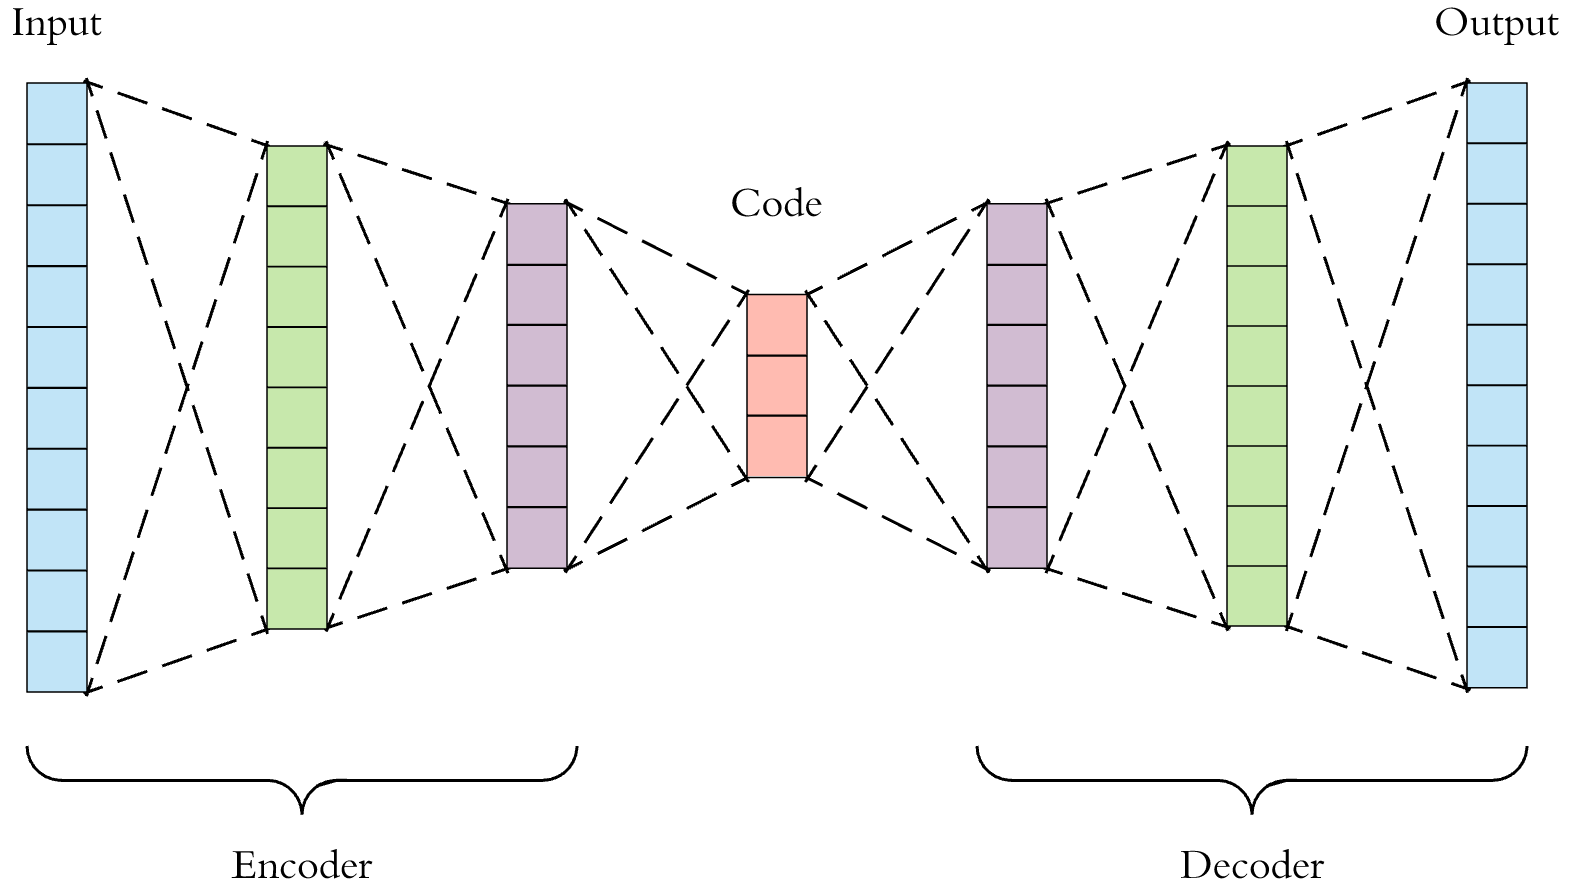
\includegraphics[width=.8\textwidth]{ae}
  \caption{Ejemplo de estructura de un autocodificador}
  \label{fig:ej-ae}
\end{figure}

Este tipo de redes son útiles cuando necesitamos aprender algún patrón o estructura de los datos, o cuando necesitamos comprimir en una dimensión reducida datos muy grandes.

También mencionamos los \textbf{autocodificadores variacionales} (\emph{variational autoencoders}, VAE) que lo que cambian respecto los autocodificadores es el tipo de codificación que se está haciendo, en vez de un vector cualquiera
se busca obtener una representación con \textbf{distribuciones de probabilidad gaussiana}, para ello se toman dos vectores uno de medias $\pmb{\mu} = (\mu_1, \ldots, \mu_n)^T$ y otro de varianzas $\pmb{\sigma}^2 = (\sigma_1^2, \ldots, \sigma_n^2)^T$ de manera que si los juntamos obtenemos un vector de variables aleatorias que siguen distribuciones gausisianas $\mathcal{N}(\pmb{\mu}, diag(\pmb{\sigma}^2))$ de las que podemos obtener una muestra que recontruimos en la salida \autoref{fig:ej-vae} \cite{sancho2020ae}.

\begin{figure}[htpb]
  \centering
  %\hspace*{-2.5cm}
  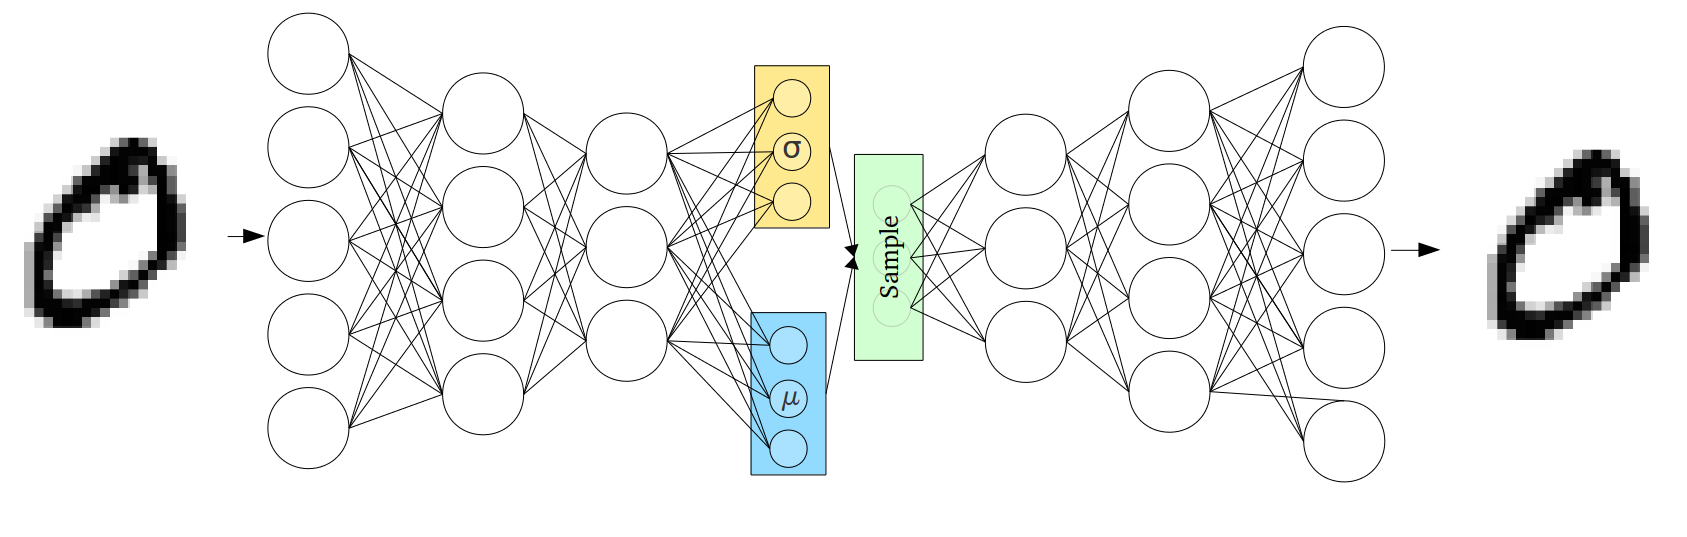
\includegraphics[width=1.\textwidth]{vae}
  \caption{Ejemplo de estructura de un autocodificador variacional}
  \label{fig:ej-vae}
\end{figure}

Para que el entrenamiento se haga correctamente se debe introducir un término nuevo a la función de pérdida que teníamos para la reconstrucción de la entrada: la \textbf{Divergencia de Kullback-Leiber} \cite{kullback1951information} que \emph{a grosso modo} mide la diferencia entre dos distribuciones de probabilidad. Para poder efectuar la diferencia necesitamos saber cual es la distribución latente, pero esta es desconocida así que imponemos la hipótesis de que sea una distribución normal $\mathcal{N}(\textbf{0}, \textbf{1})$ y ya podemos obtener la divergencia como
\begin{equation*}
  D_{KL}(\mathcal{N}(\pmb{\mu}, diag(\pmb{\sigma}^2)) || \mathcal{N}(\textbf{0}, \textbf{1})) = \dfrac{1}{2} \sum^{n}_{i = 1} \left(\sigma^2_i + \mu^2_i - 1 - \log(\sigma^2_i) \right).
  \label{eq:divergencia}
\end{equation*}

Gracias a este diseño, estos modelos son muy útiles para cuando se quieren generar nuevos datos sintéticos que sigan los mismos patrones de los datos donde fueron entrenados, haciendo que parezcan datos auténticos. Por ejemplo podríamos crear un generador de caras en \autoref{fig:caras} \cite{sancho2020ae}.

\begin{figure}[htpb]
  \centering
  %\hspace*{-2.5cm}
  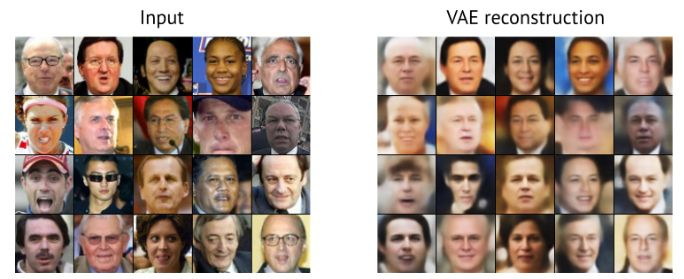
\includegraphics[width=.8\textwidth]{caras}
  \caption{Ejemplo de generador de caras usando un VAE entrenado con caras reales.}
  \label{fig:caras}
\end{figure}

\subsection{Redes Generativas Antagónicas}

Las \textbf{Redes Generativas Antagónicas} (\emph{Generative Adversarial Nets}, GAN) \cite{goodfellow2014generative} es uno de los tipos más novedosos de redes neuronales actualmente cuyo objetivo es crear muestras sintéticas nuevas a partir de una muestra real. Esta arquitectura está compuesta por dos redes distintas: la red \textbf{generadora} (\emph{generator}) y la red \textbf{discriminadora} (\emph{discriminator}). La generadora toma ruido aleatorio como entrada y trata de producir una salida que sea muy parecida a los datos reales, por otro lado la discriminadora toma la entrada del generador y una muestra real del \emph{dataset} y su objetivo es acertar cual es la verdadera (\autoref{fig:gan}, \cite{thalles2018gan}).

\begin{figure}[htpb]
  \centering
  %\hspace*{-2.5cm}
  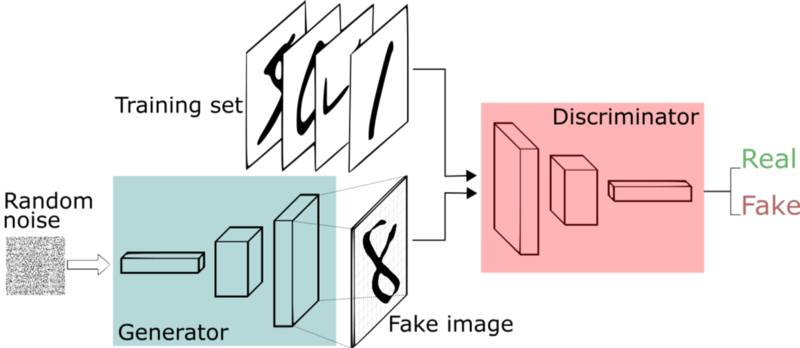
\includegraphics[width=.8\textwidth]{gan}
  \caption{Estructura de una red GAN con dígitos.}
  \label{fig:gan}
\end{figure}

Podemos entender este tipo de red parecido a un juego de suma cero ya que la función de pérdida que intenta minimizar uno es la contraria al otro, por lo que se tiene una especie de \emph{lucha} en el entrenamiento. El generador empieza mejorando los datos fabricados lo que provoca que el discriminador le cueste más diferenciar y se entrene para mejorar su capacidad de discriminación que hace que el generador tenga que hacer mejores fabricaciones; y así cíclicamente, dándonos al final de entrenamiento un generador que devuelve muestras casi imposibles de diferenciar de una real.

Como ya ocurría con los VAE estos modelos son muy útiles para crear datos nuevos que sean prácticamente reales o también para la creación de videos y fotos falsas, modificando las caras de las personas por otras (las famosas \emph{Deepfake} \cite{nguyen2020deepfake}).

\subsection{Redes Neuronales Recurrentes}

Finalmente vemos el tipo de arquitectura en el que nos centraremos, las \textbf{Redes Neuronales Recurrentes} (\emph{Recurrent Neural Networks}, RNN) \cite{elman1990finding} tratan de aprovechar la dependencia temporal que presentan ciertos tipos de datos (frases, música, series temporales...) mediante un flujo de información de entradas anteriores hacia las posteriores (\autoref{fig:rnn-rolled} \cite{christopher2015lstm}).

\begin{figure}[htpb]
  \centering
  %\hspace*{-2.5cm}
  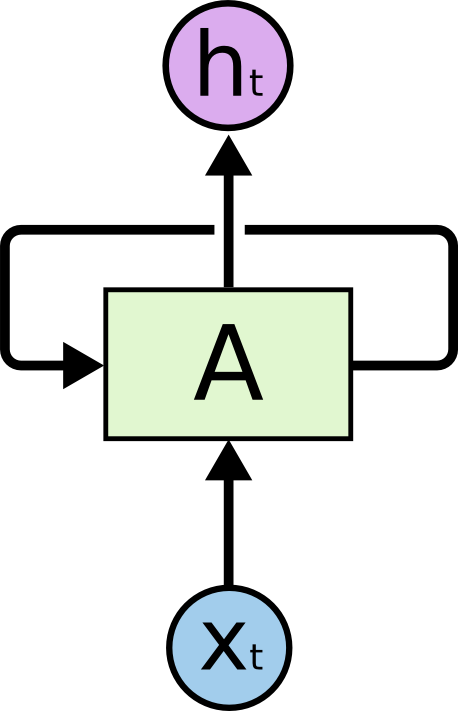
\includegraphics[width=.15\textwidth]{rnn-rolled}
  \caption{Estructura de una RNN.}
  \label{fig:rnn-rolled}
\end{figure}

Esta estructura nos viene a decir que para una cierta entrada $x_t$ el modelo $A$ nos proporciona una salida $h_t$ pero además se pasa a si mismo, retroalimentándose, una información obtenida en función de $x_t$ que se tendrá en cuenta para entradas posteriores ($x_{t + 1}$, $x_{t + 2}$...). Aunque en principio pueda parecer una estructura complicada se puede \emph{desenrollar} en función del tiempo, quedándonos una estructura muy simple (\autoref{fig:rnn-unrolled}, \cite{christopher2015lstm}).

\begin{figure}[htpb]
  \centering
  %\hspace*{-2.5cm}
  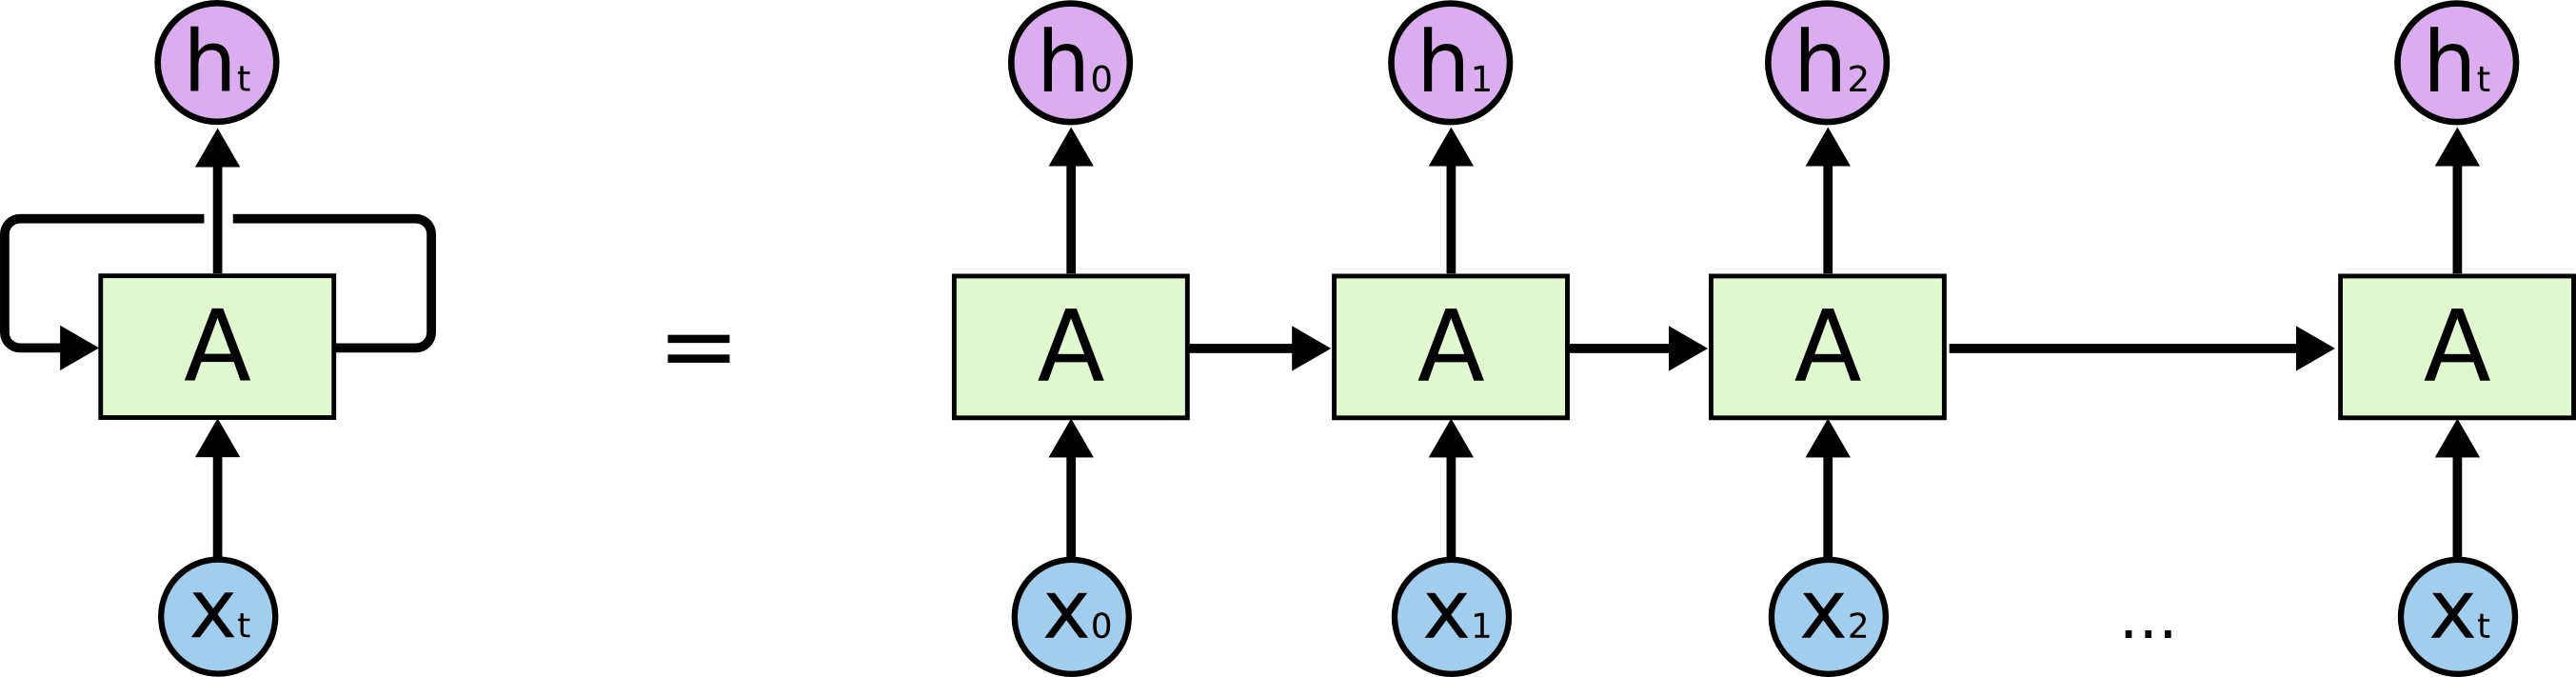
\includegraphics[width=.8\textwidth]{rnn-unrolled}
  \caption{Estructura de una RNN desenrollada.}
  \label{fig:rnn-unrolled}
\end{figure}

Queda claro así cómo según bajo ciertas entradas anteriores, que es lo que proporciona el \textbf{contexto}, la salida de una entrada posterior puede variar enormemente. Así, en las RNN se diseña una neurona especial para enviar la información de manera relativamente sencilla: se une la entrada $x_t$ con la salida de la entrada anterior $h_{t-1}$, que llamaremos \textbf{estado oculto}, a una neurona normal como las conocemos (\autoref{fig:rnn-cells}, \cite{christopher2015lstm}). Tomando como función de activación $\tanh$, La fórmula de cada neurona quedará terminada por los pesos $W$, dada por
\begin{equation*}
  h_t = \tanh \left(W^T \begin{bmatrix} h_{t-1} & x_t & 1 \end{bmatrix}^T\right).
  \label{eq:rnn}
\end{equation*}

\begin{figure}[htpb]
  \centering
  %\hspace*{-2.5cm}
  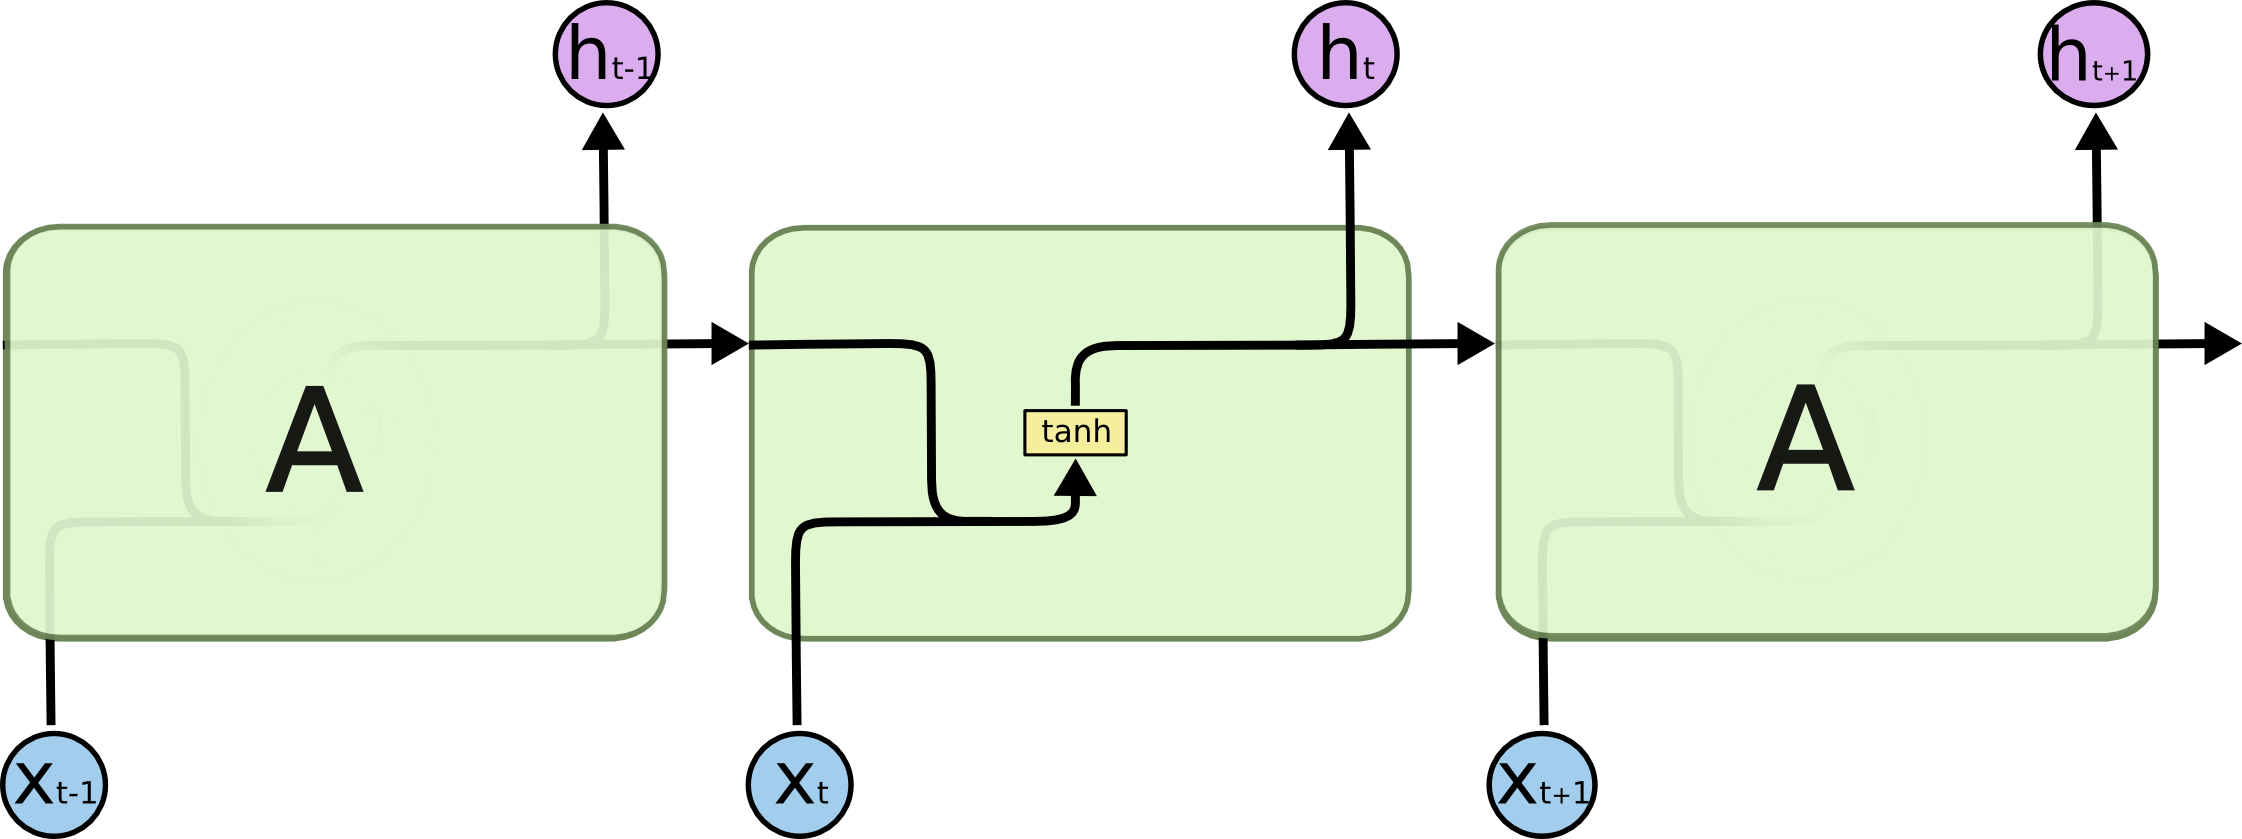
\includegraphics[width=.9\textwidth]{rnn-cells}
  \caption{Estructura de una neurona en una RNN.}
  \label{fig:rnn-cells}
\end{figure}

Sin embargo hay un gran problema: cierta información útil para una entrada \textbf{muy posterior} en el tiempo probablemente no llegue debido a que hay un salto temporal muy grande entre las entradas (\autoref{fig:rnn-longterm}, \cite{christopher2015lstm}), es decir, el modelo no capta bien las \textbf{dependencias temporales a largo plazo} (\emph{long-term dependecies}) \cite{bengio1994learning}.

\begin{figure}[htpb]
  \centering
  %\hspace*{-2.5cm}
  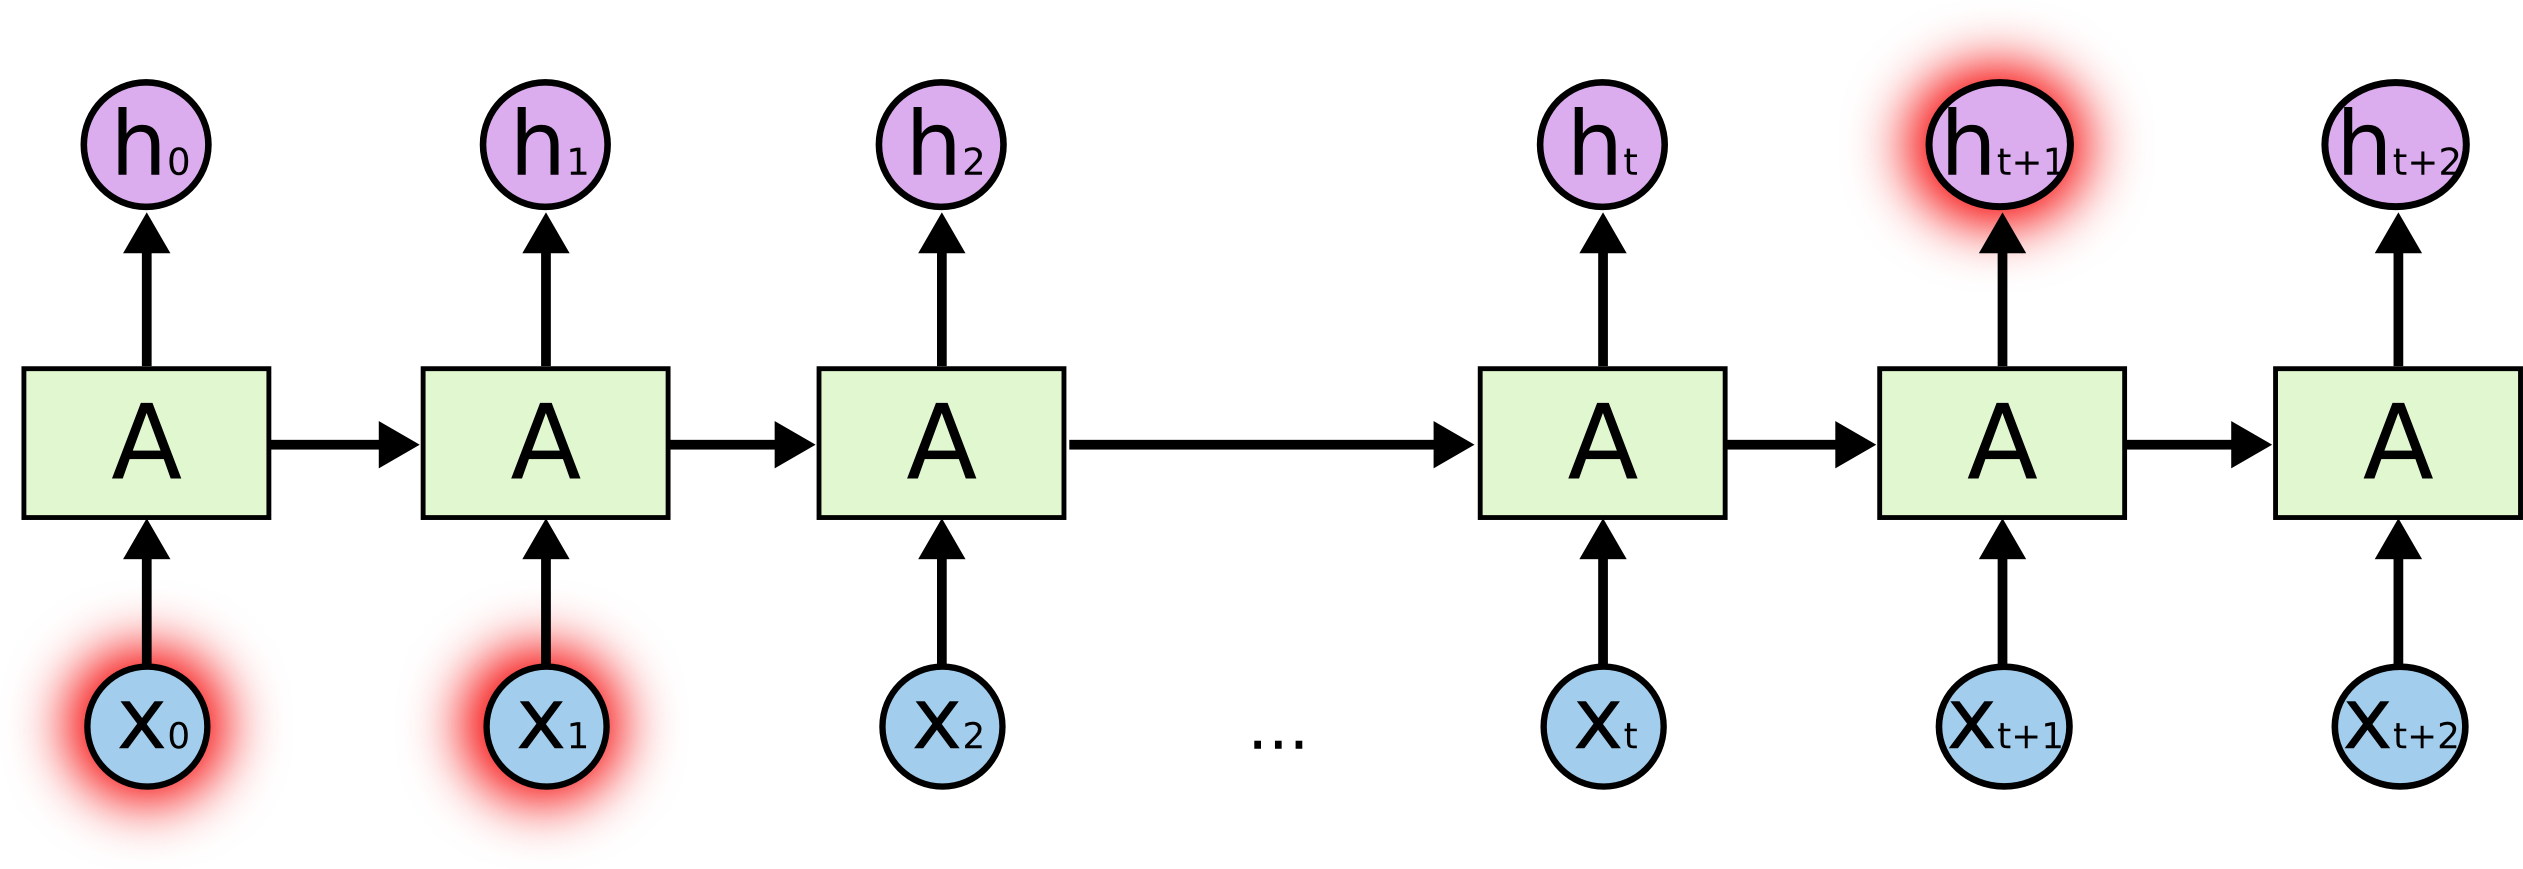
\includegraphics[width=.9\textwidth]{rnn-longterm}
  \caption{La información de $x_1$ y $x_2$ no llega para $h_{t+1}$.}
  \label{fig:rnn-longterm}
\end{figure}

Este obstáculo es consecuencia directa del \textbf{problema del desvanecimiento del gradiente} (\emph{vanishing gradient problem}) que ocurre al entrenar redes neuronales muy profundas, ya que, recordando que para obtener el gradiente íbamos propagando el error desde la última capa hasta la primera capa, el gradiente va disminuyendo poco a poco y si la red es muy extensa entonces va disminuyendo a cero provocando que las capas dejen de actualizarse. Lo que viene a decirnos resumidamente es que la información se pierde rápidamente en el tiempo, por lo que no podemos dar información de entradas muy separadas. También es posible que pase el caso contrario, que el gradiente \textbf{explote} (\emph{explodes}) (aumente hasta valores que sobrepasan el límite de representación de la máquina); en cualquier caso las RNN suelen ser modelos inestables debido a esto \cite{Goodfellow-et-al-2016}.

Para resolver este problema surgen las redes \emph{Long Short Term Memory} (LSTM) \cite{hochreiter1997long}, que consiguen aprender la información tanto a corto como a largo plazo. Estas redes serán las que dedicaremos más atención, y sobre las que nos basaremos para construir nuestros modelos de aprendizaje profundo en el desarrollo del trabajo.

\section{LSTM}

\subsection{Estructura general}

La idea que añade una neurona LSTM para solucionar las dependencias temporales a largo plazo es permitir el paso de la información, recordando u olvidándola, mediante \textbf{puertas} (\emph{gates}) y añadiendo otro flujo de información además del estado oculto $h_t$: el estado celular $C_t$. Este estado intenta emular una especie de \emph{memoria} que irá llevando información relevante desde el principio de la secuencia de entradas hasta mucho más adelante, evitando la pérdida a largo plazo de las RNN.

Primero veamos como está constituida una puerta (\autoref{fig:gate}, \cite{christopher2015lstm}): una neurona normal que recibe una entrada y con función de activación \textbf{sigmoide}, cuya salida realiza una operación de multiplicación coordenada a coordenada con la información que se está regulando. Como la función sigmoide devuelve valores entre $[0, 1]$, al multiplicarlos por la información nos permite, o bien olvidar cuando los valores sean cercanos a 0 ó recordarlos si son cercanos a 1.

\begin{figure}[htpb]
  \centering
  %\hspace*{-2.5cm}
  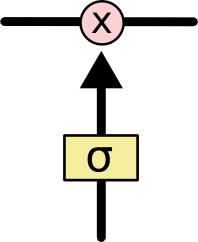
\includegraphics[width=.2\textwidth]{gate}
  \caption{Ejemplo de puerta.}
  \label{fig:gate}
\end{figure}

Fijémonos ahora en la estructura general de una neurona o célula LSTM (\autoref{fig:lstm-cells}, \cite{christopher2015lstm}) y vayamos paso por paso para entender todas los operaciones que tienen lugar. Apreciamos cómo el estado celular viene dado por el flujo superior de la célula, mientras que el estado oculto entra y sale por el inferior y consideramos además que $\sigma \equiv sigmoide$.

\begin{figure}[htpb]
  \centering
  %\hspace*{-2.5cm}
  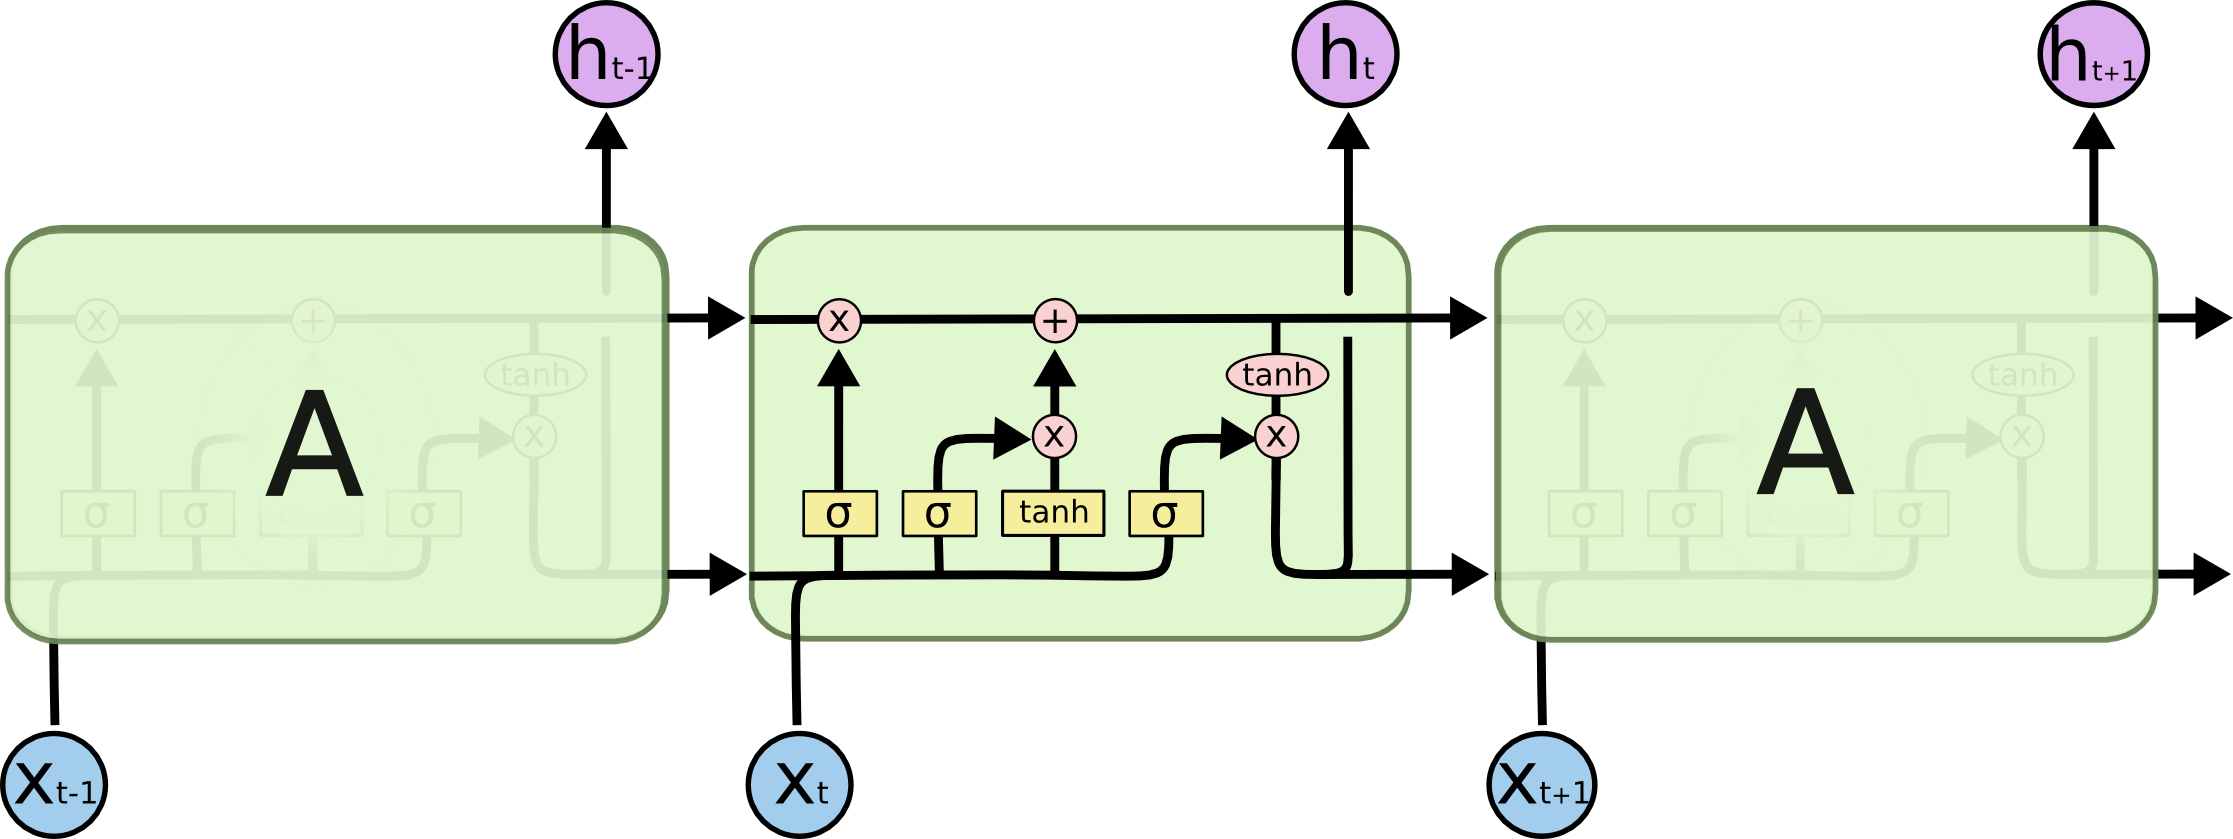
\includegraphics[width=1.\textwidth]{lstm-cells}
  \caption{Esquema de célula LSTM.}
  \label{fig:lstm-cells}
\end{figure}

Primero nos encontramos con la \textbf{puerta del olvido} (\emph{forget gate}), la puerta que se encarga de decidir si la información del estado celular anterior $c_{t-1}$ debería olvidarse o no en base a el estado oculto anterior $h_{t-1}$ y la entrada actual $x_t$; de esta manera controlamos qué información de las variables anteriores recordamos (\autoref{fig:forget} \cite{christopher2015lstm}). El valor de la puerta $f_t$ queda determinado por los pesos $W_f$, en base a
\begin{equation*}
  f_t = \sigma\left(W_f^T \begin{bmatrix} h_{t-1} & x_t & 1 \end{bmatrix}^T \right).
  \label{eq:forget}
\end{equation*}

\begin{figure}[htpb]
  \centering
  %\hspace*{-2.5cm}
  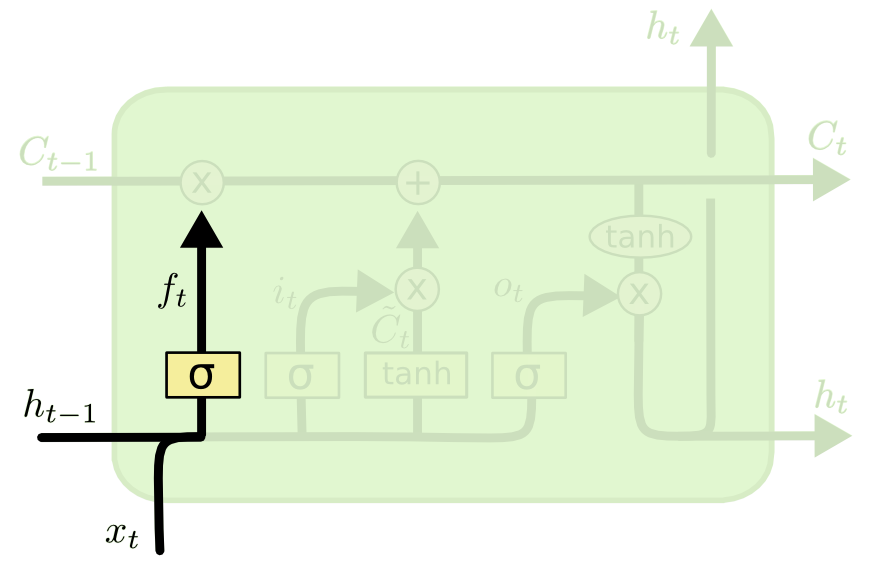
\includegraphics[width=.5\textwidth]{forget}
  \caption{Puerta del olvido $f_t$.}
  \label{fig:forget}
\end{figure}

A continuación tenemos la \textbf{puerta de entrada} (\emph{input gate}) que es la que determina si la nueva información en base a la entrada actual $x_t$ y el estado oculto anterior $h_{t-1}$, se debe incluir o no en el estado celular; indicándonos si esta entrada es relevante o no (\autoref{fig:input} \cite{christopher2015lstm}). Tenemos por un lado el valor de la puerta $i_t$ y el valor de la neurona que tiene la información $\widetilde{C}_t$ donde ambas quedan determinadas por sus pesos $W_i$, $W_{\widetilde{C}}$ con las respectivas fórmulas dadas por
\begin{equation*}
  i_t = \sigma\left(W_i^T \begin{bmatrix} h_{t-1} & x_t & 1 \end{bmatrix}^T\right),
  \label{eq:input1}
\end{equation*}
y
\begin{equation*}
  \widetilde{C}_t = \tanh\left(W_{\widetilde{C}}^T \begin{bmatrix} h_{t-1} & x_t & 1 \end{bmatrix}^T\right).
  \label{eq:input2}
\end{equation*}

\begin{figure}[htpb]
  \centering
  %\hspace*{-2.5cm}
  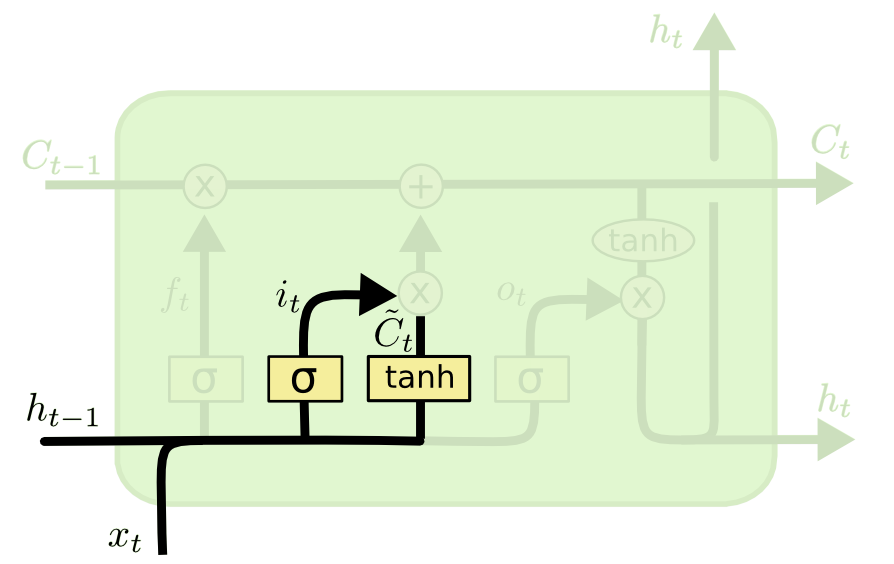
\includegraphics[width=.5\textwidth]{input}
  \caption{Puerta de entrada $i_t$ e información de la neurona $\widetilde{C}_t$.}
  \label{fig:input}
\end{figure}

Llegamos al \textbf{estado celular} que es el valor que lleva la información importante a lo largo de la secuencia y que queda determinada por su entrada anterior $C_{t-1}$ junto a la puerta del olvido $f_t$ y la información actual $\widetilde{C}_t$ junto a la puerta de entrada $i_t$ (\autoref{fig:celular} \cite{christopher2015lstm}). Su valor $C_t$ queda determinada por los valores anteriores en base a la expresión siguiente
\begin{equation*}
  C_t = f_t C_{t-1} + i_t \widetilde{C}_t.
  \label{eq:celular}
\end{equation*}

\begin{figure}[htpb]
  \centering
  %\hspace*{-2.5cm}
  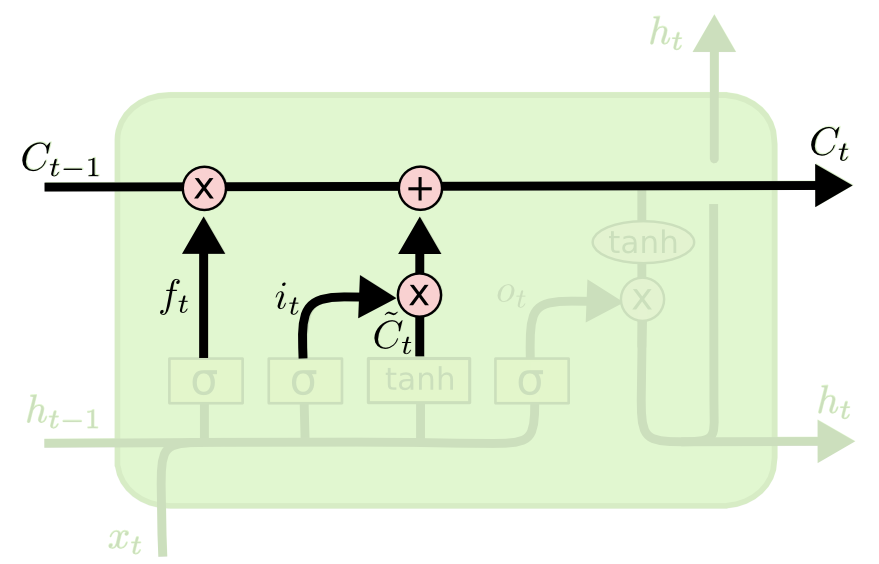
\includegraphics[width=.5\textwidth]{celular}
  \caption{Estado celular $C_t$.}
  \label{fig:celular}
\end{figure}

Finalmente acabamos con la \textbf{puerta de salida} (\emph{output gate}) que regula la información del estado celular $C_t$ que devuelve como salida la célula, es decir, el estado oculto $h_t$ (\autoref{fig:output} \cite{christopher2015lstm}). Tenemos el valor de la puerta $o_t$, determinado por la última matriz de pesos $W_o$, y el estado celular $h_t$ calculados con las respectivas expresiones
\begin{equation*}
  o_t = \sigma\left(W_o^T \begin{bmatrix} h_{t-1} & x_t & 1 \end{bmatrix}^T\right),
  \label{eq:output1}
\end{equation*}
y
\begin{equation*}
  h_t = o_t \tanh\left(C_t\right).
  \label{eq:output2}
\end{equation*}

\begin{figure}[htpb]
  \centering
  %\hspace*{-2.5cm}
  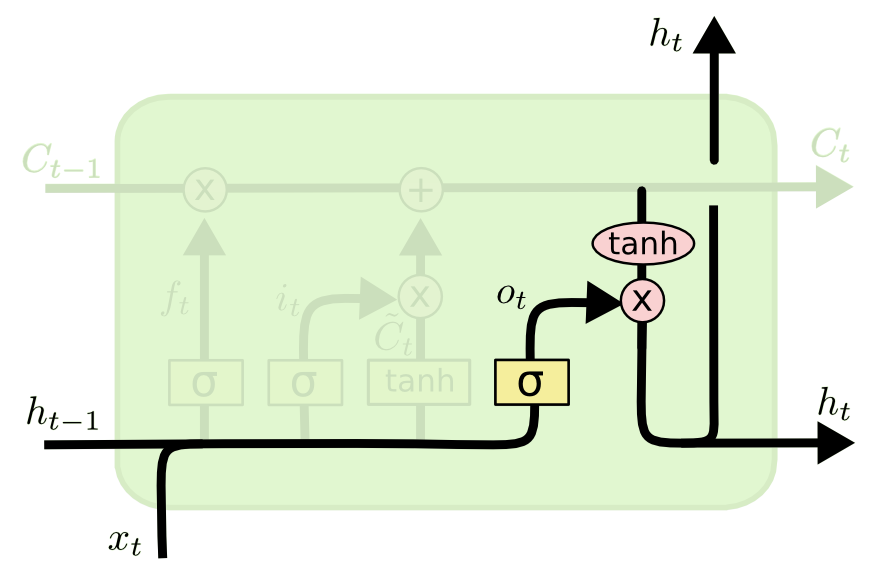
\includegraphics[width=.5\textwidth]{output}
  \caption{Puerta de salida $o_t$.}
  \label{fig:output}
\end{figure}

Observamos que cada célula LSTM tiene 4 neuronas normales con sus pesos respectivos que aprender, siendo de estas 3 para puertas (olvido, entrada y salida) y la cuarta para la información de la propia célula. Este tipo de neurona es mucho más compleja y con muchos mas parámetros libres que aprender que la versión que habíamos considerado en las RNN pero permite flujos de información mucho más ricos al permitir olvidar o memorizar a voluntad y por supuesto que se pueda transmitir información importante desde tiempos muy separados.

\subsection{Variantes}

De esta célula se han creado muchas variantes que generalmente suelen ser modificaciones pequeñas que son ciertamente interesantes. Por ejemplo, \cite{gers2000recurrent} añade conexiones del estado celular anterior $C_{t-1}$ hacia las puertas de manera que los valores quedan actualizados así
\begin{gather*}
  f_t = \sigma\left(W_f^T \begin{bmatrix} C_{t-1} & h_{t-1} & x_t & 1 \end{bmatrix}^T \right), \\
  i_t = \sigma\left(W_i^T \begin{bmatrix} C_{t-1} & h_{t-1} & x_t & 1 \end{bmatrix}^T\right), \\
  o_t = \sigma\left(W_o^T \begin{bmatrix} C_{t-1} & h_{t-1} & x_t & 1 \end{bmatrix}^T\right).
  \label{eq:variante1}
\end{gather*}
obteniendo esta estructura (\autoref{fig:variante1} \cite{christopher2015lstm}).

\begin{figure}[htpb]
  \centering
  %\hspace*{-2.5cm}
  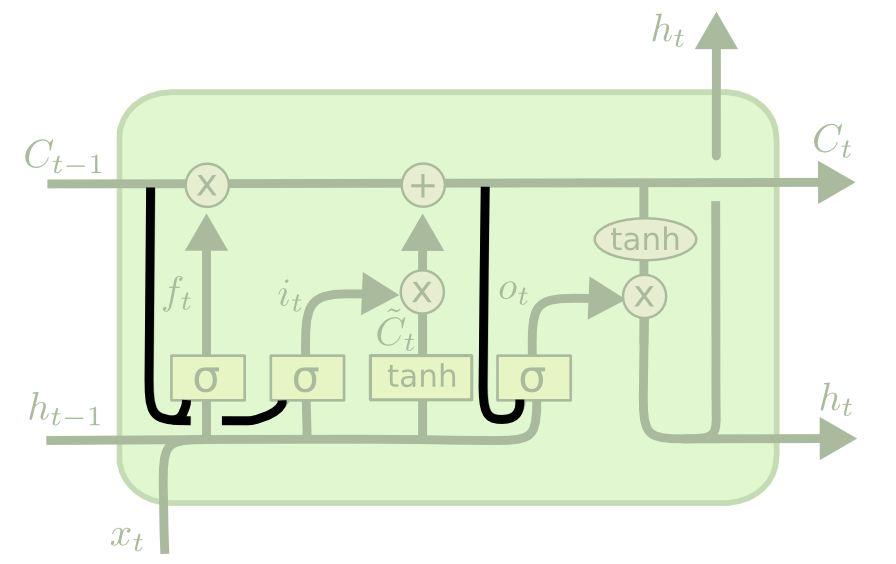
\includegraphics[width=.5\textwidth]{variante1}
  \caption{Variante que introduce cauces de $C_{t-1}$ con las puertas.}
  \label{fig:variante1}
\end{figure}

Otra modificación de \cite{gers2000recurrent} considera unificar las puertas de olvido $f_t$ y entrada $i_t$ de manera que si una puerta considera olvidar la información la otra puerta recuerda; de esta manera solo recordamos algo nuevo si olvidamos lo pasado, y solo recordamos lo pasado si olvidamos lo nuevo (\autoref{fig:variante2} \cite{christopher2015lstm}). Las fórmulas de $C_t$ y $i_t$ actualizadas quedan como
\begin{gather*}
  i_t = 1 - f_t, \\
  C_t = f_t C_{t-1} + (1 - f_t) \widetilde{C}_t.
  \label{eq:variante2}
\end{gather*}

\begin{figure}[htpb]
  \centering
  %\hspace*{-2.5cm}
  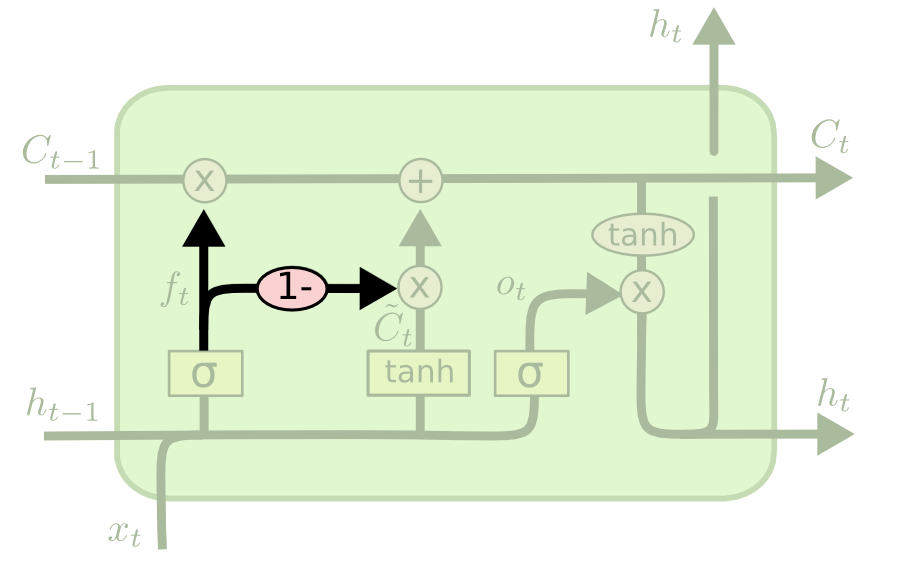
\includegraphics[width=.5\textwidth]{variante2}
  \caption{Variante que sustituye la puerta de entrada por la negación de la del olvido.}
  \label{fig:variante2}
\end{figure}

Finalmente nombramos una de las variantes más conocidas, la \textbf{Unidad Recurrente con Puertas} (\emph{Gated Recurrent Unit}, GRU) \cite{cho2014learning} que intenta simplificar la célula LSTM para reducir los cálculos y conseguir un entrenamiento mucho más rápido mediante la fusión el estado celular con el oculto, así como también las puertas del olvido y de entrada (formando la puerta de actualización $z_t$), quitando la puerta de salida y añadiendo una nueva llamada de reinicio $r_t$. Ahora la célula solo devuelve el estado oculto $h_t$ en función de la siguientes fórmulas
\begin{gather*}
  z_t = \sigma\left(W_z^T \begin{bmatrix} h_{t-1} & x_t \end{bmatrix}^T\right), \\
  r_t = \sigma\left(W_r^T \begin{bmatrix} h_{t-1} & x_t \end{bmatrix}^T \right), \\
  \widetilde{h}_t = \tanh\left(W_{\widetilde{h}}^T \begin{bmatrix} r_t h_{t-1} & x_t \end{bmatrix}^T\right), \\
  h_t = (1 - z_t)h_{t-1} + z_t \widetilde{h}_t.
  \label{eq:gru}
\end{gather*}
junto a la nueva estructura (\autoref{fig:gru}, \cite{christopher2015lstm}).

\begin{figure}[htpb]
  \centering
  %\hspace*{-2.5cm}
  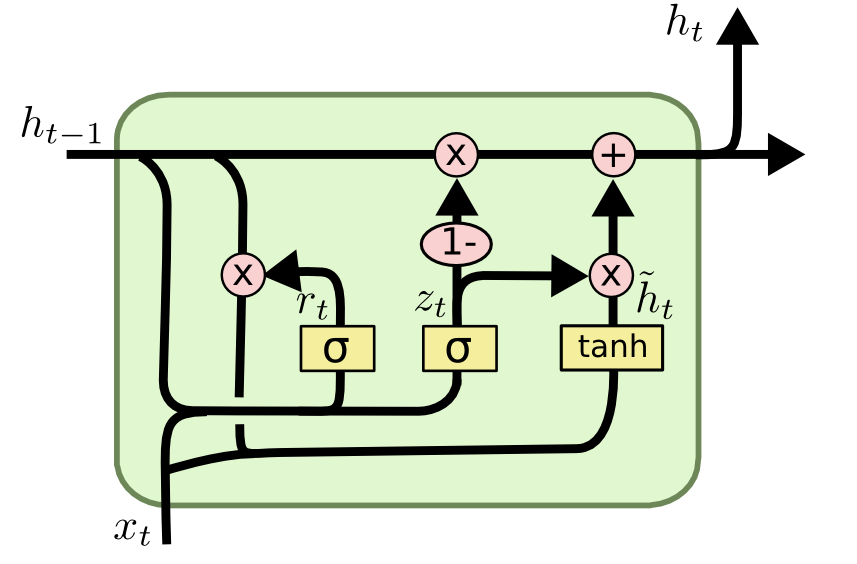
\includegraphics[width=.5\textwidth]{gru}
  \caption{Estructura de la variante GRU.}
  \label{fig:gru}
\end{figure}

Sin embargo, en \cite{greff2016lstm} se hace una comparación de rendimiento entre todas variantes y se observó que no había un modelo que fuese especialmente mejor, todas se comportaban más o menos igual de bien, si bien \cite{gers1999learning} observaron que la versión de LSTM añadiendo un término de error de 1 en la puerta del olvido la hacía la versión más potente de todas las consideradas \cite{Goodfellow-et-al-2016}. Bajo estas razones tomaremos en nuestros modelos las versiones LSTM normales.

\subsection{Recorte}

A pesar de que la arquitectura LSTM evita enormemente el problema del desvanecimiento del gradiente, es posible encontrar en algún caso de entrenamiento que el gradiente explote (la norma del gradiente diverge). Si ocurre esto una técnica muy interesante de utilizar es el método del \textbf{recorte de gradiente} (\emph{clipping gradient}) \cite{pascanu2013difficulty}, que se encarga de ponerle un \emph{tope} a la norma del gradiente cuando supera cierto valor.

Cada vez que se obtiene el gradiente $\textbf{g}$ se aplica la siguiente regla
\begin{equation*}
  \textbf{g}' = \begin{cases} \textbf{g} & \text{si } ||\textbf{g}|| \leq v, \\ v\dfrac{\textbf{g}}{||\textbf{g}||} & \text{en caso contrario,} \end{cases}
  \label{eq:clipping}
\end{equation*}
antes de actualizar los pesos, evitando así que la red use valores enormes del gradiente para actualizar los pesos, haciendo que la red se inestabilice y ya no sirva \cite{Goodfellow-et-al-2016}.

\endinput


% --------------------------------------------------------------------
% APPENDIX: Opcional
% --------------------------------------------------------------------

\appendix % Reinicia la numeración de los capítulos y usa letras para numerarlos
\pdfbookmark[-1]{Apéndices}{appendix} % Alternativamente podemos agrupar los apéndices con un nuevo \part{Apéndices}

%% !TeX root = ../libro.tex
% !TeX encoding = utf8

\chapter{Documentación}\label{ap:documentacion}

En este apéndice se deja la documentación en estilo \emph{python} de la documentación de las distintas clases, métodos y funciones más importantes implementados en el proyecto.

\section{Selección de Modelos}

Las clases implementadas para la parte de selección de modelos que se pueden encontrar en la carpeta $PV/src$.

\subsection{Perturbated Validation}

Esta clase y sus métodos se encuentran en el archivo $PV.py$.

\paragraph{PV}

Clase PV que implementa el método para calcular y manejar la heurística PV. Guarda los datos de las series originales, las perturbaciones realizadas, los ratio de error, el nombre del dataset que se está perturbando, y valores auxiliares para imprimir gráficas del cálculo del PV.

\begin{lstlisting}
class PV:
    """
        Clase que implementa Perturbation Validation (PV).

        Attributes
        ----------
        X : np.array
            Dataset
        y : np.array
            Conjuto de etiquetas perturbadas
        ds_name : str
            Nombre del dataset
        errs : np.array
            Errores tomados
        counter : int
            Contador auxiliar
        fig : Figure
            Figura actual
        ax : Axes
            Ejes actuales
    """
\end{lstlisting}

\paragraph{Constructor}

Constructor de la clase PV que necesita los datos originales, el número de perturbaciones, el nombre del \emph{dataset}, y el inicio y fin de los ratio de error. Crea los conjuntos de etiquetas perturbadas.

\begin{lstlisting}
def __init__(self, X, y, n_pv = 5, ds_name = "", err_ini = 0.1,
                 err_fin = 0.3):
        """
            Inicializa la clase creando las etiquetas perturbadas.

            Las perturbaciones se realizan tomando un %err de cada
            clase, poniendole otra etiqueta distinta.

            Se toman "n_pv" puntos entre [err_ini, err_fin].

            Parameters
            ----------
            X : np.array
                Dataset
            y : np.array
                Etiquetas
            n_pv: int
                Número de puntos/errores
            ds_name: str
                Nombre del datases
            err_ini : float
                Error inicial
            err_fin : float
                Error final
        """
\end{lstlisting}

\paragraph{Cálculo PV}

Método para calcular el valor PV de un modelo dado.

\begin{lstlisting}
def get_pv(self, clf, clf_name = "", plot = True):
        """
            Calcula el PV score para el clasificador.

            Parameters
            ----------
            clf : Classifier
                Clasificador
            clf_name : str
                Nombre del clasificador

            Returns
            -------
            pv : float
                PV score
            accs : list(float)
                accs obtenidos
        """
\end{lstlisting}

\paragraph{Dibujar cálculo PV}

Método para representar en una gráfica los valores de la métrica $acc$ obtenidos en el cálculo de PV junto a la recta de regresión obtenida.

\begin{lstlisting}
def plot_pv(self, errs, accs, poly, pv, clf_name = ""):
        """
            Dibuja los puntos y la recta de regresión en la figura actual.

            Parameters
            ----------
            errs : np.array
                Errores
            accs : np.array
                acc obtenidos
            poly : np.array
                Recta de regresión
            pv : float
                Valor PV
            clf_name : str
                Nombre del clasificador
        """
\end{lstlisting}

\paragraph{Guardar gráfica}

Método para guardar en una imagen .png el gráfico del método $plot\_pv$.

\begin{lstlisting}
def save_graph(self, name_fig):
        """
            Guarda el gráfico de los resultados en un .png

            Parameters
            ----------
            name_fig : str
                Nombre (ruta) de la imagen a guardar.
        """
\end{lstlisting}

\subsection{Clasificador LSTM}

Esta clase y sus métodos se encuentran en el archivo $LSTM.py$.

\paragraph{LSTM}

La clase LSTM que implementa el clasificador LSTM. Guarda el modelo LSTM, el número de clases, la longitud de las series, opciones de entrenamiento y para gráficas de entrenamiento.

\begin{lstlisting}
class LSTM(BaseEstimator):
    """
        Implementación de una red neuronal con capas LSTM.

        Attributes
        ----------
        counter : int, static
            Valor auxiliar para ruta de imagen
        model : Sequential
            Modelo red neuronal
        history : list
            Historial del entrenamiento
        n_clases : int
            Número de clases de las etiquetas
        input_shape : tuple
            Forma de los datos
        epochs: int
            Número de épocas para entrenamiento
        verbose : int
            Información sobre el entrenamiento
        save_hist : boolean
            Si guardar las gráficas de los entrenamientos
    """
\end{lstlisting}

\paragraph{Constructor}

Constructor de la clase LSTM que guarda opciones de entrenamiento.

\begin{lstlisting}
def __init__(self, epochs, n_neurs = 80, verbose = 0, save_hist = False,
             n_clases = -1):
        """
            Inicializamos la red LSTM.

            Attributes
            ----------
            epochs : int
                Número de épocas para entrenamiento
            n_neurs : int
                Número de neuronas LSTM
            verbose : int
                Información sobre el entrenamiento
            save_hist : boolean
                Si guardar las gráficas de los entrenamientos
            n_clases : int
                Número de clases a predecir
        """
\end{lstlisting}

\paragraph{Creación del modelo}

Método para crear el modelo LSTM.

\begin{lstlisting}
def create_model(self):
        """
            Crea el modelo LSTM.
        """
\end{lstlisting}

\paragraph{Compilar el modelo}

Compila el modelo con el optimizador ADAM y la función de pérdida entropía cruzada categórica.

\begin{lstlisting}
def compile_model(self):
        """
            Compila el modelo con optimizador ADAM y función de pérdida
            categorical_crossentropy.
        """
\end{lstlisting}

\paragraph{Entrenamiento}

Método para entrenar el modelo con el conjunto de datos, con las épocas guardadas, validación al 10\% y con parada temprana.

\begin{lstlisting}
def fit(self, X, y):
        """
            Entrenamos el modelo.

            Parameters
            ----------
            X : numpy.array
                Datos de entrenamiento
            y : numpy.array
                Etiquetas de entrenamiento
        """
\end{lstlisting}

\paragraph{Cálculo métrica}

Método para calcular la métrica $acc$ en el conjunto de datos pasado.

\begin{lstlisting}
def score(self, X, y):
        """
            Calcula el acc con los datos que se le pasan.

            Parameters
            ----------
            X : numpy.array
                Datos test
            y : numpy.array
                Etiquetas test

            Returns
            ----------
            acc : float
                accuracy obtenida
        """
\end{lstlisting}

\paragraph{Guardar gráfica de entrenamiento}

Método para guardar el historial de entrenamiento en una imagen.

\begin{lstlisting}
def save_history(self):
        """
            Guarda el historial en una imagen.
        """
\end{lstlisting}

\subsection{Clasificadores}

Los clasificadores adicionales que usamos para comparar modelos, comparten dos métodos generales: entrenamiento y cálculo de la métrica.

\paragraph{Entrenamiento}

Método que se encarga de entrenar el modelo usando una muestra de datos.

\begin{lstlisting}
def fit(self, X, y):
    """
        Entrena el modelo.

        Parameters
        ----------
        X : numpy.array
            Datos de entrenamiento
        y : numpy.array
            Etiquetas de entrenamiento
    """
\end{lstlisting}

\subparagraph{Cálculo de métrica}

Método que se encarga de calcular la métrica ($accuracy$) de un modelo en un conjunto de datos.

\begin{lstlisting}
def score(self, X, y):
    """
        Calcula el acc con los datos que se le pasan.

        Parameters
        ----------
        X : numpy.array
            Datos test
        y : numpy.array
            Etiquetas test

        Returns
        ----------
        acc : float
            accuracy obtenida
    """
\end{lstlisting}

\subsubsection{C4.5}

Esta clase y sus métodos se encuentran en el archivo $RClassifiers.py$.

\paragraph{C45}

La clase C45 que usa el árbol de decisión C4.5 que guarda el modelo.

\begin{lstlisting}
class C45(BaseEstimator):
    """
        Implementa el árbol de decisión C4.5.

        Attributes
        ----------
        model : clasificador en R
            El clasificador (clase en R)
    """
\end{lstlisting}

\subsubsection{C5.0}

Esta clase y sus métodos se encuentran en el archivo $RClassifiers.py$.

\paragraph{C50}

La clase C50 que usa el árbol de decisión C5.0 que guarda el modelo, y también el valor del \emph{boosting}.

\begin{lstlisting}
class C50(BaseEstimator):
    """
        Implementa el árbol de decisión C5.0 (con boosting o no).

        Attributes
        ----------
        model : clasificador en R
            El clasificador (clase en R)
        boosting : int
            El valor del boosting
    """
\end{lstlisting}

\paragraph{Constructor}

Constructor de la clase C50 que se le pasa el número de \emph{boosting} que se necesite.

\begin{lstlisting}
def __init__(self, boosting = 10):
        """
            Inicializa el clasificador.

            Parameters
            ----------
            boosting : int
                El valor del boosting
        """
\end{lstlisting}

\subsubsection{Recursive Partioning Tree}

Esta clase y sus métodos se encuentran en el archivo $RClassifiers.py$.

\paragraph{RPart}

Clase que usa el árbol RPart.

\begin{lstlisting}
class RPart(BaseEstimator):
    """
        Implementa el árbol de decisión RPart (Recursive Partioning Tree).

        Attributes
        ----------
        model : clasificador en R
            El clasificador (clase en R)
    """
\end{lstlisting}

\subsubsection{Condicional Tree}

Esta clase y sus métodos se encuentran en el archivo $RClassifiers.py$.

\paragraph{CTree}

La clase CTree implementa el uso del árbol de decisión Condicional Tree.

\begin{lstlisting}
class CTree(BaseEstimator):
    """
        Implementa el árbol de decisión CTree (Conditional Inference Tree).

        Attributes
        ----------
        model : clasificador en R
            El clasificador (clase en R)
    """
\end{lstlisting}


\subsubsection{$k$-NN}

Esta clase y sus métodos se encuentran en el archivo $KNN.py$.


\paragraph{Clase KNN}

Clase que implementa el clasificador $k$-NN que se le puede pasar el $k$ fijo o que lo calcule automáticamente tomado como la raíz cuadrada del número de datos.

\begin{lstlisting}
class KNN(BaseEstimator):
    """
        Implementa el clasificador KNN (K-Nearest neighbors).

        Parameters
        ----------
        k : int
            Número de vecinos
        model : KNeighborsClassifier
            Modelo k-NN
        metric : str, metric
            Métrica que usar con KNN
        n_jobs : int
            Número de procesadores usados
    """
\end{lstlisting}

\paragraph{Constructor}

Constructor de la clase KNN que necesita el número de vecinos, la métrica y el número de procesadores.

\begin{lstlisting}
def __init__(self, k = None, metric = "euclidean", n_jobs = 1):
        """
            Inicializa el clasificador.

            Parameters
            ----------
            k : int
                Número de vecinos
            metric : str, metric
                Métrica que usar con KNN
            n_jobs : int
                Número de procesadores
        """
\end{lstlisting}

\subsubsection{$k$-NN + DTW}

Esta clase y sus métodos se encuentran en el archivo $RClassifiers.py$.

\paragraph{DTW}

Clase que implementa el clasificador $k$-NN con métrica DTW, que guarda los datos de entrenamiento, el número de vecinos y el tamaño de la ventana para aplicar DTW.

\begin{lstlisting}
class DTW(BaseEstimator):
    """
        Clase que implementa K-Nearest Neighbors con la distancia DTW
        usando la implementación del paquete "IncDTW".

        Attributes
        ----------
        data : R.DataFrame
            Datos transformados en un objeto dataframe de R
        k : int
            Número de vecinos
        window_shift : int
            Tamaño de la ventana para aplicar DTW
    """
\end{lstlisting}

\paragraph{Constructor}

Constructor de la clase DTW que necesita el número de vecinos y el tamaño de la ventana para el cálculo de la métrica DTW.

\begin{lstlisting}
def __init__(self, k = 1, window_shift = 5):
    """
        Constructor de la clase, debe hacerse solo una vez por dataset.

        Parameters
        ----------
        k : int
            Números de vecinos
        window_shift : int
            Tamaño de la ventana para aplicar DTW
    """
\end{lstlisting}

\section{Detección de anomalías}

Funciones y clases relativas a la parte de detección de anomalías que se encuentran en la carpeta $AD/src$.

\subsection{Alteración de series}

Funciones para la creación de anomalías en base a las series normales implementadas en el archivo $alteraciones.py$.

\paragraph{Tramo aleatorio}

Función para escoger un tramo aleatorio de la serie en función a la longitud indicada (máxima, mínima, fija).

\begin{lstlisting}
def random_slice(x, max_length = None, min_length = None,
                   length = None, pos = None, border = 0):
    """
        Se encarga de elegir un tramo aleatorio de una serie que queda
        determinado por una posición y longitud, de manera que el tramo
        elegido es [posición, posición + longitud).

        Se puede determinar una longitud máxima o mínima, o incluso
        especificar una longitud o posición fijada. También se puede
        indicar si excluir los extremos (añadir borde).

        Parameters
        ----------
        x : np.numpy
            Serie temporal que alterar
        max_length : int, None
            Longitud máxima de la perturbación
        min_length : int, None
            Longitud mínima de la perturbación
        length : int, None
            Longitud fija de la perturbación
        pos : int, None
            Posición fija de la perturbación
        border : int
            Borde para excluir la perturbación

        Returns
        -------
        pos : int
            Posición de la perturbación
        length : int
            Longitud de la perturbación
    """
\end{lstlisting}

\paragraph{Ruido gaussiano}

Método para alterar un tramo aleatorio de la serie añadiendo ruido gaussiano mediante un parámetro $\sigma$ que controla la intensidad de esta perturbación, y la longitud máxima y mínima de esta.

\begin{lstlisting}
def gaussian_noise(x, max_length, min_length = 3, std = 3, neg = False,
                   border = 0, neg_random = True):
    """
        Crea una perturbación de ruido gaussiano añadiendo en un
        tramo aleatorio un muestreo de la función de densidad normal.
        Se puede controlar la intensidad.

        Además se puede activar aleatoriamente (50%) o de manera fija que la
        alteración gaussiana sea negativa.

        Parameters
        ----------
        x : np.numpy
            La serie para alterar
        max_length : int
            Longitud máxima de la alteración
        min_length : int
            Longitud minima de la alteración
        std : float
            Controla la intensidad de la alteración
        neg : boolean
            Si invertir la señal gaussiana
        border : int
            El borde para excluir la perturbación
        neg_random : boolean
            Si se invierte aleatoriamente las señales

        Returns
        -------
        x : np.numpy
            Una copia de la señal perturbada
    """
\end{lstlisting}

\paragraph{Pulso sinusoidal-gaussiano}

Método para alterar un tramo aleatorio de la serie añadiendo un pulso sinusoidal-gaussiano mediante su frecuencia $fc$, un parámetro $\sigma$ que controla la intensidad de la perturbación y la longitud máxima y mínima de esta.

\begin{lstlisting}
def gaussian_sine_pulse(x, max_length, min_length = 3, fc = 1.5, std = 3,
                        border = 0):
    """
        Crea una perturbación con un pulso sinusoidal-gaussiano añadido en un
        tramo aleatorio. Se puede controlar la intensidad y la frecuencia
        del pulso.

        Parameters
        ----------
        x : np.numpy
            La serie para alterar
        max_length : int
            Longitud máxima de la alteración
        min_length : int
            Longitud minima de la alteración
        fc : float
            Frecuencia de la señal del pulso
        std : float
            Controla la intensidad de la alteración
        border : int
            El borde para excluir la perturbación

        Returns
        -------
        x : np.numpy
            Una copia de la señal perturbada
    """
\end{lstlisting}

\paragraph{Estacionalidad}

Método para alterar un tramo aleatorio de la serie modificando la estacionalidad de la descomposición STL (dada con un periodo) por un parámetro $\sigma$ que controla la intensidad y la longitud máxima y mínima de esta.

\begin{lstlisting}
def modify_season(x, period, max_length, min_length = 3, std = 1, border = 0):
    """
        Crea una perturbación multiplicando por un real la estacionalidad
        de un tramo aleatorio de la serie. Se necesita el periodo para
        realizar la descomposición STL.

        Parameters
        ----------
        x : np.numpy
            La serie para alterar
        period : int
            Periodo de repetición de la serie para descomposición STL
        max_length : int
            Longitud máxima de la alteración
        min_length : int
            Longitud minima de la alteración
        std : float
            Controla la intensidad de la alteración
        border : int
            El borde para excluir la perturbación
    """
\end{lstlisting}

\paragraph{Tendencia}

Método para alterar un tramo aleatorio de la serie modificando la tendencia de la descomposición STL (dada con un periodo) por un parámetro $\sigma$ que controla la intensidad y la longitud máxima y mínima de esta.

\begin{lstlisting}
def modify_trend(x, period, max_length, min_length = 3, std = 1, border = 0):
    """
        Crea una perturbación multiplicando por un real la tendencia
        de un tramo aleatorio de la serie. Se necesita el periodo para
        realizar la descomposición STL.

        Parameters
        ----------
        x : np.numpy
            La serie para alterar
        period : int
            Periodo de repetición de la serie para descomposición STL
        max_length : int
            Longitud máxima de la alteración
        min_length : int
            Longitud minima de la alteración
        std : float
            Controla la intensidad de la alteración
        border : int
            El borde para excluir la perturbación
    """
\end{lstlisting}

\subsection{Detector}

Clase y sus métodos implementados para crear el detector de anomalías, implementado en $detector.py$

\paragraph{Clase LSTM\_AD}

Clase que implementa el detector de anomalías basado en autoencoder LSTM. Mantiene el modelo LSTM, la probabilidad estimada y otros parámetros de entrenamiento.

\begin{lstlisting}
class LSTM_AD:
    """
        Clase que implementa un detector de anomalías usando
        un modelo autoencoder con capas LSTM.

        Attributes
        ----------
        model : keras.Sequential
            Autoencoder LSTM
        n_neur : int
            Número de neuronas base para las capas
        alpha : float
            Parámetro de regularización L2
        lr : float
            Learning rate
        epochs : int
            Número de épocas de entrenamiento
        mode : int
            Si incluir espacio de codificación (1) o no (2)
        hist : keras.Historial
            Historial de entrenamiento
        kernel : scipy.gaussian_kde
            Distribución de errores estimada
    """
\end{lstlisting}

\paragraph{Constructor}

Constructor de la clase LSTM\_AD que guarda los parámetros relativos al entrenamiento y al modo de arquitectura.

\begin{lstlisting}
def __init__(self, n_neur = 32, alpha = 0, lr = 0.001, epochs = 300,
             mode = 2):
    """
        Constructor de la clase

        Parameters
        ----------
        n_neur : int
            Número de neuronas base para las capas
        alpha : float
            Parámetro de regularización L2
        lr : float
            Learning rate
        epochs : int
            Número de épocas de entrenamiento
        mode : int
            Si incluir espacio de codificación (1) o no (2)
    """
\end{lstlisting}

\paragraph{Creación del modelo}

Función para crear la arquitectura del modelo autoencoder LSTM.

\begin{lstlisting}
def create_model(self, X):
    """
        Crea la arquitectura del autoencoder LSTM con los atributos
        de la clase.

        Parameters
        ----------
        X : np.numpy
            Series temporales
    """
\end{lstlisting}

\paragraph{Compilación}

Función para compilar el modelo autoencoder LSTM.

\begin{lstlisting}
def compile_model(self):
    """
        Compila el modelo con ADAM añadiendo un clip de 1, learning
        rate especificado y minimizando el error cuadrático medio.
    """
\end{lstlisting}

\paragraph{Entrenamiento}

Función para entrenar el modelo autoencoder LSTM.

\begin{lstlisting}
def load_model(self, path):
    """
        Carga el modelo de unos pesos guardados en un archivo

        Parameters
        ----------
        path : str
            Ruta donde está el archivo de los pesos
    """
\end{lstlisting}

\paragraph{Reconstrucción}

Función para obtener las reconstrucciones de un conjunto de series temporales.

\begin{lstlisting}
"""
    Obtiene las reconstrucciones del autoencoder para las series.

    Parameters
    ----------
    X : numpy.array
        Datasets de series temporales

    Returns
    -------
    reconstrucciones : numpy.array
        Reconstrucciones de las series temporales
"""
\end{lstlisting}

\paragraph{Estimar distribución}

Función para estimar la distribución de los errores de reconstrucción.

\begin{lstlisting}
def fit_kernel(self, X):
    """
        Ajustamos la distribución de los errores de reconstrucción
        con los datos de entrenamiento.

        Parameters
        ----------
        X : numpy.array
            Dataset de series temporales
    """
\end{lstlisting}

\paragraph{Calcular probabilidades}

Función para obtener las probabilidades de ser serie anómala para un conjunto de series temporales.

\begin{lstlisting}
def predict_prob(self, X):
    """
        Devolvemos las probabilidades de ser serie anómala para
        cada serie del dataset

        Parameters
        ----------
        X : numpy.array
            Dataset de series temporales

        Returns
        -------
        probs : numpy.array
            Probabilidades de anomalía para cada serie
    """
\end{lstlisting}

\subsection{Cálculo Curva Precision-Recall}

Las funciones para calcular la métrica $AUC$-$PR$ (curva precisión-recall) que se encuentran en el archivo $calc\_pr.py$.

\paragraph{Contar anomalías}

Se cuentan el número de anomalías detectadas en función de las probabilidades de las series de ser anómalas y de un umbral de probabilidad al partir del cual se considera que es anómala.

\begin{lstlisting}
def count_anomalies(probs, threshold):
    """
        Cuenta cuantas anomalías hay en función a la probabilidad de serlo
        y un umbral de probabilidad.

        Parameters
        ----------
        probs : np.numpy
            Array con probabilidades de cada serie de ser anómala
        threshold : float
            Umbral de probabilidad a partir del cual se considera anómala

        Returns
        -------
        n_anomalies : int
            Número de anomalías detectadas
    """
\end{lstlisting}

\paragraph{Calcular sensibilidad}

Se calcula la sensibilidad del modelo en base a las probabilidades de las series anómalas y un umbral.

\begin{lstlisting}
def calc_recall(probs_anomalies, threshold):
    """
        Calcula la sensibilidad (recall) de un modelo en base a las
        probabilidades de las series anómalas.

        Parameters
        ----------
        probs_anomalies : np.numpy
            Array con probabilidades de anomalías de las series anómalas
        threshold : float
            Umbral de probabilidad

        Returns
        -------
        recall : float
            Sensibilidad del modelo
    """
\end{lstlisting}

\paragraph{Calcular precisión}

Se calcula la precisión del modelo en base a las probabilidades de las series anómalas y normales junto a un umbral.

\begin{lstlisting}
def calc_precision(probs_normal, probs_anomalies, threshold):
    """
        Calcula la precisión de un modelo en base a las probabilidades
        de las series anómalas y normales.

        Parameters
        ----------
        probs_normal : np.numpy
            Array con probabilidades anomalías de las series normales
        probs_anomalies : np.numpy
            Array con probabilidades anomalías de las series anómalas
        threshold : float
            Umbral de probabilidad

        Returns
        -------
        precision : float
            Precisión del modelo
    """
\end{lstlisting}

\paragraph{Curva Precision-Recall}

Se calcula la métrica $PR$ tomando el área debajo de la curva Precision-Recall integrando en el cuadrado $[0, 1]^2$. Además se imprime una figura mostrando la curva que se forma.

\begin{lstlisting}
def recall_precision_curve(X_normal, X_anomalies, model, clf_name = "clf",
                           title = "recall-precision curve", axis = None,
                           plot = True):
    """
        Calcula la métrica PR y además muestra la curva Precision-Recall
        del modelo.

        Parameters
        ----------
        X_normal : np.numpy
            Series normales
        X_anomalies : np.numpy
            Series anómalas
        model : detector
            Detector de anomalías
        clf_name : str
            Nombre del detector
        title : str
            Título de la gráfica
        axis : matplotlib.axis
            Objeto para imprimir las gráficas
        plot : boolean
            Si imprimir cosas opcionales de la gráfica

        Returns
        -------
        pr_score : float
            Valor de la métrica PR
    """
\end{lstlisting}


\endinput
%------------------------------------------------------------------------------------
% FIN DEL APÉNDICE.
%------------------------------------------------------------------------------------


% Añadir tantos apéndices como sea necesario

% --------------------------------------------------------------------
% GLOSARIO: Opcional
% --------------------------------------------------------------------

%\include{glosario}


% -------------------------------------------------------------------
% BACKMATTER
% -------------------------------------------------------------------

\backmatter % Desactiva la numeración de los capítulos
\pdfbookmark[-1]{Referencias}{BM-Referencias}

% BIBLIOGRAFÍA
%-------------------------------------------------------------------

\setbibpreamble{Las referencias se listan por orden alfabético. Aquellas referencias con más de un autor están ordenadas de acuerdo con el primer autor.\par\bigskip}
\bibliographystyle{alphaurl}
\begin{small} % Normalmente la bibliografía se imprime en un tamaño de letra más pequeño.
\bibliography{library.bib}
\end{small}


% ÍNDICE TERMINOLÓGICO  (Opcional)
%-------------------------------------------------------------------

\cleardoublepage
\begin{footnotesize} % Normalmente el índice se imprime en un tamaño de letra más pequeño.
\printindex
\end{footnotesize}
% !TeX root = ../libro.tex
% !TeX encoding = utf8

%*******************************************************
% Agradecimientos
%*******************************************************

\chapter*{Agradecimientos}

Agradezco a 
\endinput

\end{document}
